%%%%%%%%%%%%%%%%%%% vorlage.tex %%%%%%%%%%%%%%%%%%%%%%%%%%%%%
%
% LaTeX-Vorlage zur Erstellung von Projekt-Dokumentationen
% im Fachbereich Informatik der Hochschule Trier
%
% Basis: Vorlage svmono des Springer Verlags
%
%%%%%%%%%%%%%%%%%%%%%%%%%%%%%%%%%%%%%%%%%%%%%%%%%%%%%%%%%%%%%

\documentclass[envcountsame,envcountchap, deutsch]{i-studis}

\usepackage{makeidx}         	% Index
\usepackage{multicol}        	% Zweispaltiger Index
%\usepackage[bottom]{footmisc}	% Erzeugung von Fußnoten

%%-----------------------------------------------------
%\newif\ifpdf
%\ifx\pdfoutput\undefined
%\pdffalse
%\else
%\pdfoutput=1
%\pdftrue
%\fi
%%--------------------------------------------------------
%\ifpdf
\usepackage[pdftex]{graphicx}
\usepackage{epstopdf}
\usepackage[pdftex,plainpages=false]{hyperref}
\usepackage{subcaption}
%\else
%\usepackage{graphicx}
%\usepackage[plainpages=false]{hyperref}
%\fi

%%-----------------------------------------------------
\usepackage{color}				% Farbverwaltung
%\usepackage{ngerman} 			% Neue deutsche Rechtsschreibung
\usepackage[english, ngerman]{babel}
%\usepackage[latin1]{inputenc} 	% Ermöglicht Umlaute-Darstellung
\usepackage[utf8]{inputenc}  	% Ermöglicht Umlaute-Darstellung unter Linux (je nach verwendetem Format)
\usepackage[T1]{fontenc}
\usepackage{textcomp}
\usepackage{gensymb}
%-----------------------------------------------------
\usepackage{listings} 			% Code-Darstellung
\lstset
{
	basicstyle=\scriptsize, 	% print whole listing small
	keywordstyle=\color{blue}\bfseries,
								% underlined bold black keywords
	identifierstyle=, 			% nothing happens
	commentstyle=\color{red}, 	% white comments
	stringstyle=\ttfamily, 		% typewriter type for strings
	showstringspaces=false, 	% no special string spaces
	framexleftmargin=7mm, 
	tabsize=3,
	showtabs=false,
	frame=single, 
	rulesepcolor=\color{blue},
	numbers=left,
	linewidth=146mm,
	xleftmargin=8mm
}
\usepackage{textcomp} 			% Celsius-Darstellung
\usepackage{amssymb,amsfonts,amstext,amsmath}	% Mathematische Symbole
\usepackage[german, ruled, vlined]{algorithm2e}
\usepackage[a4paper]{geometry} % Andere Formatierung
\usepackage{bibgerm}
\usepackage{array}
\usepackage{tabulary}
\hyphenation{Ele-men-tar-ob-jek-te  ab-ge-tas-tet Aus-wer-tung House-holder-Matrix Le-ast-Squa-res-Al-go-ri-th-men} 		% Weitere Silbentrennung bei Bedarf angeben
\setlength{\textheight}{1.1\textheight}
\pagestyle{myheadings} 			% Erzeugt selbstdefinierte Kopfzeile
\makeindex 						% Index-Erstellung


%--------------------------------------------------------------------------
\begin{document}
%------------------------- Titelblatt -------------------------------------
\title{Prozedurale Generierung von Baumstrukturen innerhalb der Unreal Engine 4}
\subtitle{Procedural generation of tree-like structures in the Unreal Engine 4}
%---- Die Art der Dokumentation kann hier ausgewählt werden---------------
%\project{Bachelor-Projektarbeit}
\project{Bachelor-Abschlussarbeit}
%\project{Master-Projektstudium}
%\project{Master-Abschlussarbeit}
%\project{Seminar zur Vorlesung ...}
%\project{Hausarbeit zur Vorlesung ...}
%--------------------------------------------------------------------------
\supervisor{\\Prof. Dr. Christof Rezk-Salama \\ Prof. Dr. Georg Rock} 		% Betreuer der Arbeit
\author{David Liebemann} 							% Autor der Arbeit
\address{Trier,} 							% Im Zusammenhang mit dem Datum wird hinter dem Ort ein Komma angegeben
\submitdate{26.02.2017} 				% Abgabedatum
%\begingroup
%  \renewcommand{\thepage}{title}
%  \mytitlepage
%  \newpage
%\endgroup
\begingroup
  \renewcommand{\thepage}{Titel}
  \mytitlepage
  \newpage
\endgroup
%--------------------------------------------------------------------------
\frontmatter 
%--------------------------------------------------------------------------
%\preface

Ein Vorwort ist nicht unbedingt nötig. Falls Sie ein Vorwort schreiben, so ist dies der Platz, um z.B. die Firma vorzustellen, in der diese Arbeit entstanden ist, oder einigen Leuten zu danken, die in irgendeiner Form positiv zur Entstehung dieser Arbeit beigetragen haben. Auf keinen Fall sollten Sie im Vorwort die Aufgabenstellung näher erläutern oder vertieft auf technische Sachverhalte eingehen.				% Vorwort (optional)
\kurzfassung

In der folgenden Abschlussarbeit werden zwei verschiedene Verfahren zur prozeduralen Generierung von Baumstrukturen und die Implementierungen dieser innerhalb des Frameworks der Unreal Engine 4 vorgestellt. Basierend auf der Untersuchung bisheriger Arbeiten werden zwei Ansätze gewählt: Lindenmayer-Systeme und ein Space Colonization Algorithmus.

Ein Lindenmayer-System -- kurz: L-System -- ist eine Erweiterung von kontextfreien Grammatiken, welche Teile einer übergebenen Zeichenkette anhand festgelegter Regeln durch andere Zeichenketten ersetzen. \cite[S.2]{ABOP:04} Die grundlegende Funktionsweise und die für eine Generierung von Baumstrukturen benötigten Erweiterungen werden behandelt sowie die verwendete Methode zur Visualisierung der Ergebnisse von L-Systemen vorgestellt.

Das Prinzip des verwendeten Space Colonization Algorithmus basiert auf einer biologisch motivierten Simulation der Konkurrenz von wachsenden Zweigen um Wachstumsraum. \cite[S.2f]{SpaceColonizationAlgorithm:07} Benötigte Eingaben, der Ablauf des Algorithmus und die Prozedur zur Generierung von Baumstrukturen werden erläutert sowie Erweiterungen des ursprünglichen Algorithmus vorgestellt.

Die im Rahmen dieser Arbeit umgesetzten Implementierungen beider Verfahren werden behandelt. Die verwendete Datenstruktur in Form eines graphentheoretischen Baumes und das darauf basierende Modellgenerierungssystem, welches für die Konstruktion der Modelldaten verantwortlich ist, werden vorgestellt. Die aus den Implementierungen resultierenden Baumstrukturen werden präsentiert und der Einfluss von Parametern auf das visuelle Erscheinungsbild sowie die Effizienz der Generierung der Modelle wird behandelt. 

Abschließend findet eine Bewertung und ein Vergleich beider Verfahren auf Grundlage der vorgestellten Ergebnisse sowie die Behandlung wünschenswerter Erweiterungen für zukünftige Arbeiten statt.
 \\
 \\
 
 In the following bachelor thesis we present two different methods for the procedural generation of tree-like structures and their implementations in the framework of the Unreal Engine 4. Based on the analysis of past works we chose two approaches: Lindenmayer-Systems and a Space Colonization Algorithm.
 
 A Lindenmayer-System -- in short: L-System -- is an extension of context free grammars which replace parts of a given string by other strings, according to a predefined ruleset. \cite[S.2]{ABOP:04} We examine the basic functionality and the extensions required for generating  tree-like structures and present the chosen visualization method for displaying the results.
 
 The functionality of the Space Colonization Algorithm is biologically motivated by the competition for space between growing branches. We introduce the necessary input for the algorithm, the algorithmic process, the procedure for generating tree-like structures and extensions of the original algorithm.
 
 We present the implementations of both techniques, the graph-theoretical tree data structure used by us and the system responsible for constructing the 3D model data. Afterwards we display the resulting tree structures and discuss the impact of parameter values on the visual appearance and efficiency of the generation methods.
 
 Finally we assess and compare both techniques based on the presented results and discuss desirable extensions reserved for future works.


 			% Kurzfassung Deutsch/English
\tableofcontents 						% Inhaltsverzeichnis
%\listoffigures 							% Abbildungsverzeichnis (optional)
%\listoftables 							% Tabellenverzeichnis (optional)
%--------------------------------------------------------------------------
\mainmatter                        		% Hauptteil (ab hier arab. Seitenzahlen)
%--------------------------------------------------------------------------
% Die Kapitel werden in separaten .tex-Dateien abgelegt und hier eingebunden.
\chapter{Einleitung}

Die prozedurale Generierung von 3D-Modellen stellt einen wichtigen Bereich der Computergrafik dar. Im folgenden Kapitel werden bisherige Arbeiten zur Generierung von Baumstrukturen, die in dieser Arbeit umgesetzten Verfahren sowie das zur Implementierung verwendete Framework vorgestellt. 

\section{Prozedurale Generierung von Baumstrukturen}

Die Gestaltung von 3D-Modellen für die Computergrafik erfordert den sicheren Umgang mit 3D-Modellierungssoftware, künstlerisches Geschick und einen hohen Zeitaufwand. Im Bereich der Filmindustrie werden 3D-Modelle eingesetzt, um reale Schauspieler mit virtuellen Umgebungen verschmelzen zu lassen oder Filme allein durch Computersimulation zu erstellen. \cite[S.5]{Deussen:05} In Computerspielen werden Modelle verwendet, um beispielsweise virtuelle Charaktere und die sie umgebenden Landschaften darzustellen. Um diese Aufgaben zu erfüllen besteht ein Großteil der Entwicklungsteams aus 3D-Künstlern, welche für die Erstellung der 3D-Modelle verantwortlich sind. \cite[S.3]{PCGiG:16}

Die Prozedurale Generierung von Modellen ist ein Ansatz für eine schnellere Erfüllung dieser Aufgaben bei geringerem Aufwand und äquivalenter Qualität. Dabei werden 3D-Modelle durch computergenerierte Daten, auf Basis von Algorithmen und mit eingeschränktem Eingriff durch einen Benutzer, erstellt. \cite[S.1]{PCGiG:16} 

\begin{figure} [htbp]
	\centering
	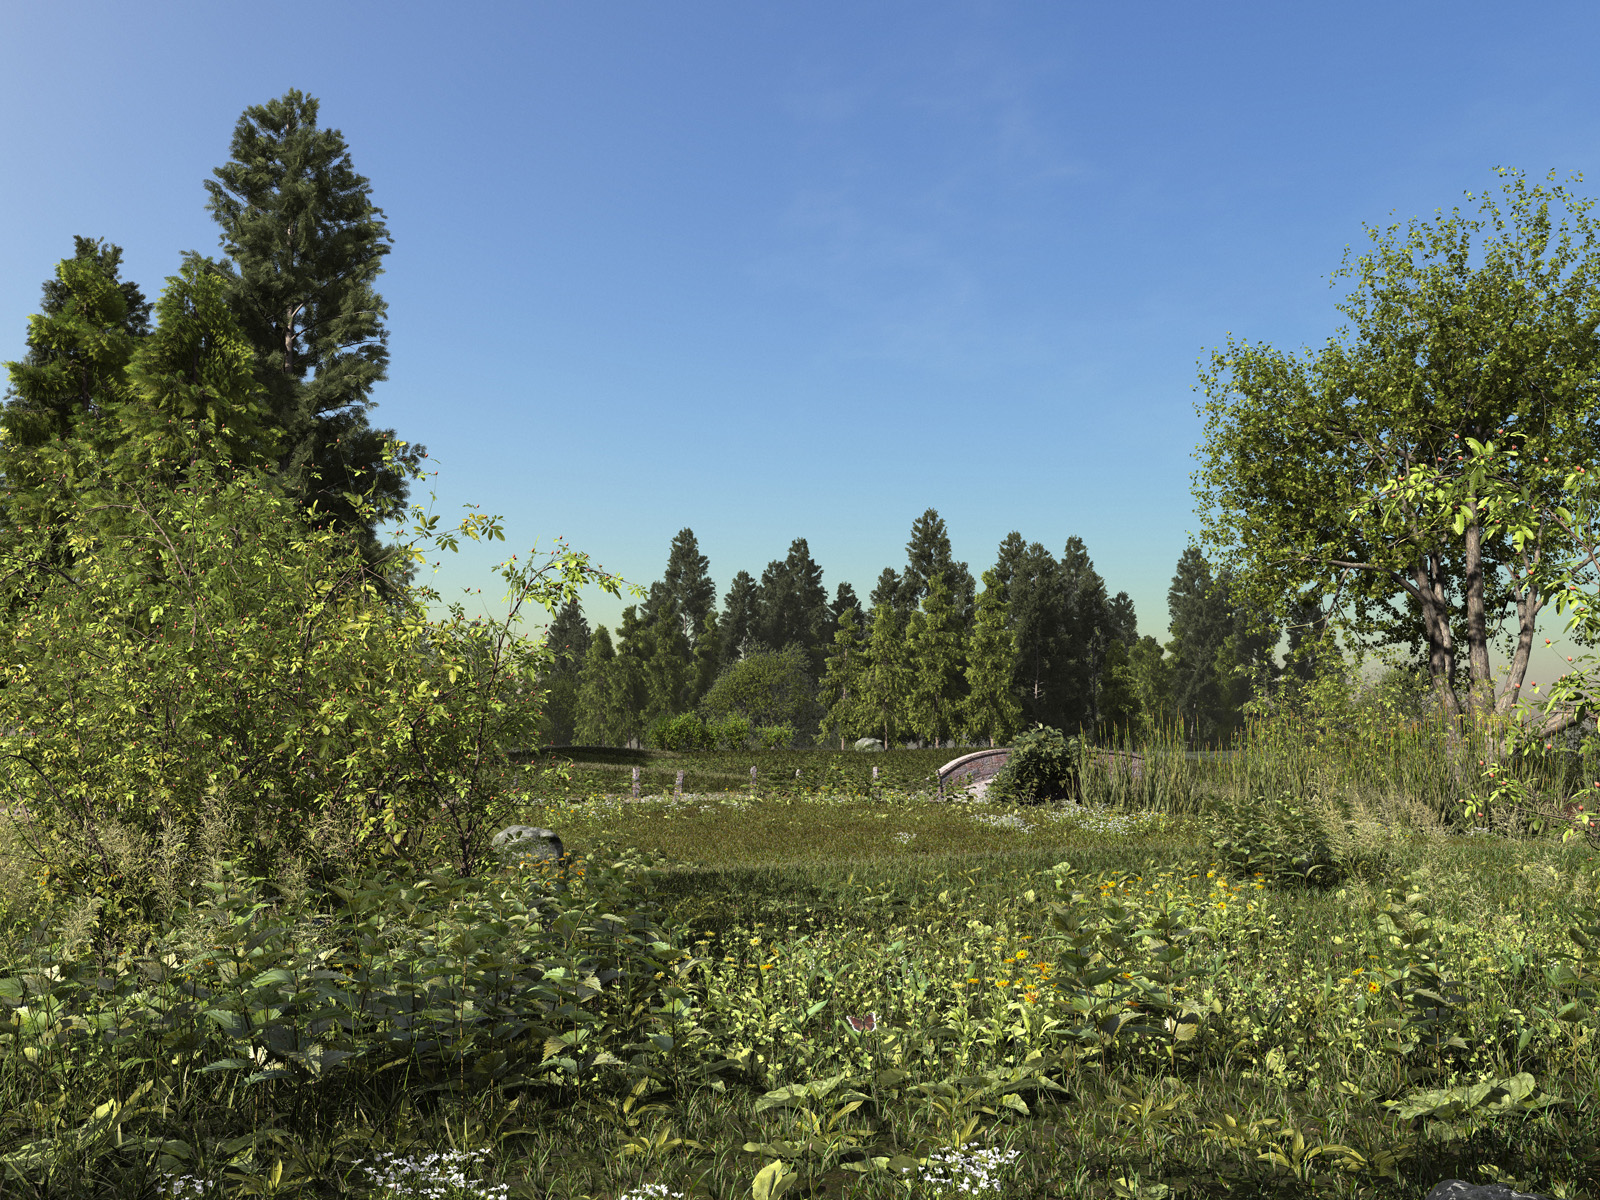
\includegraphics[width=.7\textwidth]{images/greenXfrog_JanWalterSchliep.jpg}
	\caption{\glqq Green\grqq{} von Jan Walter Schliep, modelliert mithilfe der prozeduralen 3D-Modellierungssoftware für Vegetation \glqq Xfrog\grqq. \cite{GreenOne:16}}
	\label{fig:greenXfrog_JanWalterSchliep}
\end{figure}

Die Generierung von Pflanzenmodellen stellt einen großen Bereich der prozeduralen Modellgenerierung dar, da es nur in Ausnahmefällen möglich ist Szenen von Außenbereichen zu erzeugen ohne Vegetation darzustellen. Die Komplexität dieser Thematik wird bereits bei der Betrachtung einzelner Pflanzen deutlich und erstreckt sich von der Modellierung eines einzelnen Blattes über die Positionierung der Blätter auf einer Pflanze bis hin zur Verteilung dieser Vegetation in einer Landschaft. \cite[S.3]{Deussen:05} Eine simple Wiederverwendung von Modellen wird schnell bemerkt und führt zu einem unnatürlichen Eindruck bei Beobachtern -- die manuelle Gestaltung von 3D-Modellen ist somit selten praktikabel. \cite[S.73]{PCGiG:16}

Bäume stellen auffällige Landschaftsmerkmale dar und sind somit ein wichtiger Bestandteil einer realistischen Umgebungsgestaltung. Im Rahmen dieser Arbeit werden daher zwei unterschiedliche Verfahren für die prozedurale Generierung der Aststrukturen von Bäumen sowie die jeweiligen Implementierungen in einer -- insbesondere für die Verwendung in digitalen Spielen geeigneten -- Echtzeitanwendung vorgestellt. 

\section{Bisherige Arbeiten}

Die Entwicklung von Programmen für die 3D-Modellgenerierung von Baumstrukturen begann mit den Arbeiten von Honda und Fisher sowie den Erweiterungen dieser durch Aono und Kunii. Sie verwendeten einige simple Regeln, die mithilfe von Parametern angepasst werden konnten, um realistisch wirkende Baumstrukturen zu erschaffen. \cite[S.46f]{Deussen:05} \cite[S.1]{SpaceColonizationAlgorithm:07} 

Die bereits zuvor von Aristid Lindenmayer entwickelte Erweiterung von kontextfreien Grammatiken -- Lindenmayer-Systeme -- für die Beschreibung zellulärer Vorgänge und das Verzweigungsverhalten von Pflanzen wurden später von Prusinkiewicz und Lindenmayer zusätzlich erweitert, um die Generierung ähnlicher Baumstrukturen mithilfe dieser Systeme zu ermöglichen. \cite[S.43, 48]{Deussen:05} 

Die von P. Oppenheimer und J. Bloomenthal entwickelten Verfahren basieren auf der rekursiven Generierung von Baumstrukturen. Oppenheimers Vorgehen war inspiriert durch die fraktale Natur von Pflanzen und konzentriert auf die schnelle grafische Repräsentation der Modelle, während Bloomenthal die natürliche Darstellung von Verzweigungen beabsichtigte. \cite[S.49-52]{Deussen:05} 

Weiterhin trugen Reeves und Blau, Weber und Penn, Lintermann und Deussen sowie Prusinkiewicz u.a zur Verbesserung und Erweiterung von rekursiven Prozeduren zur Generierung von realistischen Baumstrukturen bei. \cite[S.1]{SpaceColonizationAlgorithm:07}

Ein Ansatz, der sich vom rekursiven Vorgehen unterscheidet, wurde von Rodkaew u.a. entwickelt und basiert auf der Verteilung von Partikeln in Form einer Baumkrone um daraufhin die Aststruktur iterativ von außen bis zur Wurzel aufzubauen. \cite[S.2]{SpaceColonizationAlgorithm:07} Diesem Ansatz ähnelt das Vorgehen von Runions u.a., welches die Erweiterung eines zweidimensionalen Verfahrens zur Generierung von Blattvenen in den dreidimensionalen Raum darstellt und als Space Colonization Algorithmus (engl. für Raum-Kolonisierungs-Algorithmus) bezeichnet wird. Im Gegensatz zu Rodkaew u.a. wurde jedoch der iterative Aufbau ausgehend von der Wurzel und in Abhängigkeit des verfügbaren Raums zum Wachsen vorgeschlagen. \cite[S.2]{SpaceColonizationAlgorithm:07}


\section{Ansatz}

Im Rahmen dieser Arbeit wurden zwei verschiedene Verfahren implementiert: Die von Aristid Lindenmayer entwickelten Lindenmayer-Systeme sowie der von Runions u.a. entwickelte Space Colonization Algorithmus. 

Lindenmayer-Systeme arbeiten mithilfe einer vorgegebenen Menge von Regeln, um bestimmte Teile einer Zeichenkette durch andere Zeichen zu ersetzen. Diese Regeln verlängern die ursprüngliche Zeichenkette und ermöglichen somit die Generierung von komplexen Zeichenabfolgen. \cite[S.2]{ABOP:04} Um aus den Resultaten Modelldaten zu extrahieren wird die von Prusinkiewicz und Lindenmayer vorgeschlagene Interpretation von Zeichenketten verwendet. \cite[S.6]{ABOP:04}

Der Space Colonization Algorithmus nutzt die biologisch motivierte Simulation von Konkurrenz um Platz zwischen sich entwickelnden Zweigen. Es wird ein bestimmter Wachstumsbereich vorgegeben, in dem Zweige in jeder Iteration des Algorithmus wachsen. \cite[S.5]{SpaceColonizationAlgorithm:07}

Die Wahl dieser Verfahren basiert auf den sich ergänzenden Funktionsweisen: Lindenmayer-Systeme erlauben eine genaue Kontrolle über die generierten Baumstrukturen mithilfe der Definition fester Regeln. Der Space Colonization Algorithmus hingegen ermöglicht, durch die Wahl einiger numerischer Parameter, die Generierung komplexer, auf räumliche Einschränkungen reagierender Baummodelle. \cite[S.5]{SpaceColonizationAlgorithm:07}

Die Verfahren enthalten keine festen Vorgaben in Hinsicht auf die grafische Darstellung der generierten Daten. Um eine Konzentration auf die Implementierung der Ansätze zu ermöglichen, wurde die Unreal Engine 4 als Framework für die visuelle und logische Repräsentation der Baumstrukturen in Echtzeit gewählt. Äste werden vereinfacht als Zylinder dargestellt.

\section{Unreal Engine 4}

Die Unreal Engine 4 ist eine Sammlung von Softwarewerkzeugen für die Entwicklung von digitalen Spielen, Echtzeit-3D-Filmen und Simulationen.\cite{WhatIsUE:17}  Sie bietet Bibliotheken für die Darstellung von 3D-Modellen und erfüllt unter anderem die grundlegenden Aufgaben der Speicherverwaltung, Serialisierung von Objekten, und Verwaltung von Benutzereingaben. \cite{EngineFeatures:17}

Die Engine ist in $C++$ programmiert und der Quellcode ist frei zugänglich. Eine Erstellung von Inhalten ist durch die Programmierung von $C++$ Code oder durch die Verwendung der visuellen Skriptsprache \glqq Blueprint\grqq{} möglich. \cite{WhatIsUE:17}

Die Implementierungen der gewählten Ansätze wurden in $C++$ realisiert. Während die Kapitel \ref{ch:LSysteme} und \ref{ch:SCA}, welche die theoretischen Konzepte der Ansätze behandeln, unabhängig von dem Framework verfasst wurden, verwenden die darauf folgenden Kapitel Unreal Engine 4 spezifische Konzepte. Beispielsweise wurden beide Verfahren auf Grundlage der Actor-Basisklasse implementiert.

Ein Actor (engl. für Akteur) in der Unreal Engine 4 ist ein Objekt, das in einem Level platziert werden kann und eine bestimmte Position, Rotation und Skalierung in der Welt besitzt. Die generierte Baumstruktur wird einem Akteur als Komponente hinzugefügt und kann daraufhin vom Grafiksystem der Engine dargestellt werden. Die Generierung der Modelldaten findet in dem lokalen Koordinatensystem des Akteurs statt -- wird die Position, Rotation oder Skalierung des Akteurs verändert, überträgt sich diese Transformation ebenfalls auf die generierten Modelldaten. Dies ermöglicht eine einfache Positionierung von Baumstrukturen in einem Level, ohne neue Modelldaten generieren zu müssen. \cite{UnrealTerminology:17}

Das Akteur-Framework lässt Transformationen sowie die Eingabe von Parametern über den visuellen Leveleditor der Engine zu und erlaubt somit eine schnelle Änderung von Parameterwerten und Anpassung der Positionen von generierten Baumstrukturen. \cite{UnrealTerminology:17}

\begin{figure} [ht]
	\centering
	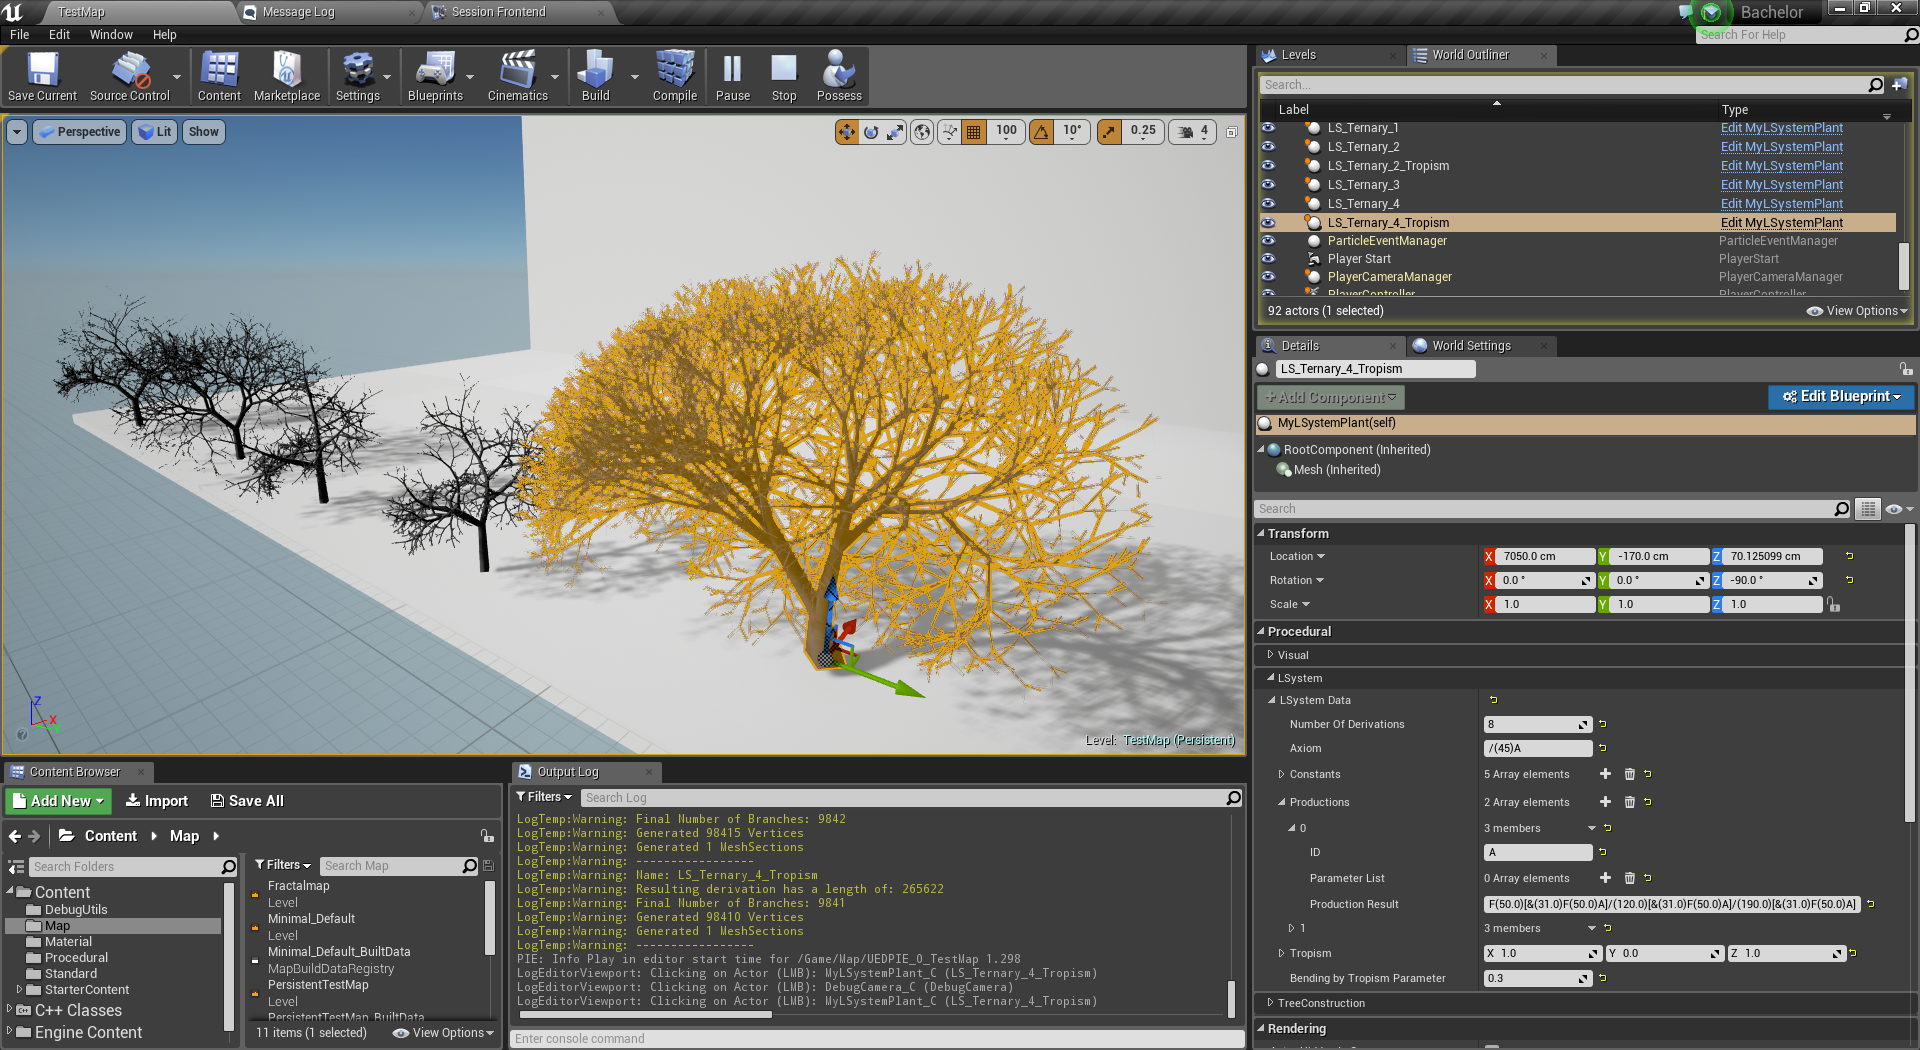
\includegraphics[width=\textwidth]{images/ScreenshotUE4Editor.png}
	\caption{Screenshot des visuellen Leveleditors der Unreal Engine 4. Der aktuell ausgewählte Akteur und seine Komponenten sind gelb hervorgehoben. Die in der Bildmitte dargestellten Pfeile sowie die Eingabefelder im unteren rechten Bildbereich erlauben die Transformation des Akteurs. Ebenfalls im unteren rechten Bildbereich aufgelistet sind weitere Felder um die schnelle Änderung von Parameterwerten zu erlauben, die im $C++$ Quellcode entsprechend definiert sind. }
	\label{fig:ScreenshotUE4Editor}
\end{figure}


Die in den folgenden Kapiteln verwendete Längeneinheit entspricht der in Unreal Engine 4 verwendeten Einheit \grqq$cm$\grqq, das Winkelmaß entspricht der Einheit \glqq Grad\grqq. Alle Abbildungen von Baumstrukturen wurden mithilfe von Screenshots des, im Rahmen dieser Arbeit entwickelten, Projektes erstellt.
\chapter{Lindenmayer-Systeme} \label{ch:LSysteme}

In diesem Kapitel werden Regeln für die Definition von Lindenmayer-Systemen -- kurz: L-Systemen -- festgelegt und die verwendete Methode zur Visualisierung der Ergebnisse von L-Systemen besprochen. Es findet eine Beschränkung des Themas auf die in dieser Arbeit umgesetzten Konzepte statt.

\section{Kontextfreie Grammatik}

Bei L-Systemen handelt es sich um auf Zeichenketten basierende Ersetzungssysteme. Es werden komplexe Objekte beschrieben, indem Teile der Zeichenkette durch andere Zeichen oder Zeichenketten ersetzt werden. Die Beschreibung dieser Ersetzungen findet mittels festgelegter Produktionsregeln statt. \cite[S.2]{ABOP:04} 

Eine formale Definition eines auf Zeichenketten arbeitenden Ersetzungssystems wird durch kontextfreie Grammatiken gegeben:

\newtheorem{defKontextfreieGrammatik}{Kontextfreie Grammatik:}[chapter]
\begin{defKontextfreieGrammatik}
	Eine kontextfreie Grammatik G ist ein Tupel G = $(V, N, P, \omega)$ bestehend aus:
	
	\begin{description}[labelindent]
		\item[\boldmath$V$] Einer nichtleeren, endlichen Menge von Buchstaben (Alphabet).\\
		
		\item[\boldmath$N$] Einer endlichen Menge von Variablen.\\
		
		\item[\boldmath$P$] Einer endlichen Menge von Produktionsregeln in der Form $P: A \rightarrow \alpha$ mit $A \in N$ und $\alpha \in (V \cup N )^*$.\\
		
		\item[\boldmath$\omega \in N$] Dem Axiom, Startsymbol der Grammatik.\\
		
	\end{description}
	\cite[S.343]{ThI:14}
\end{defKontextfreieGrammatik}

Die Menge $V^*$ ist die Menge aller Wörter über $V$, d.h. die Menge aller Wörter, die aus dem Alphabet $V$ gebildet werden können. \cite[S.70]{ThI:14} 

Eine Grammatik wird als kontextfrei bezeichnet, wenn beispielsweise die Produktionsregel $A \rightarrow \alpha$ angewendet werden kann, ohne die $A$ umgebenden Buchstaben -- seinen Kontext -- beachten zu müssen. \cite[S.343]{ThI:14} 

Eine Grammatik wird als deterministisch bezeichnet, wenn es genau eine Produktionsregel $r \in P$ für jede Variable $A \in N$ gibt, sodass $r: A \rightarrow \alpha$, $\alpha \in (V \cup N )^*$. Das bedeutet, dass die Ersetzung einer Variable eindeutig durch eine einzige Regel beschrieben wird. \cite[S.75]{PCGiG:16}

Die Anwendung der Produktionsregeln findet meist sequentiell statt -- die Zeichenkette wird von links nach rechts durchlaufen und Ersetzungen werden direkt auf die untersuchte Zeichenkette angewendet. \cite[S.75]{PCGiG:16}

\section{D0L-Systeme}

Diese Arbeit beschränkt sich auf die Behandlung deterministischer, kontextfreier L-Systeme, auch D0L-Systeme genannt. Diese besitzen die Eigenschaften einer deterministischen und kontextfreien Grammatik, Produktionsregeln werden jedoch parallel und gleichzeitig auf alle Buchstaben des untersuchten Wortes angewendet. Dieses Vorgehen soll die Zellteilung in mehrzelligen Organismen simulieren und ist somit an biologische Vorgänge angelehnt. \cite[S. 3]{ABOP:04} 

Ein D0L-System kann wie folgt definiert werden:
\newtheorem{defD0LSystem}{D0L-System:}[chapter]
\begin{defD0LSystem}
	Ein D0L-System ist ein Tupel G = $(V, P, \omega)$, bestehend aus:
	
	\begin{description}[labelindent]
		\item[\boldmath$V$] Einem nichtleeren, endlichen Alphabet.\\
		
		\item[\boldmath$P$] Einer endlichen Menge von Produktionsregeln in der Form $P: a \rightarrow b$ mit $a \in V$ und $b \in V^*$. $a$ wird als Vorgänger, $b$ als Nachfolger bezeichnet. Ist für einen Buchstaben $x \in V$ keine explizite Produktionsregel angegeben, wird die Identitätsproduktion $P: x \rightarrow x$ angenommen -- der Buchstabe wird durch sich selbst ersetzt.\\
		
		\item[\boldmath$\omega \in V^+$]  Dem Axiom, Startsymbol der Grammatik.		
	\end{description}
\cite[S.4]{ABOP:04} 
\end{defD0LSystem}
Die Menge $V^+$ ist die Menge aller nichtleeren Wörter über $V$. \cite[S.70]{ThI:14}

Die Ableitung eines Wortes entspricht der Ersetzung aller Buchstaben anhand der Produktionsregeln. Ein Wort kann mehrmals abgeleitet werden. 

\newtheorem{defAbleitung}{Ableitung:}[chapter]
\begin{defAbleitung}
	Gegeben sei ein Wort $w = a_1 ... a_m$ mit $w \in V^*$ und $a_i \in V^*$. Das Wort $v = b_1 ... b_m$ mit $v \in V^*$ und $b_i \in V^*$ ist die Ableitung von $w$ wenn für alle $i=1...m$ eine Produktionsregel $a_i \rightarrow b_i$ existiert. Die Ableitung wird als $w \Rightarrow v$ notiert. \\
	Das Wort $w_n$ ist die n-te Ableitung des Wortes $w_0$ wenn eine Folge von Wörtern $w_0, w_1, ..., w_n$ mit Ableitungen $w_0 \Rightarrow w_1 \Rightarrow ... \Rightarrow w_n$ existiert. \cite[S.4]{ABOP:04} 
\end{defAbleitung}


Beispiel: Das Wachstum der Blaualgen-Gattung \glqq Anabaena\grqq{} kann durch ein L-System simuliert werden. Die Buchstaben $a$ und $b$ beschreiben die Größe und Teilungsbereitschaft einer Algenzelle, während die Indizes $l$ und $r$ die Polarität einer Zelle darstellen. Es gelten folgende Produktionsregeln:
\begin{equation}
\begin{array}{cccc}
 p_1 & : a_r &\rightarrow& a_lb_r \\
p_2 &  : a_l &\rightarrow& b_la_r \\ 
p_3 &  : b_r &\rightarrow& a_r \\
p_4 &  : b_l &\rightarrow& a_l 
\end{array}
\label{eq:ProdAnabaena}
\end{equation} 

Die Entwicklung einer Anfangszelle $a_r$ (Axiom $\omega : a_r$) läuft daraufhin wie in Abbildung \ref{fig:AnabaenaAbleitung} dargestellt ab. \cite[S.4]{ABOP:04}
\begin{figure} [hbtp]
	\centering
	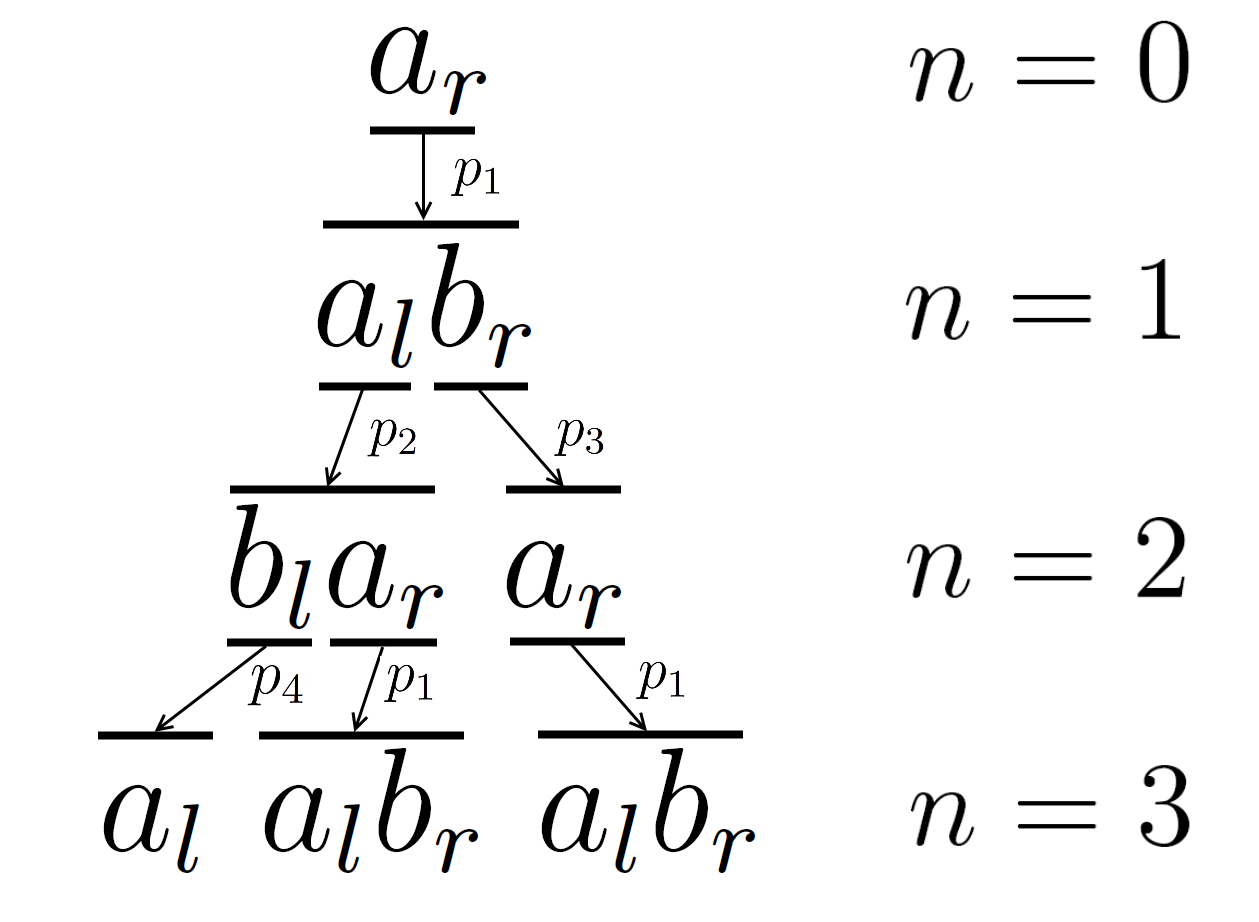
\includegraphics[height=0.25\textheight]{images/AnabaenaAbleitung.png}
	\caption{Die n-fache Ableitung der Anfangszelle $a_r$ anhand der Produktionsregeln $p_1 ... p_4$ aus Gleichung \ref{eq:ProdAnabaena}. Eigene Abbildung auf Grundlage von \cite[S.4]{ABOP:04}.}
	\label{fig:AnabaenaAbleitung}
\end{figure}

\subsection{Parametrische L-Systeme}

Parametrische L-Systeme stellen eine Erweiterung der D0L-Systeme dar. Die Buchstaben eines verwendeten Alphabets $V$ werden um zugeordnete Parameter aus der Menge der reellen Zahlen ergänzt. Ein solches parametrisches Wort $V \times \mathbb{R}^*$ besteht aus einem Zeichen $A \in V$ und Parametern $a_1,...,a_n \in \mathbb{R}$ und wird als $A(a_1,...,a_n)$ dargestellt. Ein parametrisches Wort ohne Parameter mit dem Zeichen $A \in V$  wird schlicht als $A$ dargestellt. \cite[S.41]{ABOP:04}

Die obige Definition von parametrischen Worten geschieht mithilfe von numerischen Konstanten, während bei der Angabe eines L-Systems formale Parameter verwendet werden. Im informatischen Kontext entspricht der Begriff eines formalen Parameters einem Funktionsparameter oder einer Funktionsvariablen. \cite[S.16f]{FormalParamDef:05} 

Ist $\Sigma$ eine Menge von formalen Parametern, dann ist $E(\Sigma)$ ein arithmetischer Ausdruck, in dem Parameter, Konstanten und arithmetische Operatoren auf eine zulässige Weise kombiniert werden. \cite[S.41]{ABOP:04}

\newtheorem{defParametrischeLSysteme}{Parametrisches L-System:}[section]
\begin{defParametrischeLSysteme}
	Ein Parametrisches L-System ist ein Tupel G = $(V, \Sigma, P, \omega)$, bestehend aus:
	\begin{description}[labelindent]
		\item[\boldmath$V$] Einem nichtleeren, endlichen Alphabet.\\
		
		\item[\boldmath$\Sigma$] Einer Menge von formalen Parametern.\\
		
		\item[\boldmath$P$] Einer endlichen Menge von Produktionsregeln $P : (V\times \Sigma^*) \rightarrow (V\times E(\Sigma)*)^*$\\
		
		\item[\boldmath$\omega \in M^+$] mit $M =(V \times \mathbb{R}^*)$ -- einem Axiom in Form eines nichtleeren, parametrischen Wortes.
	\end{description}
\cite[S.41]{ABOP:04}
\end{defParametrischeLSysteme}

Eine Produktionsregel kann auf ein parametrisches Wort angewendet werden wenn das Zeichen, welches dem Wort vorausgeht, und die Anzahl der Parameter mit dem Zeichen und der Parameteranzahl im Vorgänger der Produktionsregel übereinstimmen. \cite[S.42]{ABOP:04}

Beispiel: Gegeben sei folgendes, parametrisches L-System:

\begin{equation}
\begin{array}{llll}
\omega & : A(1,1) \\
p_1 & : A(x,y) &\rightarrow& A(x+1, y*2)\text{ }B(y) \\
p_2 &  : B(x) &\rightarrow& B(x+1)\text{ }C 
\end{array}
\label{eq:ProdParamLSystem}
\end{equation} 

Das Alphabet $V$ und die Menge der formalen Parameter $\Sigma$ gehen implizit aus der Angabe der Produktionsregeln hervor und werden in zukünftigen L-System-Gleichungen nicht angegeben. Die Entwicklung des L-Systems läuft wie in Abbildung \ref{fig:ParamLSystemBeispiel} gezeigt ab. 

\begin{figure} [hbtp]
	\centering
	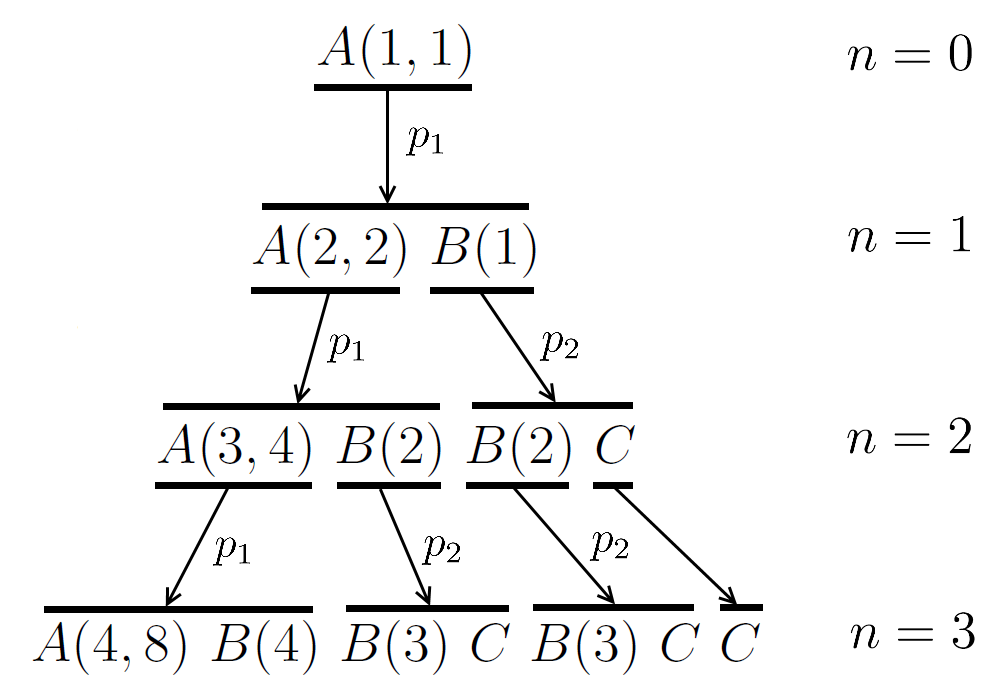
\includegraphics[height=0.3\textheight]{images/ParamLSystemBeispiel.png}
	\caption{Die n-fache Ableitung des Axioms $A(1,1)$ anhand der Produktionsregeln aus Gleichung \ref{eq:ProdParamLSystem}. Die Ersetzung des Zeichens $C$ erfolgt anhand der impliziten Identitätsproduktion. Eigene Abbildung.}
	\label{fig:ParamLSystemBeispiel}
\end{figure}

\section{Grafische Interpretation von L-Systemen}

Um die Ergebnisse von L-Systemen in Form von dreidimensionalen Objekten zu visualisieren, muss eine grafische Interpretation der resultierenden Zeichenketten festgelegt werden. Im Folgenden wird die verwendete Visualisierungsmethode -- die Turtle-Interpretation -- vorgestellt.

\subsection{Turtle-Interpretation}

Die Turtle-Interpretation im zweidimensionalen Raum entspricht der Vorstellung einer Turtle (engl. für Schildkröte) auf einem Blatt Papier. Die Turtle besitzt eine Position $\overrightarrow{p}$ sowie einen Einheitsvektor $\overrightarrow{H}$ in kartesischen Koordinaten. $\overrightarrow{p}$ beschreibt die Position der Turtle auf der Ebene und $\overrightarrow{H}$ entspricht der Blickrichtung (Heading) der Turtle. Der Zustand einer Turtle wird somit vollständig durch die Position und Blickrichtung definiert und wird als Tupel $(\overrightarrow{p},\overrightarrow{H})$ angegeben. \cite[S.2]{Turtle:04} Die Ausgangsposition entspricht dem Ursprung des lokalen Koordinatensystems der Turtle. 

Es können drei Aktionen durchführt werden, welche durch die folgenden Symbole dargestellt werden:

\begin{description}[labelindent]
	\item[\boldmath$F(l)$] Die Turtle bewegt sich um $l>0$ in die Richtung der aktuellen Blickrichtung. Die neue Position ist  $\overrightarrow{p_{neu}}$ mit:
	\begin{equation}
	\begin{array}{ll}
	\overrightarrow{p_{neu}} & = \overrightarrow{p} + l * \overrightarrow{H}
	\end{array}
	\end{equation} 
	Zwischen der alten Position $\overrightarrow{p}$ und der neuen Position $\overrightarrow{p_{neu}}$ wird eine Linie gezeichnet.\\
	
	\item[\boldmath$+(d)$]  Die Turtle dreht sich um den Winkel $d$ nach links. Die neue Blickrichtung ist $\overrightarrow{H'}$ mit:
	\begin{equation}
	\overrightarrow{H'} = 
	\setlength\arraycolsep{10pt}
	\begin{pmatrix}
	cos(d) & -sin(d)\\
	sin(d) & cos(d)
	\end{pmatrix}
	* \overrightarrow{H}
	\end{equation} 
	
	\item[\boldmath$-(d)$]  Die Turtle dreht sich um den Winkel $d$ nach rechts. Die neue Blickrichtung ist $\overrightarrow{H'}$ mit:
	\begin{equation}
	\overrightarrow{H'} = 
	\setlength\arraycolsep{10pt}
	\begin{pmatrix}
	cos(d) & sin(d)\\
	-sin(d) & cos(d)
	\end{pmatrix}
	* \overrightarrow{H}
	\end{equation} 
	
\end{description}
\cite[S.4,46]{Turtle:04} \cite[S.7]{ABOP:04}
Die Symbole \glqq+\grqq{} und \glqq-\grqq{} werden sowohl im Alphabet eines L-Systems als auch bei arithmetischen Operationen in Parameterangaben verwendet, ihre Bedeutung ist abhängig vom Kontext, in dem sie angewendet werden. \cite[S.46]{ABOP:04}

Die grafische Turtle-Interpretation einer Zeichenkette, die durch ein L-System zurückgegeben wird, sind somit die Linien, die auf Grundlage der definierten Symbole gezeichnet werden. 

Beispiel: Mithilfe von L-Systemen und einer Turtle-Interpretation können Fraktale, in diesem Beispiel sogenannte Koch-Kurven, visualisiert werden. Diese Kurven bestehen aus einem Initiator -- einer einfachen, zweidimensionalen Form -- und einem Generator, der einem offenen Polygonzug entspricht. In jedem Ableitungsschritt, angefangen bei dem Initiator, wird jede gerade Linie durch den Generator ersetzt. \cite[S.39]{Mandelbrot:16} 

\begin{figure} [hbtp]
	\centering
	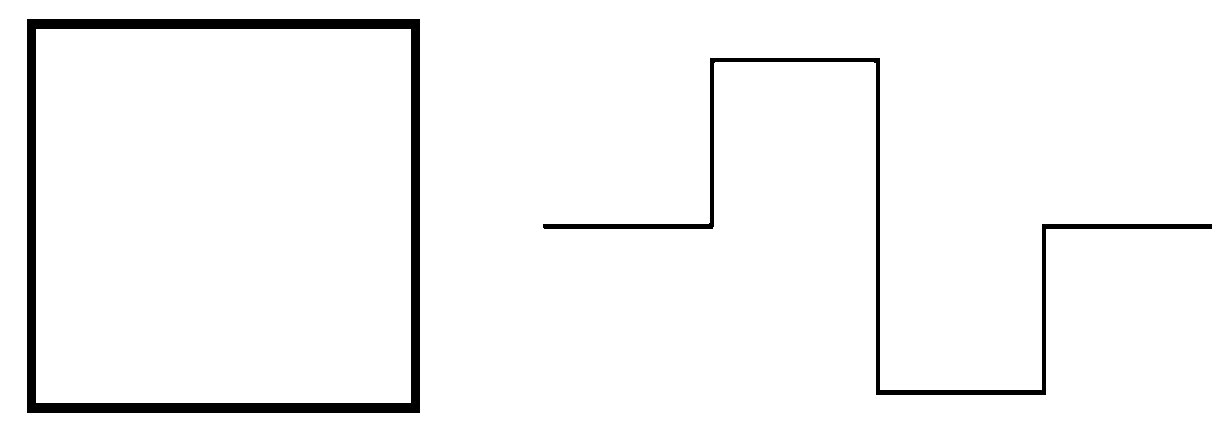
\includegraphics[width=0.6\textwidth]{images/InitiatorGenerator.png}
	\caption{Links: Initiator der Koch-Kurve in Form eines einfachen Quadrats. Rechts: Generator der Koch-Kurve in Form eines offenen Polygonzugs. Eigene Abbildungen.}
	\label{fig:InitiatorGenerator}
\end{figure}

Dieses Verhalten kann nun auf ein L-System abgebildet werden: Der Initiator entspricht dem Axiom und der Generator einer Produktionsregel des L-Systems. Der in Abbildung \ref{fig:InitiatorGenerator} dargestellte Initiator und Generator entsprechen der Turtle-Interpretation des folgenden L-Systems:

\begin{equation}
\begin{array}{llll}
\omega & : F-F-F-F \\
p_1 & : F \rightarrow F+F-F-FF+F+F-F
\end{array}
\label{eq:ProdKochKurve}
\end{equation} 

Für eine bessere Übersicht wurde die Angabe der Parameter weggelassen. Die Turtle interpretiert $F$ als $F(l)$, $-$ als $-(d)$ und $+$ als $+(d)$ mit festgelegter Strichlänge $l$ und Drehwinkel $d$. \label{desc:TurtleWithoutParams} Die Entwicklung des L-Systems läuft, als Turtle-Interpretation visualisiert, wie in Abbildung \ref{fig:KochkurveAbleitung} dargestellt ab.

\begin{figure} [hbtp]
	\centering
	\begin{subfigure}[t]{.4\textwidth}
		
\includegraphics[width=\linewidth]{images/KochkurveN0L400.png}
		\caption{$n=0$, $l=400$, $d=90\degree$}
		\label{fig:KochkurveN0L400}
	\end{subfigure}
	\hspace{.1\textwidth}
	\begin{subfigure}[t]{.4\textwidth}
		\centering
		
\includegraphics[width=\linewidth]{images/KochkurveN1L100.png}
		\caption{$n=1$, $l=100$, $d=90\degree$}
		\label{fig:KochkurveN1L100}
	\end{subfigure}
	\medskip
	\begin{subfigure}[t]{.4\textwidth}
		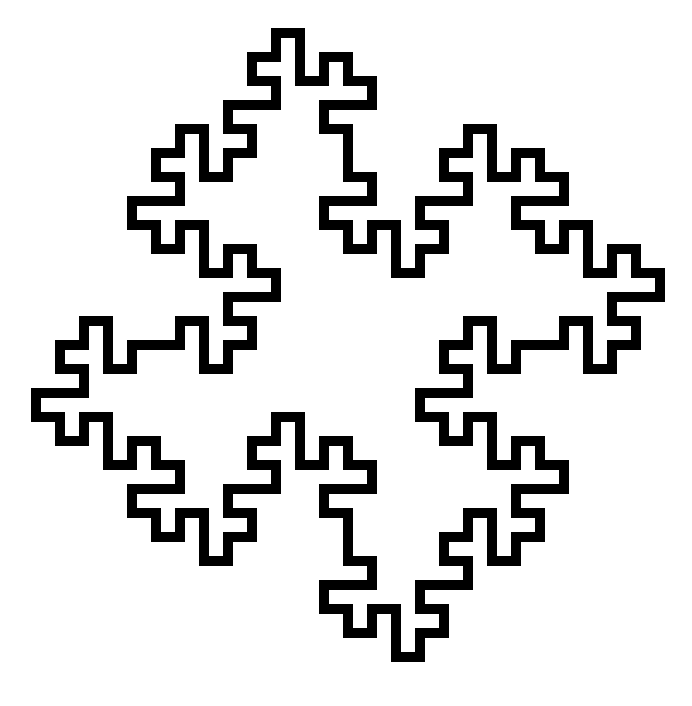
\includegraphics[width=\linewidth]{images/KochkurveN2L25.png}
		\caption{$n=2$, $l=25$, $d=90\degree$}
		\label{fig:KochkurveN2L25}
	\end{subfigure}
	\hspace{.1\textwidth}
	\begin{subfigure}[t]{.4\textwidth}
		\centering
		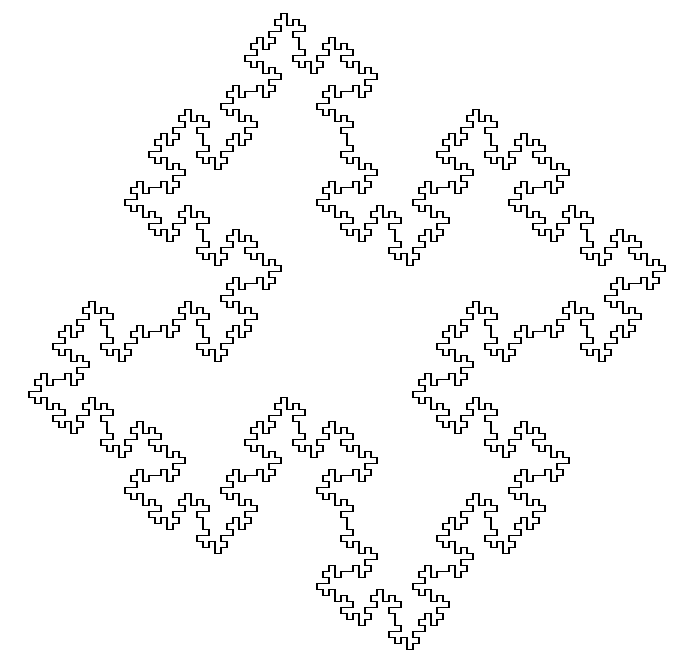
\includegraphics[width=\linewidth]{images/KochkurveN3L6_25.png}
		\caption{$n=3$, $l=6.25$, $d=90\degree$}
		\label{fig:KochkurveN3L6_25}
	\end{subfigure}
	\caption{Die n-fache Ableitung des Axioms $\omega$ anhand der Produktionsregel $p_1$ aus Gleichung \ref{eq:ProdKochKurve}, visualisiert mithilfe der implementierten Turtle-Interpretation. Eigene Abbildungen.}
	\label{fig:KochkurveAbleitung}
\end{figure}

\subsection{Verzweigte L-Systeme} \label{subsec:BranchingLSystems}

Die bisherigen Definitionen von L-Systemen und die korrespondierende Turtle-Interpretation erlaubt lediglich die Bildung von Grafiken mit einem einzelnen, zusammenhängenden Polygonzug. Um L-Systeme zu bilden, deren Visualisierungen Baumstrukturen ähneln, muss die bisherige Turtle-Interpretation um die Möglichkeit erweitert werden Verzweigungen zu verarbeiten. \cite[S.24]{ABOP:04} 

Folgende Operationen werden eingeführt:

\begin{description}[labelindent]
	\item[\textbf{[}] Der aktuelle Zustand der Turtle in Form ihrer Position und Ro\-ta\-tion wird auf einem Stack (engl. für Kellerspeicher) abgelegt. \\
	
	\item[\textbf{]}] Der oberste Zustand der Turtle wird vom Stack genommen. Die aktuelle Position und Rotation der Turtle wird auf die im Zustand gespeicherte Position und Rotation gesetzt. Es wird keine Linie zwischen der alten und neuen Position gezeichnet. 
\end{description}

\cite[S.24]{ABOP:04}

Diese Erweiterung erlaubt es mehrere Linien zu zeichnen, die von einem einzigen Punkt ausgehen und ermöglicht somit die Visualisierung von Abzweigungen. Die Operatoren \textbf{[} und \textbf{]} markieren den Anfang und das Ende eines Zweiges. \cite[S.24]{ABOP:04} 

Beispiel: Mithilfe von verzweigten L-System-Beschreibungen lassen sich die in Abbildung \ref{fig:BranchingLSystems} gezeigten Strukturen bilden. Die Turtle-Interpretation folgt der in \ref{desc:TurtleWithoutParams} beschriebenen Interpretation mit fester Strichlänge $l$ und festem Drehwinkel $d$.

\begin{figure} [hbtp]
	\centering
	\begin{subfigure}[t]{.4\textwidth}
		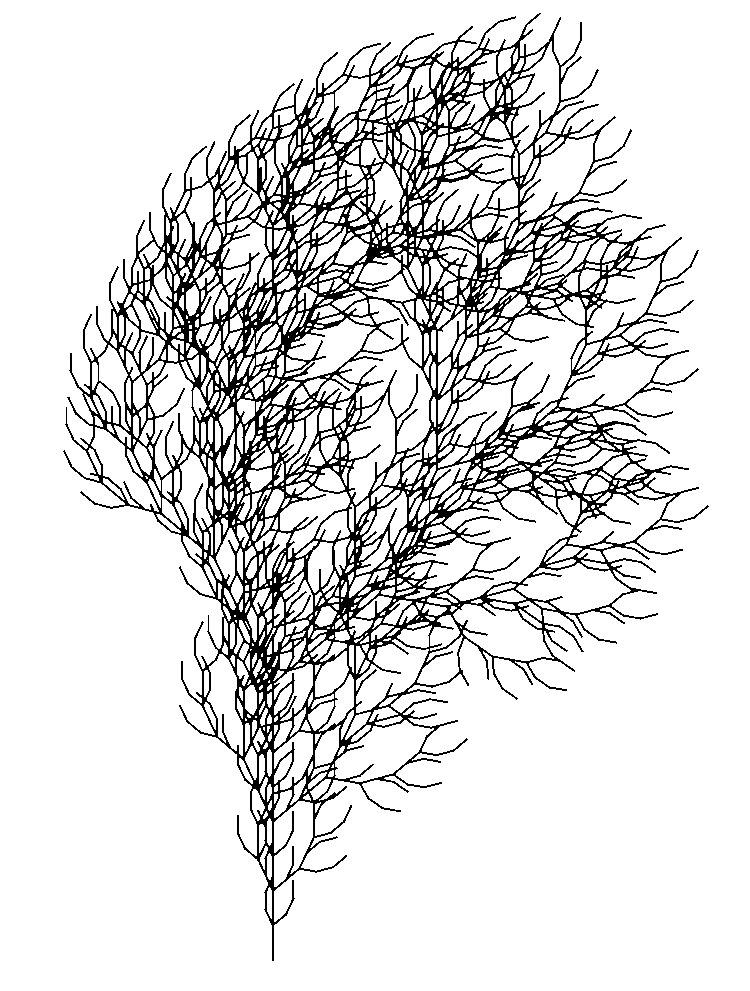
\includegraphics[width=\linewidth]{images/Branching1_N4L18D25.png}
		\caption{$n=4$, $l=18$, $d=25\degree$\\ \\
			$\begin{array}{ll}
				\omega & : F \\
				p_1 & : F \rightarrow FF-[-F+F+F]+[+F-F-F]
			\end{array}
			\label{eq:ProdBranching1}$\\
			\cite[S.25]{ABOP:04}
		}
		\label{fig:Branching1L18D25}
	\end{subfigure}
	\hspace{.15\textwidth}
	\begin{subfigure}[t]{.4\textwidth}
		\centering
		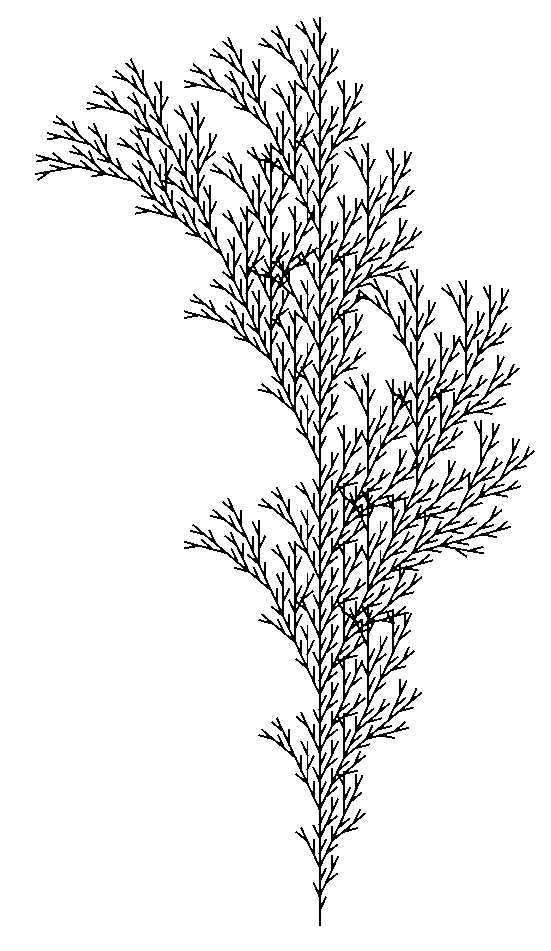
\includegraphics[width=\linewidth]{images/Branching2_N5L15D25.png}
		\caption{$n=5$, $l=15$, $d=25\degree$\\ \\
			$\begin{array}{ll}
				\omega & : F \\
				p_1 & : F \rightarrow F[-F]F[+F][F]
			\end{array}
			\label{eq:ProdBranching2}$\\
			\cite[S.78]{PCGiG:16}
		}
		\label{fig:Branching2L15D25}
	\end{subfigure}

	\caption{Die n-fache Ableitung der Axiome anhand der Produktionsregeln, visualisiert mithilfe der implementierten Turtle-Interpretation. Eigene Abbildung.}
	\label{fig:BranchingLSystems}
\end{figure}

\subsection{Erweiterung der Turtle-Interpretation in den dreidimensionalen Raum}

Die bisherige Definition eines Turtle-Zustands mithilfe einer zweidimensionalen Position und einer Blickrichtung genügt nicht, um Visualisierungen von L-Systemen in Form von dreidimensionalen Baumstrukturen zu ermöglichen. Sowohl die Zustands-Definition als auch die interpretierten Operationen müssen angepasst und erweitert werden.

Der Zustand der Turtle im dreidimensionalen Raum besitzt eine Position $\overrightarrow{p}$ sowie eine $3\times3$ Rotationsmatrix $\boldsymbol{R}$, welche die Orientierung der Turtle im Raum beschreibt. Der Zustand wird als Tupel $(\overrightarrow{p}, \boldsymbol{R})$ angegeben. $\boldsymbol{R}$ entspricht zu Anfang einer Identitätsmatrix. Die Einheitsvektoren $\overrightarrow{H}$, $\overrightarrow{L}$ und $\overrightarrow{U}$  sind orthogonal zueinander und bilden das lokale Koordinatensystem der Turtle. 

\begin{description}[labelindent]
		\item[\boldmath$\overrightarrow{H}$]Die Blickrichtung (Heading-Vektor) der Turtle. Eine Rotation um diesen Vektor um den Winkel $d$ entspricht der Rotationsmatrix $R_{\overrightarrow{H}}(d)$:\\
		\begin{equation}
		R_{\overrightarrow{H}}(d) = 
		\setlength\arraycolsep{10pt}
		\begin{pmatrix}
		1	 	& 0			& 0 \\
		0		& cos(d)	& sin(d) \\
		0 		& -sin(d)	& cos(d)
		\end{pmatrix}	
		\label{eq:rotH}
		\end{equation} 
		
		\item[\boldmath$\overrightarrow{L}$] Der Vektor, der im lokalen Koordinatensystem der Turtle nach links zeigt (Left-Vektor). Eine Rotation um diesen Vektor um den Winkel $d$ entspricht der Rotationsmatrix $R_{\overrightarrow{L}}(d)$:\\
		\begin{equation}
		R_{\overrightarrow{L}}(d) = 
		\setlength\arraycolsep{10pt}
		\begin{pmatrix}
		cos(d) 	& 0		 	& sin(d) \\
		0		& 1			& 0 \\
		-sin(d)	& 0 		&  cos(d)
		\end{pmatrix}	
		\label{eq:rotL}
		\end{equation} 
		
		\item[\boldmath$\overrightarrow{U}$]Der Vektor, der im lokalen Koordinatensystem der Turtle nach oben zeigt (Up-Vektor). Eine Rotation um diesen Vektor um den Winkel $d$ entspricht der Rotationsmatrix $R_{\overrightarrow{U}}(d)$:\\
		\begin{equation}
		R_{\overrightarrow{U}}(d) = 
		\setlength\arraycolsep{10pt}
		\begin{pmatrix}
		cos(d) 	& -sin(d) 	& 0 \\
		sin(d)	& cos(d) 	& 0 \\
		0 		& 0 		& 1
		\end{pmatrix}	
		\label{eq:rotU}
		\end{equation} 
		
	
\end{description}
\cite[S.19]{ABOP:04} \cite[S.69]{Deussen:05} \\

Die erweiterte Turtle-Interpretation verarbeitet folgende Symbole:

\begin{description}[labelindent]
	\item[\boldmath$F(l)$]  Die Turtle bewegt sich um $l>0$ in Blickrichtung $\overrightarrow{H}$. Die neue Position ist $\overrightarrow{p_{neu}}$ mit:
	\begin{equation}
	\begin{array}{ll}
	\overrightarrow{p_{neu}} & = \overrightarrow{p} + l * (\boldsymbol{R} * \overrightarrow{H})
	\end{array}
	\label{eq:Turtle3D_F}
	\end{equation} 
	Zwischen der alten Position $p$ und der neuen Position $p_{neu}$ wird eine Linie gezeichnet. \\
	
	\item[\boldmath$+(d)$]  Die Turtle dreht sich nach links um den Winkel $d$. Die neue Rotationsmatrix entspricht $\boldsymbol{R'}$ mit:\\
	\begin{equation}
	\begin{array}{ll}
	\boldsymbol{R'} & =  \boldsymbol{R} * R_{\overrightarrow{U}}(d)
	\end{array}
	\end{equation} 
	
	\item[\boldmath$-(d)$]  Die Turtle dreht sich nach rechts um den Winkel $d$. Die neue Rotationsmatrix entspricht $\boldsymbol{R'}$ mit:\\
	\begin{equation}
	\begin{array}{ll}
	\boldsymbol{R'} & =  \boldsymbol{R} * R_{\overrightarrow{U}}(-d)
	\end{array}
	\end{equation} 
	
	\item[\boldmath$\&(d)$]  Die Turtle neigt sich nach unten um den Winkel $d$. Die neue Rotationsmatrix entspricht $\boldsymbol{R'}$ mit:\\
	\begin{equation}
	\begin{array}{ll}
	\boldsymbol{R'} & =  \boldsymbol{R} * R_{\overrightarrow{L}}(d)
	\end{array}
	\end{equation}
	
	\item[\boldmath$^\wedge (d)$]  Die Turtle neigt sich nach oben um den Winkel $d$. Die neue Rotationsmatrix entspricht $\boldsymbol{R'}$ mit:\\
	\begin{equation}
	\begin{array}{ll}
	\boldsymbol{R'} & =  \boldsymbol{R} * R_{\overrightarrow{L}}(-d)
	\end{array}
	\end{equation}
	
	\item[\boldmath$\backslash(d)$]  Die Turtle rollt sich nach links um den Winkel $d$. Die neue Rotationsmatrix entspricht $\boldsymbol{R'}$ mit:\\
	\begin{equation}
	\begin{array}{ll}
	\boldsymbol{R'} & =  \boldsymbol{R} * R_{\overrightarrow{H}}(d)
	\end{array}
	\end{equation}
	
	\item[\boldmath$/(d)$]  Die Turtle rollt sich nach rechts um den Winkel $d$. Die neue Rotationsmatrix entspricht $\boldsymbol{R'}$ mit:\\
	\begin{equation}
	\begin{array}{ll}
	\boldsymbol{R'} & =  \boldsymbol{R} * R_{\overrightarrow{H}}(-d)
	\end{array}
	\end{equation}
\end{description}
\cite[S.19]{ABOP:04} \cite[S.69]{Deussen:05}

Mithilfe der Turtle-Interpretation im dreidimensionalen Raum können nun L-Systeme visualisiert werden, die realen Baumstrukturen ähneln. Ein Beispiel dafür ist das L-System aus Gleichung \ref{eq:3DTreeP61B_Prod}, dargestellt in Abbildung \ref{fig:BranchingLSystems3D}.

\begin{equation}
	\begin{array}{llll}
	\omega :&  /(45)\text{ }A \\
	p_1 :&  A &\rightarrow & F(50)\text{ }[\&(a)F(50)A]\text{ }/(d)\text{ }[\&(a)F(50)A]\text{ }/(d)\text{ }[\&(a)F(50)A] \\
	p_2 :& F(l) &\rightarrow & F(l*l_r)
	\end{array}
	\label{eq:3DTreeP61B_Prod}
\end{equation}

	\cite[S.60]{ABOP:04} 
\begin{figure} [hbtp]
	\centering
	\begin{subfigure}[t]{.7\textwidth}
		\centering
		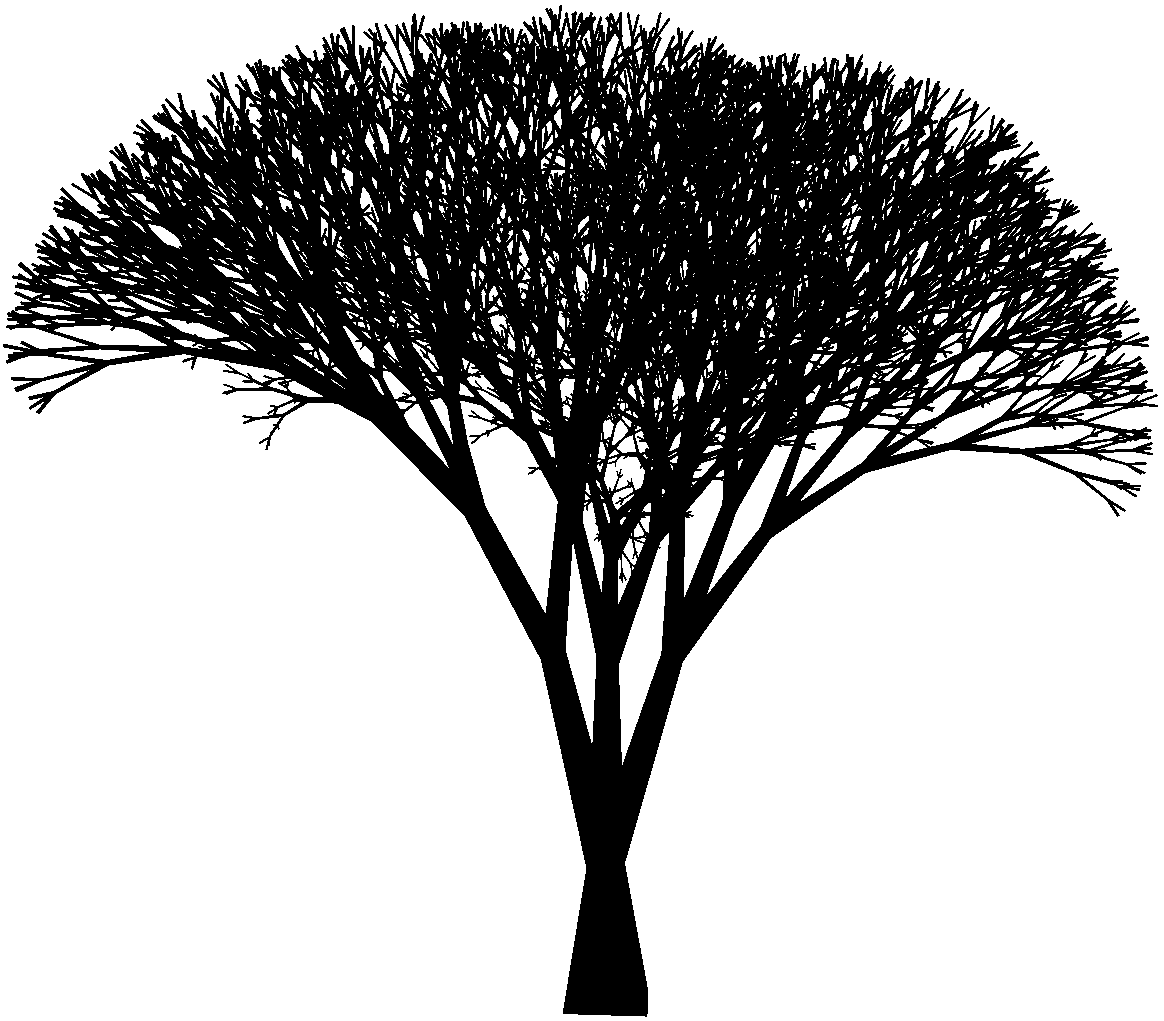
\includegraphics[width=\linewidth]{images/3DTreeP61B_Angle_18_95.png}
		\caption{$n=8$, $d=137.5\degree$, $a=18.95\degree$, $l_r=1.3$}
		\label{subfig:3DTreeP61B_Angle_18_95}
	\end{subfigure}
	\begin{subfigure}[t]{.7\textwidth}
		\centering
		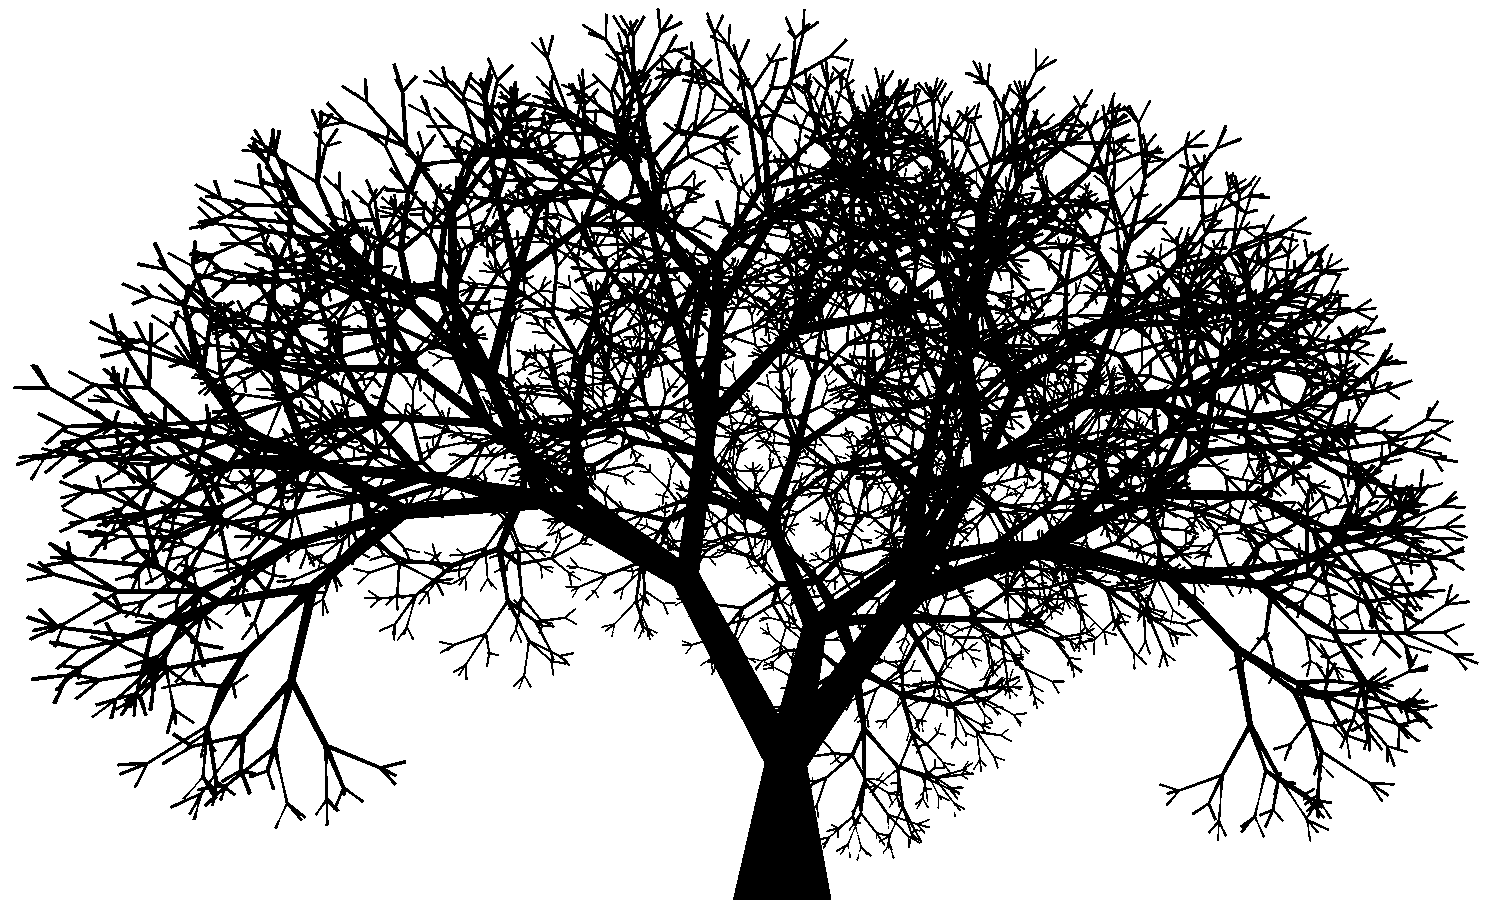
\includegraphics[width=\linewidth]{images/3DTreeP61B_Angle_36.png}
		\caption{$n=8$, $d=137.5\degree$, $a=36.0\degree$, $l_r=1.3$}
		\label{subfig:3DTreeP61B_Angle_36}
	\end{subfigure}
	\caption{Die n-fache Ableitung des Axioms anhand der Produktionsregeln aus Gleichung \ref{eq:3DTreeP61B_Prod}, visualisiert mithilfe der implementierten Turtle-Interpretation. Eigene Abbildungen.}
	\label{fig:BranchingLSystems3D}
\end{figure}

\section{Anpassungen für Baumstrukturen}\label{sec:LS_Baumstrukturen}

Die Darstellung von verzweigten L-Systemen mithilfe von Zeichenketten ermöglicht eine Repräsentation in Textform und erlaubt die einfache Definition von Produktionsregeln. Um jedoch eine effiziente Nachbearbeitung und Visualisierung der Ergebnisse eines L-Systems zu ermöglichen, müssen die Aktionen einer Turtle als graphentheoretischer Baum festgehalten werden. Weiterhin wird der Begriff des Tropismus und dessen Einfluss auf die Modellierung von Baumstrukturen eingeführt.

\subsection{Graphentheoretische Bäume}

Ein Baum, in der Graphentheorie, ist ein kreisfreier Graph $G = \langle V,E\rangle$ für den folgende Begriffe festgelegt werden:

\begin{description}[labelindent]
	\item[\boldmath$V$] Die Menge der Knoten. Jeder Knoten entspricht einem Punkt $\overrightarrow{p_v}$ im dreidimensionalen Raum. \cite[S.358]{ThI:14}\\
	
	\item[\boldmath$E$] Die Menge der Kanten, welche die Vorgänger-Nachfolger-Beziehungen zwischen den Knoten darstellt. Eine Kante $e \in E$ wird als Tupel $e = (v_1, v_2)$ mit $v_1, v_2 \in V$ dargestellt. $v_1$ wird als Vorgänger von $v_2$ und $v_2$ als Nachfolger von $v_1$ bezeichnet. Jeder Knoten besitzt maximal einen Vorgänger und eine endliche Menge von Nachfolgern. \cite[S.358]{ThI:14} \cite[S.29]{AlgoDat:14}\\
	
	\item[\boldmath$Wurzel$] Eine Wurzel ist ein Knoten $v \in V$ ohne einen Vorgänger. Der Baum besitzt genau eine Wurzel. \cite[S.358]{ThI:14}\\
	
	\item[\boldmath$Grad$] Der Grad eines Knotens ist definiert als die Anzahl seiner Nachfolger. \cite[S.29]{AlgoDat:14}\\
	
	\item[\boldmath$Tiefe$] Die Tiefe eines Knotens ist definiert als die Länge der Folge von Vorgängern, die durchlaufen werden muss, bis die Wurzel erreicht wurde. Die Wurzel besitzt die Tiefe $0$. \cite[S.30]{AlgoDat:14}
\end{description}

Ein Baum ist grundsätzlich ein rein topologisches Objekt, mithilfe der Zuordnung von Punkten zu Knoten kann jedoch eine geometrische Vorstellung des Aufbaus bewirkt werden. \cite[S.23]{ABOP:04}

 Um den Aufbau eines Baumes $G = \langle V,E \rangle$ mithilfe der Turtle-Interpretation zu ermöglichen, muss der Turtle-Zustand um einen Knotenpunkt $v \in V$ ergänzt werden. Der Zustand wird als Tupel $(\overrightarrow{p}, v, \boldsymbol{R})$ angegeben. 
 
 Die Turtle-Interpretation beginnt mit der Erstellung der Wurzel am Ursprung des lokalen Bezugssystems. Die Verarbeitung folgender Symbole muss erweitert werden:

\begin{description}[labelindent]
		\item[\boldmath$F(l)$]  Die neue Position $\overrightarrow{p_{neu}}$ der Turtle wird entsprechend Gleichung \ref{eq:Turtle3D_F} berechnet. An diesem Punkt wird ein Knoten $v_{neu}$ und eine Kante $(v,v_{neu})$ erstellt sowie $v$ als Vorgänger von $v_{neu}$ und $v_{neu}$ als Nachfolger von $v$ eingetragen. $v$ entspricht dem aktuellen Zustandsknoten der Turtle. Der neue Turtle-Zustand ist $(\overrightarrow{p_{neu}}, v_{neu}, \boldsymbol{R})$.  \\
	
	\item[\boldmath$\textbf{[}$] Zusätzlich zu der Position und Rotation der Turtle wird auch der aktuelle Knoten auf einem Stack abgelegt.\\
	
	\item[\boldmath$\textbf{]}$] Der oberste Zustand der Turtle wird vom Stack genommen. Zusätzlich zur Position und Rotation wird auch der Zustandsknoten der Turtle auf den gespeicherten Knoten gesetzt.\\
\end{description}

Die Kanten zwischen Knoten wurden durch die Turtle-Interpretation bisher als Linien visualisiert und können als Astsegmente von echten Baumstrukturen verstanden werden. \cite[S.23]{ABOP:04} Die Repräsentation von Turtle-Aktionen als graphentheoretischer Baum ermöglicht die in Abschnitt \ref{sec:Modellgenerierung} beschriebene Generierung und Nachbearbeitung von Modelldaten.

\subsection{Tropismus}

Tropismus ist die Tendenz einer Pflanze in eine bestimmte Richtung zu wachsen, beispielsweise aufgrund einer Lichtquelle oder der Beugung durch Gravitation. \cite[Abschn. 3]{SpaceColonizationAlgorithm:07} Der Einfluss von Tropismus wird als ein dreidimensionaler Vektor $\overrightarrow{T}$ angegeben. Die Bewegung $F(l)$ der Turtle wird wie folgt erweitert:

\begin{description}[labelindent]
	\item[\boldmath$F(l)$]  Die Turtle bewegt sich um $l>0$ in Blickrichtung $\overrightarrow{H}$. Die neue Position ist $\overrightarrow{p_{neu}}$ mit:
	\begin{equation}
	\begin{array}{ll}
	\overrightarrow{p_{neu}} & = \overrightarrow{p} + l * \dfrac{\overrightarrow{H_{rot}} + e * \overrightarrow{T} }{\lVert \overrightarrow{H_{rot}} + e * \overrightarrow{T} \rVert} 
	\end{array}
	\end{equation} 
	
	\begin{equation}
	\begin{array}{ll}
	\text{ und } \overrightarrow{H_{rot}} & = \boldsymbol{R} * \overrightarrow{H}
	\end{array}
	\end{equation} 
	
\end{description}

wobei $e$ der Anfälligkeit des Baums für die Beugung durch Tropismus entspricht, im Folgenden als Biegsamkeitsfaktor bezeichnet. \cite[S.58]{ABOP:04} \cite[Abschn. 3]{SpaceColonizationAlgorithm:07}
\begin{figure} [hbtp]
	\centering
	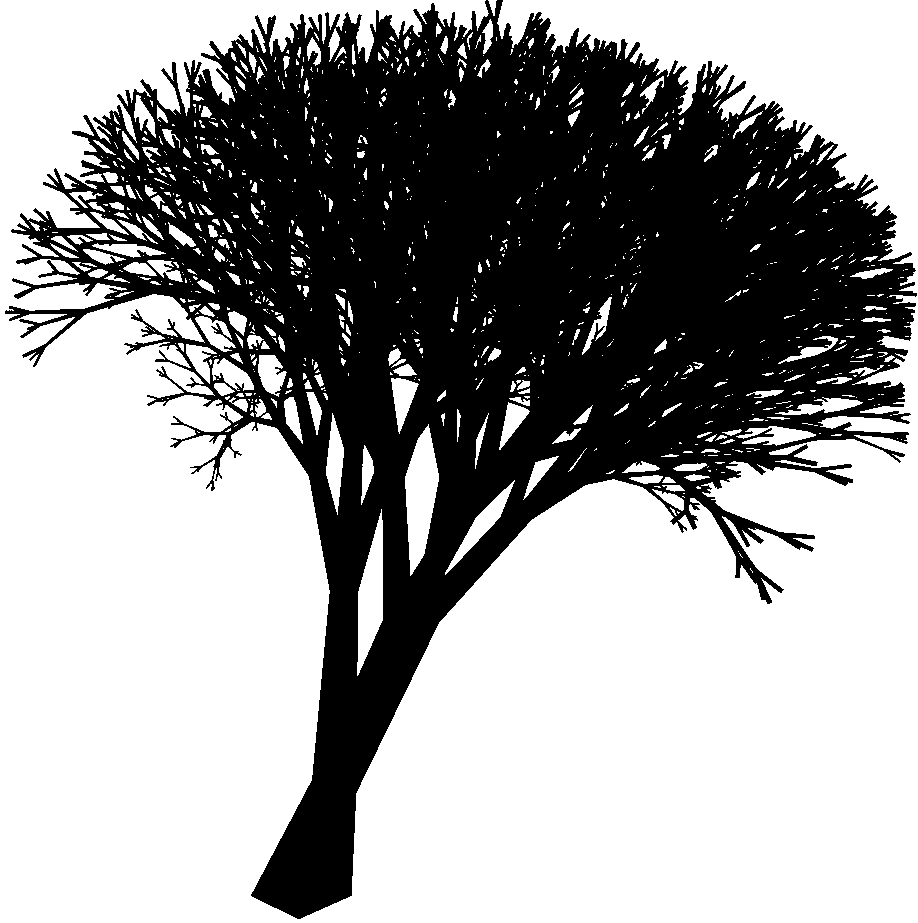
\includegraphics[width=.6\textwidth]{images/3DTreeP61B_Angle_18_95_Tropism.png}
	\caption{.\\
		$n=8$, $d=137.5\degree$, $a=36.0\degree$, $l_r=1.3$, $\protect\overrightarrow{T} =\protect\begin{pmatrix}
		0 \\ 1 \\ -0.5
		\protect\end{pmatrix}$, $e = 0.27$\\
		Die n-fache Ableitung des Axioms anhand der Produktionsregeln aus Gleichung \ref{eq:3DTreeP61B_Prod}, visualisiert mithilfe der erweiterten Turtle-Interpretation. Zeigt den Einfluss von Tropismus auf den in Abbildung \ref{subfig:3DTreeP61B_Angle_18_95} dargestellten Baum.  Eigene Abbildung.}
	\label{fig:3DTreeP61B_Angle_18_95_Tropism}
\end{figure}
\chapter{Space Colonization Algorithmus} \label{ch:SCA}

Es werden die benötigten Eingaben und der Ablauf des Space Colonization Algorithmus behandelt. Die Prozedur zur Generierung von Baumstrukturen wird vorgestellt und die implementierten Erweiterungen des ursprünglichen Algorithmus werden erläutert.

\section{Ursprung}
Der vorgestellte Space Colonization Algorithmus wurde ursprünglich zur Modellierung und Visualisierung von Blattvenen entwickelt und basiert auf der Wirkung des Pflanzenhormons Auxin. Dieser Hormonstoff entsteht im Blatt und wird von bereits existierenden Blattvenen angezogen, der resultierende Hormonstrom führt zur Bildung von neuen Venen im Blatt. Die Simulation dieses Vorgangs führt zu realitätsnahen Venenmustern. \cite[Abschn. 2.5]{LeafVenation:05}

Mithilfe einer Erweiterung in den dreidimensionalen Raum und Nachbearbeitung der Resultate kann eine Vielfalt von Baum- und Strauchstrukturen generiert werden. \cite[Abschn. 1]{SpaceColonizationAlgorithm:07}

\section{Aufbau}

Der Algorithmus verarbeitet eine Menge von Einflusspunkten $S$ und baut darauf basierend einen Baum $G = \langle V,E \rangle$ auf. 

Der Algorithmus benötigt die folgenden Eingaben:

\begin{description}[labelindent]
	\item[\boldmath$d_i$] Der Einflussradius. Einflusspunkte prägen den Aufbau des Baums nur, wenn sich Knotenpunkte innerhalb dieses Radius befinden. \cite[Abschn. 2]{SpaceColonizationAlgorithm:07}\\
	
	\item[\boldmath$d_k$] Der Minimalradius. Befindet sich ein Knotenpunkt innerhalb des Minimalradius um einen Einflusspunkt, wird dieser aus der Menge der Einflusspunkte $S$ entfernt. \cite[Abschn. 2]{SpaceColonizationAlgorithm:07}\\
	
	\item[\boldmath$D$] Die Schrittweite. Jeder neu generierte Knotenpunkt wird in diesem Abstand zu seinem Vorgänger positioniert. \cite[Abschn. 2]{SpaceColonizationAlgorithm:07} \\
	
	\item[\boldmath$\overrightarrow{T}$] Der Tropismusvektor. 

\end{description}

\section{Ablauf}
\label{sec:SCA_Ablauf}
Zu Beginn des Algorithmus werden $N$ Einflusspunkte in einem vorgegebenen Bereich generiert. Dieser Einflussbereich signalisiert die Verfügbarkeit von Raum, in dem die Baumstruktur entstehen kann.  \cite[Abschn. 2]{SpaceColonizationAlgorithm:07}

Daraufhin wird der Baum iterativ aufgebaut und durchläuft in jeder Iteration die folgenden Schritte: 

\begin{description}[labelindent]
	\item[\boldmath$1.$] Für jeden Einflusspunkt in $S$ wird der am nächsten liegende Knotenpunkt $v\in V$ bestimmt. Befindet sich $v$ innerhalb des Einflussradius $d_i$ eines Einflusspunktes, wird der Knotenpunkt einer zugeordneten Menge $S(v)$ hinzugefügt. $S(v)$ beinhaltet somit alle Einflusspunkte, die einen Einfluss auf den Knotenpunkt ausüben. \cite[Abschn. 2]{SpaceColonizationAlgorithm:07} \label{alg:SCA_1}\\
	
	\item[\boldmath$2.$] Befinden sich Elemente in $S(v)$, wird ein neuer Knotenpunkt $v_n$ den Nachfolgern von $v$ hinzugefügt und $v$ als Vorgänger von $v_n$ eingetragen.  Alle Punkte in $S(v)$ beeinflussen $v_n$ in gleichem Maße, die neue Position $\overrightarrow{p_{v_n}}$ des Knotenpunkts berechnet sich somit wie folgt:
	
	\begin{equation}
	\begin{array}{ll}
	\overrightarrow{p_{v_n}} & = \overrightarrow{p_v} + D * \overrightarrow{n_{T}}
	\end{array}
	\end{equation} 
	
	\begin{equation}
	\begin{array}{ll}
	\text{  mit  } \overrightarrow{n_{T}} & = \dfrac{\overrightarrow{n} + \overrightarrow{T} }{\lVert\overrightarrow{n} + \overrightarrow{T}\rVert}  
	\end{array}
	\end{equation} 
	
	\begin{equation}
	\begin{array}{ll}
	\text{ und }  \overrightarrow{n} = \sum\limits_{s \in S(v)}\dfrac{\overrightarrow{p_s} - \overrightarrow{p_v}}{\lVert \overrightarrow{p_s} - \overrightarrow{p_v} \rVert}
	\end{array}
	\end{equation}	
	\cite[Abschn. 2]{SpaceColonizationAlgorithm:07} \label{alg:SCA_2}\\
	
	\item[\boldmath$3.$] Für jeden Einflusspunkt wird überprüft, ob sich ein Knotenpunkt innerhalb des Minimalradius $d_k$ befindet. Existiert ein solcher Knotenpunkt, wird der Einflusspunkt aus der Menge der Einflusspunkte $S$ entfernt. \cite[Abschn. 2]{SpaceColonizationAlgorithm:07} \label{alg:SCA_3}
\end{description}

Diese Schritte werden solange ausgeführt, bis alle Einflusspunkte entfernt wurden, sich kein Knotenpunkt im Einflussradius eines Einflusspunktes befindet oder bis eine vorgegebene Maximalanzahl von Iterationen durchgeführt wurde. Abbildung \ref{fig:SCA_Basic} zeigt eine beispielhafte Anwendung des Algorithmus.

\begin{figure} [hbtp]
	\centering
	\begin{subfigure}[t]{.31\textwidth}
		\centering
		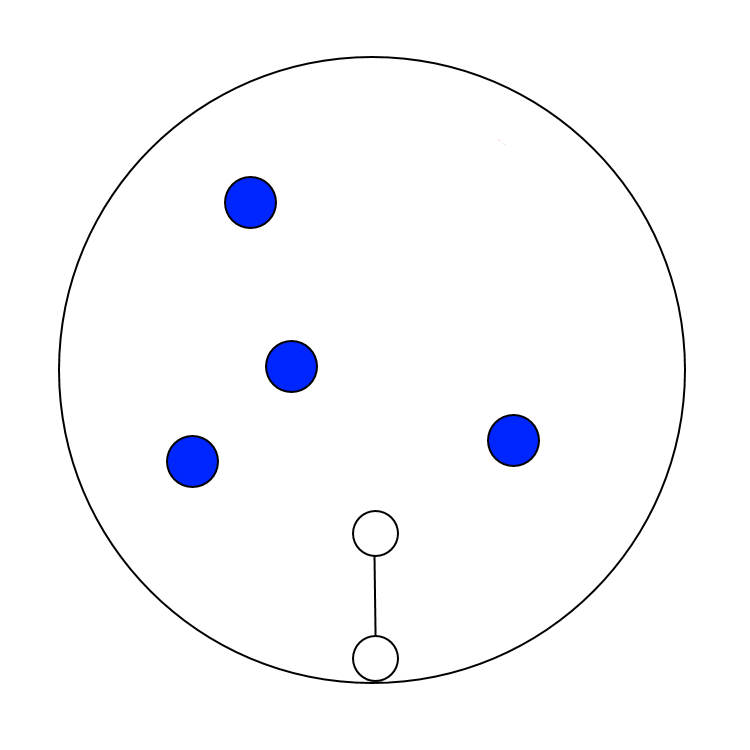
\includegraphics[width=\linewidth]{images/SCA_Basic1.png}
		\caption{ Ausgangssituation. }
		\label{subfig:SCA_Basic1}
	\end{subfigure}
	\hspace{.01\textwidth}
	\begin{subfigure}[t]{.31\textwidth}
		\centering
		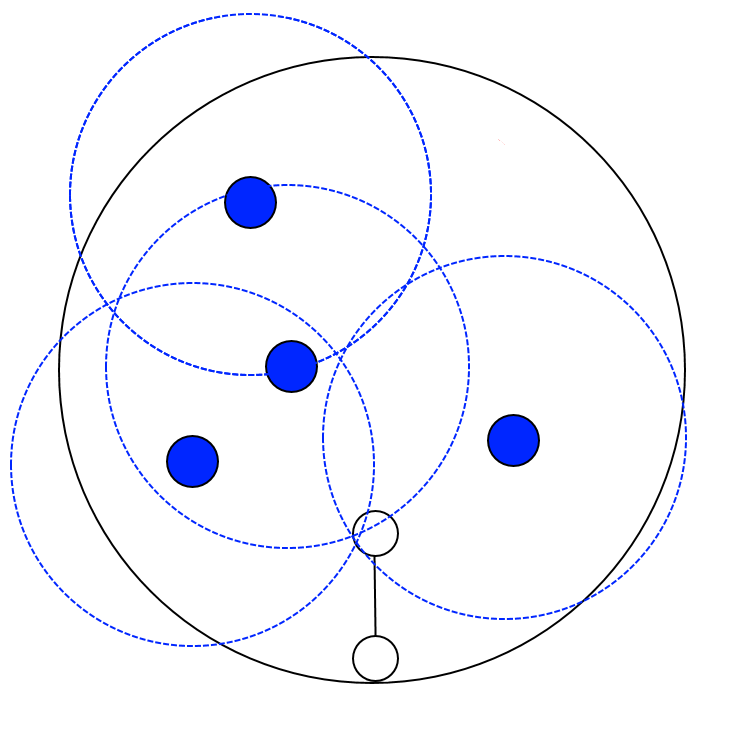
\includegraphics[width=\linewidth]{images/SCA_Basic2.png}
		\caption{Schritt 1: Blaue Kreise entsprechen dem Einflussradius.}
		\label{subfig:SCA_Basic2}
	\end{subfigure}
	\hspace{.01\textwidth}
	\begin{subfigure}[t]{.31\textwidth}
		\centering
		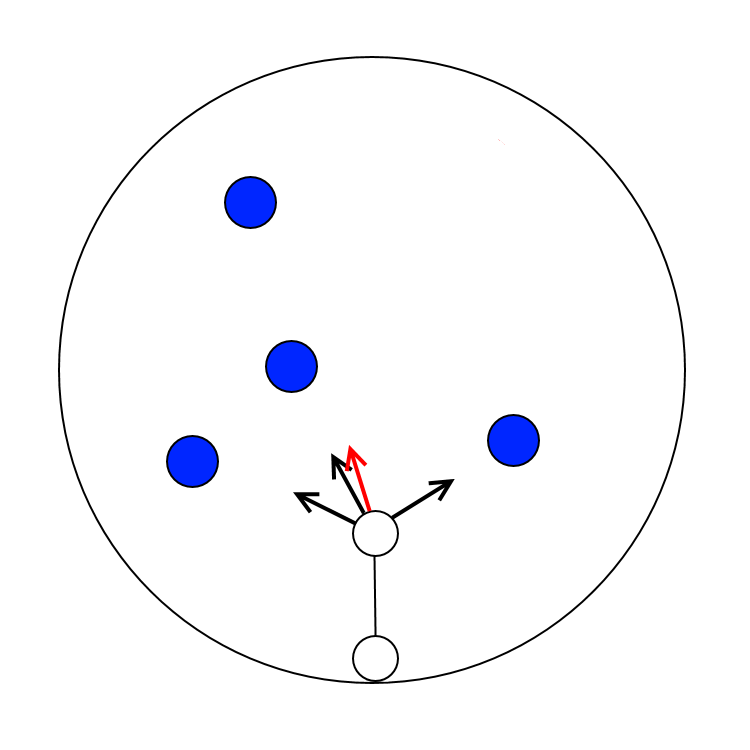
\includegraphics[width=\linewidth]{images/SCA_Basic3.png}
		\caption{Schritt 2: Bestimmung von $\tilde{n}$ (roter Pfeil) ohne Einbeziehung von $\overrightarrow{T}$.}
		\label{subfig:SCA_Basic3}
	\end{subfigure}

	\begin{subfigure}[t]{.31\textwidth}
		\centering
		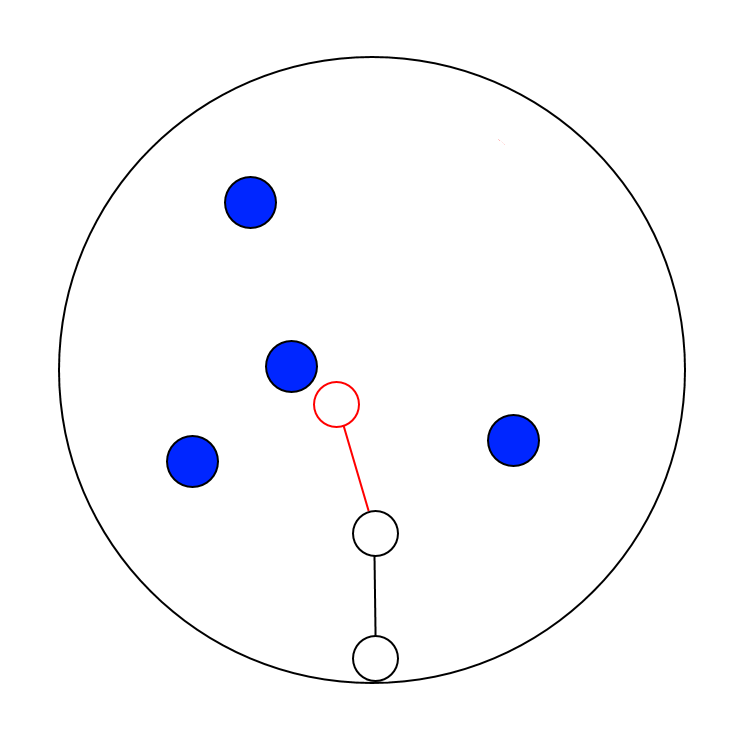
\includegraphics[width=\linewidth]{images/SCA_Basic4.png}
		\caption{Schritt 2: Platzierung des neuen Knotenpunkts.}
		\label{subfig:SCA_Basic4}
	\end{subfigure}
	\hspace{.01\textwidth}
	\begin{subfigure}[t]{.31\textwidth}
		\centering
		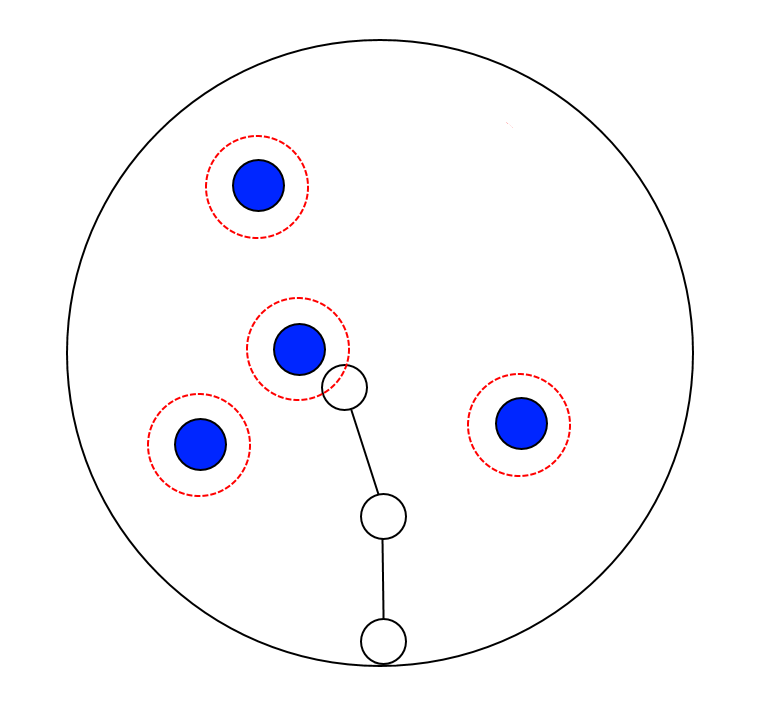
\includegraphics[width=\linewidth]{images/SCA_Basic5.png}
		\caption{Schritt 3: Rote Kreise entsprechen dem Minimalradius.}
		\label{subfig:SCA_Basic5}
	\end{subfigure}
	\hspace{.01\textwidth}
	\begin{subfigure}[t]{.31\textwidth}
		\centering
		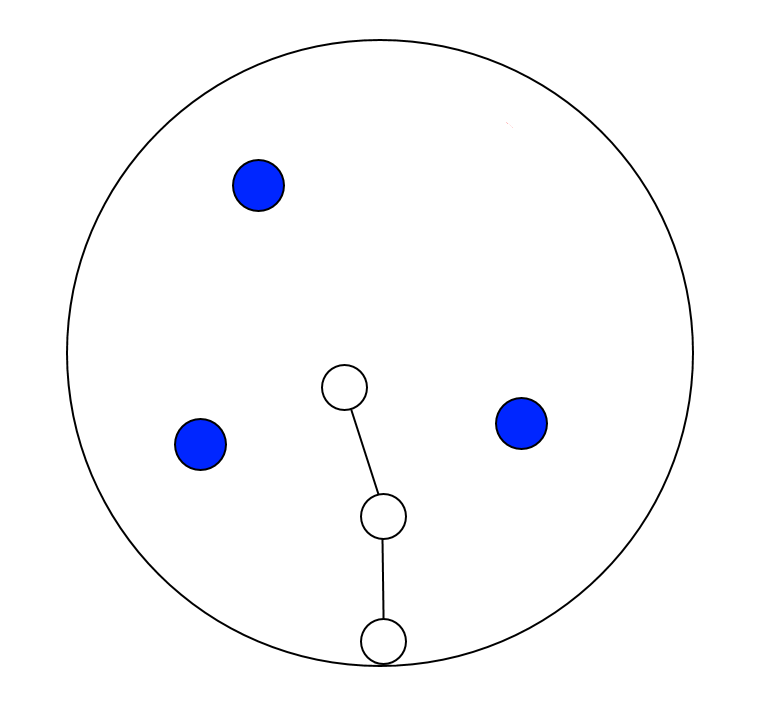
\includegraphics[width=\linewidth]{images/SCA_Basic6.png}
		\caption{Ausgangssituation der nächsten Iteration.}
		\label{subfig:SCA_Basic6}
	\end{subfigure}

	\begin{subfigure}[t]{.31\textwidth}
		\centering
		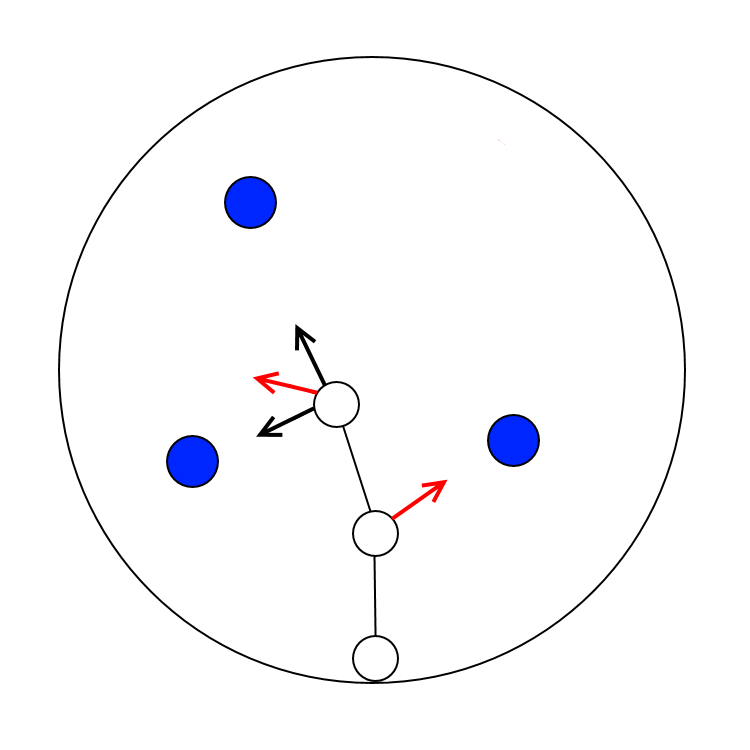
\includegraphics[width=\linewidth]{images/SCA_Basic7.png}
		\caption{Einflusspunkte beeinflussen unterschiedliche Knotenpunkte.}
		\label{subfig:SCA_Basic7}
	\end{subfigure}
	\hspace{.01\textwidth}
	\begin{subfigure}[t]{.31\textwidth}
		\centering
		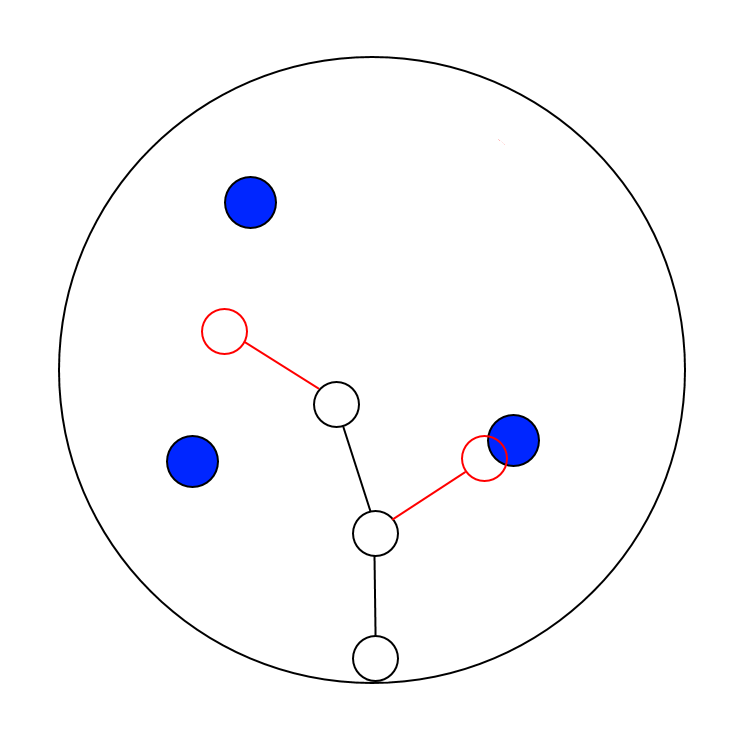
\includegraphics[width=\linewidth]{images/SCA_Basic8.png}
		\caption{Eine Verzweigung entsteht.}
		\label{subfig:SCA_Basic8}
	\end{subfigure}
	\caption{Beispielhafte Anwendung des Space Colonization Algorithmus. Blaue Punkte entsprechen Einflusspunkten, weiße Punkte entsprechen Knotenpunkten. Der unterste Knotenpunkt stellt die Wurzel dar. Eigene Abbildungen auf Grundlage von \cite[Abb. 2]{SpaceColonizationAlgorithm:07}.}\label{fig:SCA_Basic}
	
\end{figure}


\section{Generierung von Baumstrukturen}
\label{sec:GenerierungBaumstrukturen}
Der Space Colonization Algorithmus liefert einen Baum, der Knotenpunkte enthält, welche Positionen im dreidimensionalen Raum darstellen. Um diese Knotenpunkte in Form von baumähnlichen Strukturen zu visualisieren, wird die Prozedur erweitert. Der Aufbau der Baumstruktur läuft wie folgt ab:

\begin{description}[labelindent]
	\item[\boldmath$1.$] Der Einflussbereich wird mit der vorgegeben Anzahl von Einflusspunkten gefüllt. \cite[Abschn. 2]{SpaceColonizationAlgorithm:07} \\

	\item[\boldmath$2.$] Der Baum wird, wie in Abschnitt \ref{sec:SCA_Ablauf} beschrieben, iterativ generiert. \cite[Abschn. 2]{SpaceColonizationAlgorithm:07} \\

	\item[\boldmath$3.$] Die Nachfolger jedes Knotenpunkts werden einander angenähert, um eine Verringerung der Abzweigungswinkel zwischen den verbindenden Kanten zu erreichen. Dies führt zu einer insgesamt realistischeren Baumstruktur. \cite[Abschn. 2]{SpaceColonizationAlgorithm:07} \\
	
	\item[\boldmath$4.$] Die Kanten, welche die Knotenpunkte verbinden, werden mithilfe von Zylindern visualisiert, um die Aststruktur eines biologischen Baumes zu simulieren. \cite[Abschn. 2]{SpaceColonizationAlgorithm:07} 
	
\end{description}

Die von Runions u.a. \cite{SpaceColonizationAlgorithm:07} vorgeschlagene Kurven-Unterteilung \cite[Abschn. 2]{SpaceColonizationAlgorithm:07} wurde in dieser Arbeit nicht behandelt, da durch Angabe der Schrittweite $D$ eine ausreichende visuelle Qualität erzielt wurde.

Abbildung \ref{fig:SCA_Extended} zeigt die Modellierung einer zweidimensionalen Baumstruktur.

\paragraph{Verringerung der Abzweigungswinkel} \label{par:VerringerungAbzweigungswinkel}

Die $m$ Nachfolger $v_{1} ... v_{m}$ eines Knotens $v$ werden wie folgt einander angenähert:
\begin{equation}
\overrightarrow{m} = \overrightarrow{p_v} + \dfrac{\sum_{i=0}^{m} (\overrightarrow{p_{v_i}} - \overrightarrow{p_v})}{m}
\end{equation}

wobei $\overrightarrow{m}$ dem arithmetischen Mittelpunkt der Nachfolger entspricht. Die Positionen der Nachfolger werden nun wie folgt dem Mittelpunkt angenähert:

\begin{equation}
\overrightarrow{p_{v_i}} = \overrightarrow{p_{v_i}} + \dfrac{\overrightarrow{m} -\overrightarrow{p_{v_i}}}{2}
\end{equation}


\paragraph{Berechnung der Zylinderbreiten}

Die Berechnung der Zylinderbreiten erfolgt anhand von Murrays Regel, die besagt, dass der Radius $r$ eines Astes auf Grundlage der Radien $r_{n_1}...r_{n_m}$ der nachfolgenden, von ihm abzweigenden Äste wie folgt berechnet werden kann: 

\begin{equation}
\begin{array}{ll}
r^g & = r_{n_1}^g + r_{n_2}^g + ... + r_{n_m}^g 
\end{array}
\label{eq:Radiusberechnung}
\end{equation} 

Diese Berechnung kann rekursiv auf dem Baum ausgeführt werden, indem für jeden Knotenpunkt der Radius aus den Radien seiner Nachfolger berechnet wird. Besitzt ein Knotenpunkt keine Nachfolger, wird ein festgelegter Radius $r_0$ zurückgegeben. \cite[Abschn. 3.5]{LeafVenation:05} Der Wert $g$ kann frei gewählt werden.

\begin{figure} [hbtp]
	\centering
	\begin{subfigure}[t]{.4\textwidth}
		\centering
		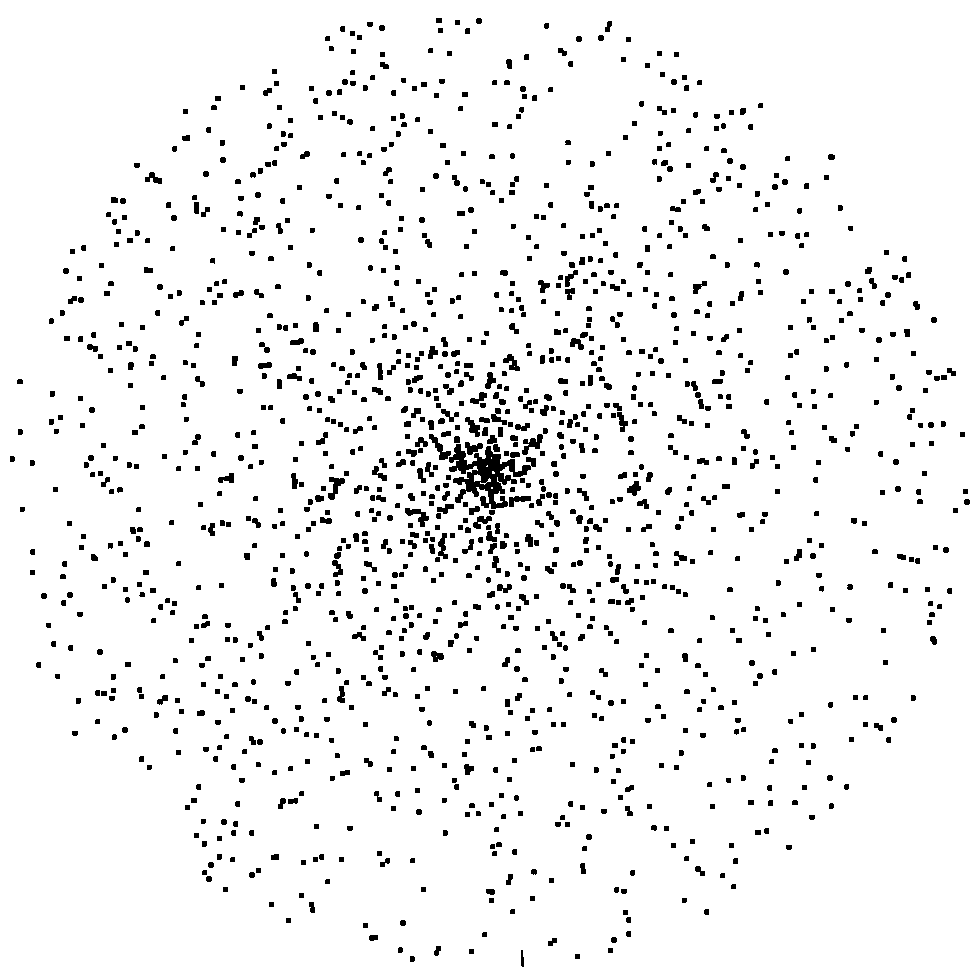
\includegraphics[width=\linewidth]{images/SCA_Extended1.png}
		\caption{$N=2000$ Einflusspunkte, zufällig in einem Ring mit dem Radius $r = 500$ verteilt.}
		\label{subfig:SCA_Extended1}
	\end{subfigure}
	\hspace{.1\textwidth}
	\begin{subfigure}[t]{.4\textwidth}
		\centering
		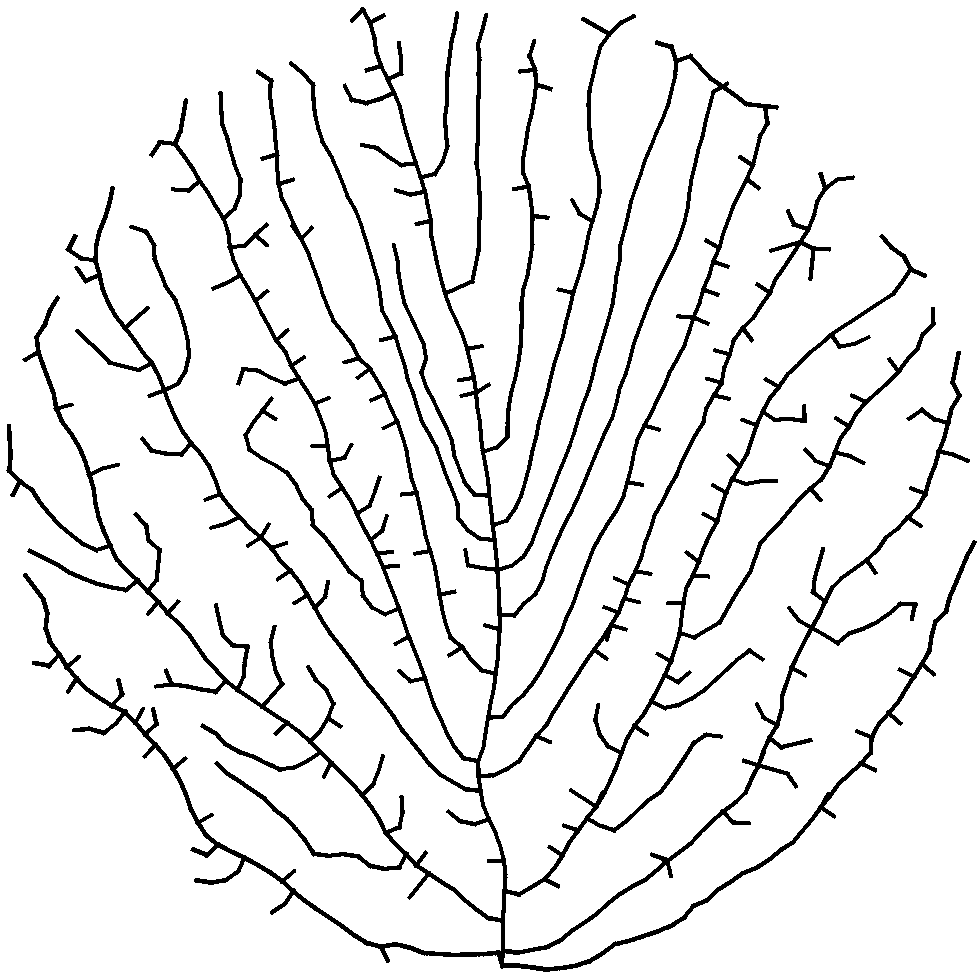
\includegraphics[width=\linewidth]{images/SCA_Extended2.png}
		\caption{Ergebnis des Space Colonization Algorithmus mit einem Einflussradius $d_i = 100$, Minimalradius $d_k = 20$, Schritteweite $D = 15$ und $\overrightarrow{T} = \overrightarrow{0}$.}
		\label{subfig:SCA_Extended2}
	\end{subfigure}
	\begin{subfigure}[t]{.4\textwidth}
		\centering
		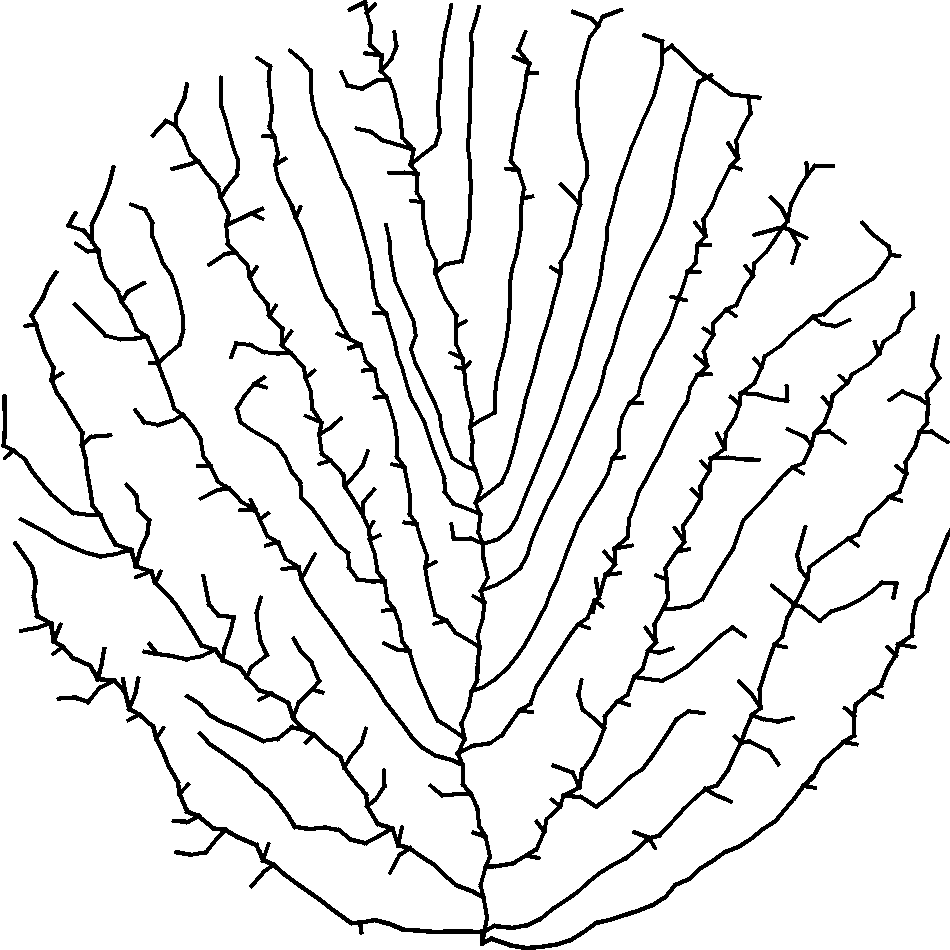
\includegraphics[width=\linewidth]{images/SCA_Extended3.png}
		\caption{Verringerung der Abzweigungswinkel.}
		\label{subfig:SCA_Extended3}
	\end{subfigure}
	\hspace{.1\textwidth}
	\begin{subfigure}[t]{.4\textwidth}
		\centering
		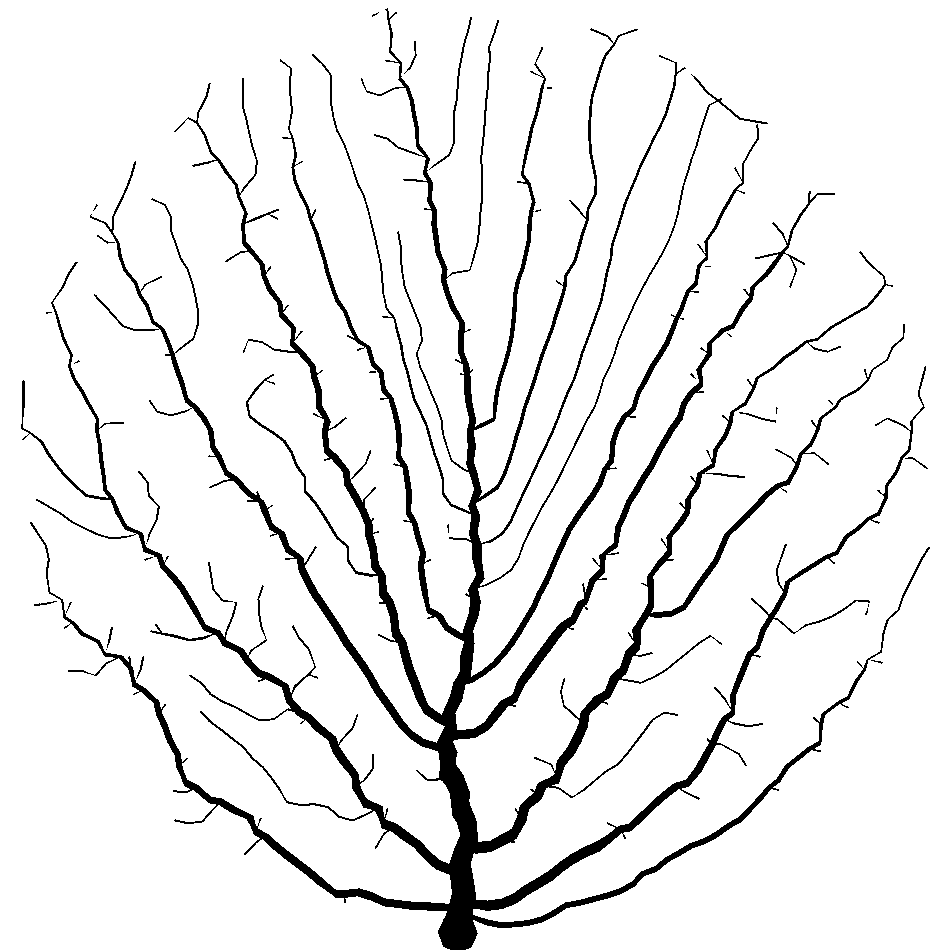
\includegraphics[width=\linewidth]{images/SCA_Extended4.png}
		\caption{Modellierung des Ergebnis mithilfe von Zylindern mit $r_0 = 1$ und $g=2$.}
		\label{subfig:SCA_Extended4}
	\end{subfigure}
	\caption{Modellierung einer zweidimensionalen Baumstruktur entsprechend der in Abschnitt \ref{sec:GenerierungBaumstrukturen} beschriebenen Schritte. Eigene Abbildungen.}
	\label{fig:SCA_Extended}
\end{figure}

\section{Erweiterungen} \label{sec:SCA_Erweiterungen}

Im Rahmen dieser Arbeit wurden die folgenden Erweiterungen des ursprünglichen Algorithmus entwickelt und implementiert.

\paragraph{Zweigtiefe}

Die Zweigtiefe $Z(v)$ eines Knotens $v \in V$ wird für Erweiterungen des Space Colonization Algorithmus und die Generierung von Modelldaten verwendet. Sie entspricht nicht der Tiefe des Knotens und berechnet sich wie folgt:
\begin{equation}
Z(v)= \begin{cases}
0 & \text{falls v die Wurzel ist} \\
Z(v') & \text{falls v' genau einen Nachfolger besitzt}\\
1 + Z(v') & \text{sonst}
\end{cases} 
\end{equation}
wobei $v'$ den Vorgänger des Knotens $v$ darstellt. Die Zweigtiefe wird direkt nach der Erstellung des Knotens berechnet und daraufhin nicht verändert. Ein Beispiel für die Bestimmung der Zweigtiefe wird in Abbildung \ref{fig:SCA_Zweigtiefe} gezeigt.

Der von Prusinkiewicz u.a. \cite{ABOP:04} beschriebene Begriff von axialen Bäumen \cite[S.21]{ABOP:04} und die zugehörige Bestimmung der Achsentiefe unterscheidet sich von der Berechnung der Zweigtiefe. Knoten können dieselbe Zweigtiefe besitzen, selbst wenn ihre Positionen keine gerade Linie bilden.

\begin{figure} [hbtp]
	\centering
	\begin{subfigure}[t]{.31\textwidth}
		\centering
		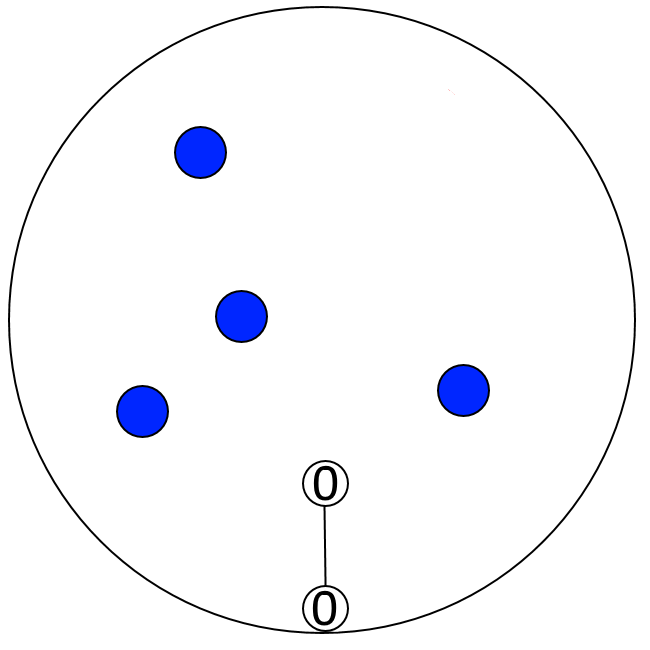
\includegraphics[width=\linewidth]{images/SCA_Zweigtiefe1.png}
		\caption{Ausgangssituation.}
		\label{subfig:SCA_Zweigtiefe1}
	\end{subfigure}
	\hspace{.01\textwidth}
	\begin{subfigure}[t]{.31\textwidth}
		\centering
		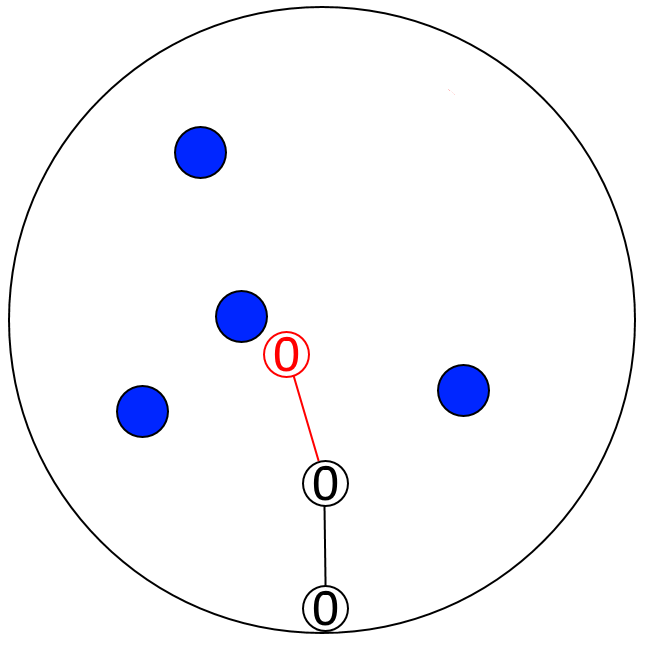
\includegraphics[width=\linewidth]{images/SCA_Zweigtiefe2.png}
		\caption{Der Vorgänger des neuen Knotens besitzt genau einen Nachfolger.}
		\label{subfig:SCA_Zweigtiefe2}
	\end{subfigure}
	\hspace{.01\textwidth}
	\begin{subfigure}[t]{.31\textwidth}
		\centering
		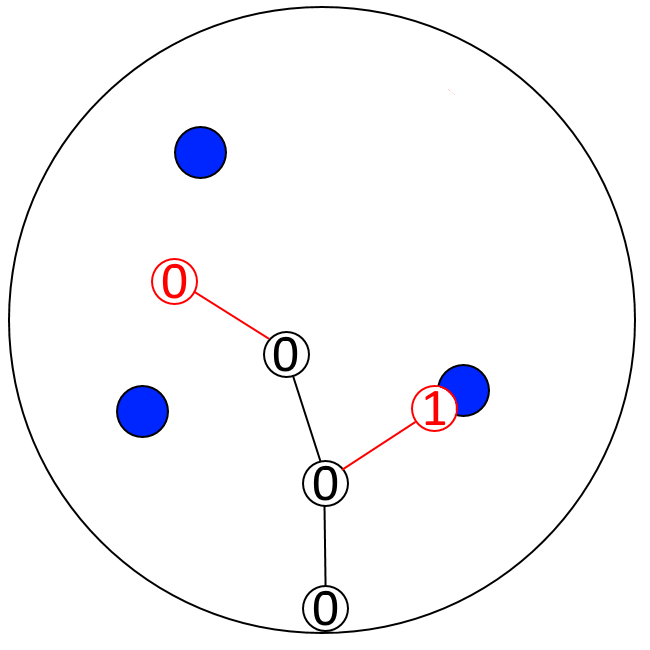
\includegraphics[width=\linewidth]{images/SCA_Zweigtiefe3.png}
		\caption{Die Zweigtiefe des rechten neuen Knotens ist um $1$ größer als der seines Vorgängers, da dieser mehr als einen Nachfolger besitzt.}
		\label{subfig:SCA_Zweigtiefe3}
	\end{subfigure}
	\caption{Darstellung der Zweigtiefen von Knotenpunkten aus Abbildung \ref{fig:SCA_Basic}. }
	\label{fig:SCA_Zweigtiefe}
\end{figure}

\paragraph{Zusätzliche Bedingungen}

Um die vom Space Colonization Algorithmus generierte Baumstruktur besser kontrollieren zu können, wurden zusätzliche Bedingungen zum Ablauf des Algorithmus hinzugefügt:
\begin{description}[labelindent]
	\item[\boldmath$max_{grad}$] Der maximale Grad der Knotenpunkte im Baum. Bevor ein neuer Knotenpunkt $v_n$ als Nachfolger eines Knotenpunkts $v$ erstellt wird, wird die Anzahl der Nachfolger von $v$ überprüft. Entspricht diese $max_{grad}$, wird der Knotenpunkt $v_n$ nicht erstellt.\\
	
	\item[\boldmath$max_{Z}$] Die maximale Zweigtiefe eines Knotens. Bevor ein neuer Knotenpunkt $v_n$ als Nachfolger eines Knotenpunkts $v$ erstellt wird, wird seine Zweigtiefe $Z(v_n)$ berechnet. Übersteigt diese $max_{Z}$, wird der Knotenpunkt $v_n$ nicht erstellt.\\
	
	\item[\boldmath$max_{NG}$] Die maximale Anzahl von Iterationen, in welchen einem Knotenpunkt kein neuer Nachfolger hinzugefügt wurde.\footnote{$NG$ steht für \glqq No Grow\grqq{} oder \glqq Did not grow\grqq, englisch für \glqq kein Wachstum\grqq.} Hat ein Knoten diesen Wert erreicht, wird er in Schritt 1 des Algorithmus \ref{alg:SCA_1} nicht weiter darauf untersucht, ob er sich innerhalb des Einflussradius eines Einflusspunktes befindet. Der Wert von $max_{NG}$ eines Knotenpunkts wird auf $0$ zurückgesetzt, falls diesem ein neuer Nachfolger hinzugefügt wurde.
	
	Durch die vorsichtige Wahl von $max_{NG}$ können Positionsvergleiche vermieden werden ohne den resultierenden Baum zu verändern.
\end{description}

\paragraph{Gewichtetes Wachstum}

Gewichtetes Wachstum ist eine Option die Schrittweite $D$ in Abhängigkeit von der Zweigtiefe zu erhöhen. Befindet sich ein Knotenpunkt auf der Zweigtiefe $0$, werden neu hinzugefügte Nachfolger im Abstand von $2 * D$ positioniert, befindet er sich auf der maximalen Zweigtiefe, werden neu hinzugefügte Nachfolger im Abstand von $D$ positioniert. Zwischen diesen beiden Zweigtiefen wird die Schrittweite linear interpoliert.

\paragraph{Kurvenreduktion} \label{par:Kurvenreduktion}
 
Kurvenreduktion in Abhängigkeit des Abzweigungswinkels ermöglicht es die Baumstruktur mithilfe einer verringerten Datenmenge darzustellen. Besitzt ein Knoten $v$ genau einen Nachfolger $v_n$ und einen Vorgänger $v'$, werden die zwei Richtungsvektoren zwischen $v'$ und $v$ sowie $v$ und $v_n$ berechnet:
\begin{equation}
\overrightarrow{R_1} = \dfrac{\overrightarrow{p_v} - \overrightarrow{p_{v'}}}{\lVert\overrightarrow{p_v} - \overrightarrow{p_{v'}} \rVert} \text{ und } \overrightarrow{R_2} = \dfrac{\overrightarrow{p_{v_n}} - \overrightarrow{p_{v}}}{\lVert \overrightarrow{p_{v_n}} - \overrightarrow{p_{v}} \rVert}
\end{equation}

Übersteigt das Skalarprodukt $\langle \overrightarrow{R_1}, \overrightarrow{R_2} \rangle$ einen festgelegten Maximalwert $max_K$ zwischen $0$ und $1$, wird $v$ aus dem Baum entfernt. $v_n$ wird zum Nachfolger von $v'$ und $v'$ zum Vorgänger von $v_n$. 

Die Kurvenreduktion kann auch auf Bäume angewendet werden, welche wie in Abschnitt \ref{sec:LS_Baumstrukturen} beschrieben durch eine Turtle-Interpretation aufgebaut wurden.
\chapter{Implementierung}


Im folgenden Kapitel wird die Implementierung der Vorgehen innerhalb des Frameworks der Unreal Engine 4 behandelt. Die Baumrepräsentation enthält Daten, die von den L-System und Space Colonization Implementierungen generiert werden. Diese Daten werden an das Modellgenerierungssystem übergeben, welches die Modelldaten für eine grafische Darstellung in der Unreal Engine 4 produziert.


\section{Baumrepräsentation}

Sowohl L-Systeme als auch der Space Colonization Algorithmus generieren einen graphentheoretischen Baum, auf dessen Grundlage die Modellgenerierung durchgeführt wird. Die implementierte Baumrepräsentation kann daher von beiden Systemen verwendet werden und ermöglicht es, diese mit demselben Modellgenerierungssystem zu visualisieren.

Der Baum wird durch eine Datenklasse repräsentiert, jedes Objekt dieser Klasse beschreibt einen Knoten sowie die Kante, welche vom Vorgänger zu dem Knoten führt. Die Datenklasse bietet Zugriff auf die folgenden Informationen:

\begin{description}
	\item \textbf{Vorgänger und Nachfolger:} Mithilfe eines Verweises auf den Vorgänger und eine Liste der Nachfolger eines Knotens kann der Baum-Graph vollständig repräsentiert werden. Weiterhin ermöglicht dies die Implementierung einer Reihe von rekursiven Funktionen zur Anpassung von Modelldaten.\\
	
	\item \textbf{Modell-Daten:} Kanten werden, wie in Abschnitt \ref{subsec:ZylinderMeshes} beschrieben, mithilfe von Zylindern visualisiert. Um die Generierung von Modelldaten zu vereinfachen, bietet die Datenklasse Zugriff auf Start- und Endposition, Start- und Endradius, Start- und Endnormale sowie einen Rotationswinkel. 
	
	Des Weiteren wird die Zweigtiefe des repräsentierten Knoten gespeichert.\\
	
	\item \textbf{Wachstums-Daten:} Die Wachstums-Daten bestehen aus einer Wachstumsrichtung, einem Einfluss-Zähler und dem \glqq Kein Wachstum\grqq-Zähler ($NG$-Counter), welche für den Ablauf des Space Colonization Algorithmus benötigt werden.	
\end{description}

Ein Objekt der Datenklasse kann als Astsegment eines biologischen Baumes angesehen werden und wird durch das Modellgenerierungssystem als solches visualisiert. Im Folgenden wird der Begriff \glqq Astsegment\grqq{} verwendet, um ein Objekt der Datenklasse der Baumrepräsentation zu bezeichnen.

\section{L-Systeme}

Die Implementierung der Funktionsweise von L-Systemen wird durch einen Unreal-Actor verwirklicht, der im Level platziert werden kann. Nach Start des Levels wird das angegebene Axiom anhand der Produktionsregeln abgeleitet und die sich ergebende Zeichenkette von der Turtle-Implementierung interpretiert.

\subsection{Parameter}

Dem L-System-Actor werden die folgenden Parameter über die Editor-UI übergeben:

\begin{description}
	\item \textbf{Anzahl der Ableitungen:} Die Anzahl der Ableitungen in $\mathbb{N}^+$, welche auf dem Axiom durchgeführt werden. \\
	
	\item \textbf{Axiom:} Das Axiom in Form einer Zeichenkette. \\
	
	\item \textbf{Konstanten:} Eine Konstante besteht aus der Angabe eines Identifikationssymbols und eines Wertes in $\mathbb{R}$. Konstanten können im Axiom und in den Nachfolgern der Produktionen verwendet werden.\\	
	
	\item \textbf{Produktionen:} Jede Produktion besteht aus Angabe eines Vorgängers, eine Liste von Parametern und einem Nachfolger. Der Vorgänger und jeder Parameter entspricht einem einzelnen Symbol, der Nachfolger wird als Zeichenkette eingetragen. Die Parametersymbole können nur innerhalb des Nachfolgers verwendet werden. Der Vorgänger und die Liste der Parameter bilden das parametrische Wort, welches bei einer Ableitung durch den Nachfolger ersetzt wird. \\
	
	\item \textbf{Tropismus:} Der Einfluss von Tropismus in Form eines dreidimensionalen Vektors und eines Biegsamkeitsfaktors.
\end{description}
\begin{figure} [hbtp]
	\centering
	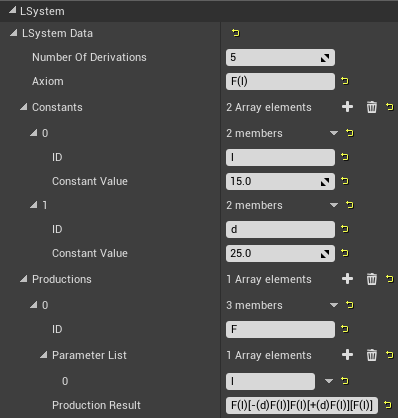
\includegraphics[height=0.4\textheight]{images/LS_ExampleUE4UI.png}
	\caption{Ein Beispiel für die Angabe des L-Systems aus Gleichung \ref{eq:ProdBranching2} mit der resultierenden Baumstruktur aus Abbildung \ref{fig:Branching2L15D25}.}
	\label{fig:LS_ExampleUE4UI}
\end{figure}
Für das Axiom und die Produktionen gelten die in Kapitel \ref{ch:LSysteme} festgelegten Regeln für die Definition von L-Systemen. Weiterhin gelten die Regeln für die Angabe von arithmetischen Operationen. Die Verwendung von Klammern ist jedoch auf die Angabe von Parametern eines parametrischen Wortes beschränkt, ihre Verwendung zur Beeinflussung der Auswertungsreihenfolge eines arithmetischen Ausdrucks wird nicht unterstützt.

Ein Beispiel für die korrekte Eingabe eines L-Systems über die Editor-UI wird in Abbildung \ref{fig:LS_ExampleUE4UI} gezeigt.

\subsection{Ableitung}

Zu Anfang der Erstellung des L-System-Actors werden alle Konstantensymbole im Axiom und den Produktionen durch die Konstantenwerte ersetzt. 

Die Implementierung arbeitet durchgehend auf derselben Zeichenkette, angefangen mit dem Axiom. In jeder Ableitung werden die in den Produktionsregeln definierten parametrischen Wörter durch die angegebenen Nachfolger ersetzt.

Nachdem die vorgegebene Anzahl von Ableitungen durchgeführt wurde, wird die resultierende Zeichenkette an die Turtle-Implementierung weiter gegeben.

\subsection{Turtle Interpretation} \label{subsec:TurtleInterpretationImplementation}

Der Turtle-Implementierung wird die aus den Ableitungen resultierende Zeichenkette übergeben. Diese wird daraufhin sequentiell abgearbeitet und entsprechend den in Abschnitt \ref{sec:LS_Baumstrukturen} vorgestellten Konzepten interpretiert. Der resultierende Baum wird für die Konstruktion des Modells an das Modellgenerierungssystem weitergegeben.

\section{Space Colonization Algorithmus}

Die Implementierung einer Space-Colonization-Baumstruktur stellt sich aus der Platzierung von mindestens einem Actor für die Repräsentation des Einflussbereichs und einem Actor für die Umsetzung des Algorithmus zusammen.

\subsection{Einflussbereiche}

Durch die Platzierung von Einflussbereich-Actors kann die Verteilung von Einflusspunkten mithilfe des Unreal-Editors angepasst werden. Es sind derzeit zwei Formen von Einflussbereichen wählbar: Eine Kugel- und eine Zylinderform. Die Kugelform erfordert die Angabe eines Kugelradius während die Zylinderform durch Höhe und Radius beschrieben wird. 

Einem Space-Colonization-Actor können mehrere Einflussbereiche zugeordnet werden, um eine bestimmte Baumstruktur zu formen. Jeder Einflussbereich-Actor wird weiterhin in einem vorgegebenen Abstand zum Space-Colonization-Actor platziert.

Dem Einflussbereich muss eine positive Anzahl von zu generierenden Einflusspunkten und ein Random-Seed Wert übergeben werden. Ein Random-Seed ist ein Wert, der von einem Zufallsgenerator verwendet wird, um eine Folge von zufälligen Zahlen zu generieren. Bei Verwendung desselben Random-Seeds wird dieselbe Folge von Zufallszahlen erstellt, was eine Kontrolle über Generierung ermöglicht. Somit wird, wenn auch alle anderen Parameter übereinstimmen, mit demselben Random-Seed Wert dieselbe Baumstruktur aufgebaut. 

\subsection{Parameter}

Dem Space-Colonization-Actor werden Parameter des ursprünglichen Algorithmus sowie die Eingaben für in Abschnitt \ref{sec:SCA_Erweiterungen} besprochene Erweiterungen über das Editor-UI übergeben. Zu den ursprünglichen Parametern gehören der Minimalradius, Einflussradius, Schrittweite, ein Tropismusvektor sowie die Anzahl der durchzuführenden Iterationen. Zu den erweiterten Parametern gehören der maximale Grad, die maximale Zweigtiefe, die maximale Anzahl von \glqq Kein Wachstum\grqq{}-Iterationen und eine Abfrage, ob gewichtetes Wachstum durchgeführt werden soll.

Weiterhin müssen die zugeordneten Einflussbereich-Actors angegeben werden -- damit der Algorithmus durchgeführt werden kann, muss mindestens einer dieser Actors mit mindestens einem Einflusspunkt eingetragen werden.

\subsection{Ablauf des Algorithmus}

Die Einflusspunkte aller dem Space-Colonization-Actor zugeordneten Einflussbereiche werden diesem zu Beginn der Baum-Generierung übergeben. Daraufhin wird ein Baum entsprechend der in Abschnitt \ref{sec:GenerierungBaumstrukturen} und Abschnitt \ref{sec:SCA_Erweiterungen} vorgestellten Konzepte aufgebaut und für die Konstruktion des Modells an das Modellgenerierungssystem weitergegeben.

\section{Modellgenerierung} \label{sec:Modellgenerierung}

Das Modellgenerierungssystem erhält einen graphentheoretischen Baum von L-System- und Space-Colonization-Actors und generiert ein dreidimensionales Mesh (engl. für Polygonnetz) in der von dem Framework geforderten Form. Das Mesh entspricht der Visualisierung der Kanten des Baums in Form von Zylindern und simuliert dadurch vereinfacht die Aststruktur eines biologischen Baumes. \cite[Abschn. 2]{SpaceColonizationAlgorithm:07} 

\subsection{Procedural Mesh Component}

Die Procedural Mesh Component ist eine Komponente der Unreal Engine, welche die Darstellung von prozedural generierten Polygonnetzen zulässt. Ein Vertex ist ein Punkt in einem Polygonnetz mit zur Visualisierung benötigten Informationen. Der Komponente werden Vertexdaten in Form von Listen aus Positions-, Normalen-, Tangenten-, Textur- und Indexdaten übergeben. Das Grafiksystem der Unreal Engine ist daraufhin in der Lage, die Komponente als dreidimensionales Modell im Level darzustellen. \cite{ProceduralMeshComponent:15} Die Vertexdaten werden, basierend auf dem übergebenen Baum und den Parametern, vom Modellgenerierungssytem erstellt.

Jedem L-System-Actor und Space-Colonization-Actor ist eine Procedural Mesh Component zugeordnet.

\subsection{Parameter} \label{subsec:Modellgenerierung_Parameter}

Dem Modellgenerierungssystem werden die folgenden Parameter über die Editor-UI übergeben:

\begin{description}
	\item \textbf{Radius-Daten:} Dies beinhaltet den Blattradius, den Radiuswachstumswert, den Stammbreitenmultiplikator und die Abfrage, ob Radiusberechnungen durchgeführt werden sollen. \\
	
	\item \textbf{Genauigkeit:} Dies beinhaltet die minimale und maximale Anzahl von Zylindersektionen sowie den Kurvenreduktionswert. \\
	
	\item \textbf{Sonstiges:} Weiterhin wird ein Startrotationswinkel, ein Material und eine Abfrage, ob ein fraktales Mesh erstellt werden soll, übergeben. Ein Material beinhaltet Textur- und Shaderinformationen und ist für die Oberflächenbeschaffenheit des generierten Modells verantwortlich.
\end{description}

\subsection{Operationen auf dem Baum}

Folgende Operationen werden vor Beginn der Modelldatengenerierung auf dem graphentheoretischen Baum durchgeführt:

\begin{description}
	\item \textbf{Kurvenreduktion:} Die Kurvenreduktion wird, beginnend mit dem Wurzel-Astsegment des Baums, rekursiv ausgeführt. In jedem Schritt wird überprüft ob das aktuelle Astsegment entsprechend der Beschreibung in Paragraph \ref{par:Kurvenreduktion} entfernt werden kann. Falls nicht, wird die Kurvenreduktion auf allen Nachfolgern des aktuellen Astsegment durchgeführt. Die Rekursion bricht ab, falls ein Astsegment keine Nachfolger besitzt.
	
	Der Parameter \glqq Kurvenreduktionswert\grqq{} entspricht dem Maximalwert des Skalarprodukts $max_K$.\\
	
	\item \textbf{Radiusberechnung:} Der Endradius jedes Astsegments wird, beginnend mit dem Wurzel-Astsegment des Baums, rekursiv anhand von Gleichung \ref{eq:Radiusberechnung} berechnet. Der Parameter \glqq Blattradius\grqq{} entspricht $r_0$ und der \glqq Radiuswachstumswert\grqq{} entspricht $g$. 
	
	Der Startradius jedes Astsegments wird auf den Wert des Endradius seines Vorgängers gesetzt. Da das Wurzel-Astsegment keinen Vorgänger besitzt, wird der Startradius aus der Multiplikation des Stammbreitenmultiplikators mit dem Endradius des Objekts bestimmt.\\
	
	\item \textbf{Normalenberechnung:} Normalen werden für die Berechnung der Modelldaten benötigt. Die Endnormale $\overrightarrow{n_{e}}$ jedes Astsegments wird mithilfe der Startposition $\overrightarrow{p_{s}}$ und Endposition $\overrightarrow{p_{e}}$ sowie seiner Startnormale $\overrightarrow{n_{s}}$ wie folgt berechnet:
	\begin{equation}
		\overrightarrow{n_{e}} = \dfrac{(\overrightarrow{p_{e}} - \overrightarrow{p_{s}}) + \overrightarrow{n_{s}}}{\lVert (\overrightarrow{p_{e}} - \overrightarrow{p_{s}}) + \overrightarrow{n_{s}} \rVert}
	\end{equation}
	Die Startnormale entspricht der Endnormale des Vorgängers, im Falle des Wurzel-Astsegments entspricht die Startnormale $\overrightarrow{n_s} = \overrightarrow{p_{e}} - \overrightarrow{p_{e}}$. \\
	
	
	\item \textbf{Verringerung der Abzweigungswinkel:} Die Nachfolger jedes Astsegments werden, entsprechend der Beschreibung in Paragraph \ref{par:VerringerungAbzweigungswinkel}, einander angenähert. Die Verringerung der Abzweigungswinkel wird nur bei durch Space-Colonization-Actors generierten Bäumen durchgeführt.
\end{description}


\subsection{Generierung der Zylinder-Meshes} \label{subsec:ZylinderMeshes}

Moderne Grafik-APIs stellen dreidimensionale Modelle in Form von geometrischen Primitiven -- in diesem Fall in Form von Dreiecken -- dar. Je drei Vertizes bilden ein Dreieck, dessen Oberfläche mithilfe eines übergebenen Materials gefärbt wird.

Die Vertizes bestehen zusätzlich zu ihren Positionen aus :

\begin{description}
	\item \textbf{Normalenvektoren}, welche die Richtung darstellen, von der aus das Dreieck sichtbar ist und für Beleuchtungsberechnungen benötigt werden. \cite{ModelingByNumbers1A:13} 
	\item \textbf{Tangentenvektoren}, welche orthogonal zu den Normalenvektoren stehen und für erweiterte Beleuchtungsberechnungen benötigt werden. \cite{ModelingByNumbers1A:13} 
\end{description}

Mithilfe dieser Informationen werden zusätzlich Texturkoordinaten, welche für das korrekte Auftragen von Texturen auf das Modell benötigt werden, und Indexdaten, welche für die Darstellung des Polygonnetzes benötigt werden, berechnet. Diese Berechnungen werden in den folgenden Paragraphen der Übersicht halber weggelassen.

Der Mantel eines Zylinder kann nun durch die Verbindung von zwei Kreisen generiert werden. 

\paragraph{Berechnung der Vertizes auf einem Kreis}

Da ein Kreis theoretisch aus unendlich vielen Punkten besteht, muss eine gewisse Genauigkeit bei der Darstellung von runden Modellen festgelegt werden -- ein Kreis wird aus einer zuvor definierten Anzahl von Segmenten generiert. Mithilfe eines Mittelpunkts $\overrightarrow{c}$ und  einem Radius $r$ kann ein Kreis im zweidimensionalen Raum beschrieben werden. Die Vertexpositionen $\overrightarrow{v_i}$ werden wie folgt berechnet:

\begin{equation}
	\overrightarrow{v_i} =\overrightarrow{c} + r * \begin{pmatrix}
	cos(d)\\
	sin(d)\\
	0
	\end{pmatrix}
	\text{ mit } d = rot_z + i * \frac{360\degree}{n} \text{ und } i = 0 ... (n-1)
\end{equation}
\cite{ModelingByNumbersZylindersA:13}

wobei $n$ der Anzahl der Segmente und $rot_z$ einem Startrotationswinkel entspricht.

Mithilfe der Kreisnormalen $\overrightarrow{n_k}$, die orthogonal zur Kreisebene steht und des Kreismittelpunkts $\overrightarrow{c}$ kann die Kreisebene beschrieben werden, auf welcher die Vertizes zu generieren sind. Eine Vertexposition $\overrightarrow{v_i}$ muss um den Kreismittelpunkt rotiert werden, um auf der Kreisebene zu liegen, wobei Rotationsachse $\overrightarrow{R}$ und Rotationswinkel $\alpha$ wie folgt berechnet werden:
\begin{equation}
\overrightarrow{R} = \dfrac{(\overrightarrow{v_i} - \overrightarrow{c}) \times \overrightarrow{n_k}}{\lVert (\overrightarrow{v_i} - \overrightarrow{c}) \times \overrightarrow{n_k} \rVert}
\end{equation}

\begin{equation}
\alpha = arccos(\langle \overrightarrow{n_k}, \overrightarrow{z} \rangle) \text{ mit } \overrightarrow{z} = \begin{pmatrix}
0\\
0\\
1
\end{pmatrix}
\end{equation}
 wobei $arccos$ dem Arkuskosinus entspricht. \cite{RotationBetweenVectors:16} 
 Die rotierte Vertexposition $\overrightarrow{v}$ ermöglicht die Berechnung der Vertexnormalen $\overrightarrow{n_v}$ und Vertextangente $\overrightarrow{t_v}$:
 
 \begin{equation}
	 \overrightarrow{n_v} = \dfrac{\overrightarrow{v} - \overrightarrow{c}}{\lVert \overrightarrow{v} - \overrightarrow{c} \rVert} \text{ und } \overrightarrow{t_v} = \overrightarrow{n_v} \times \overrightarrow{n_k}
 \end{equation}
\begin{figure} [hbtp]
	\centering
	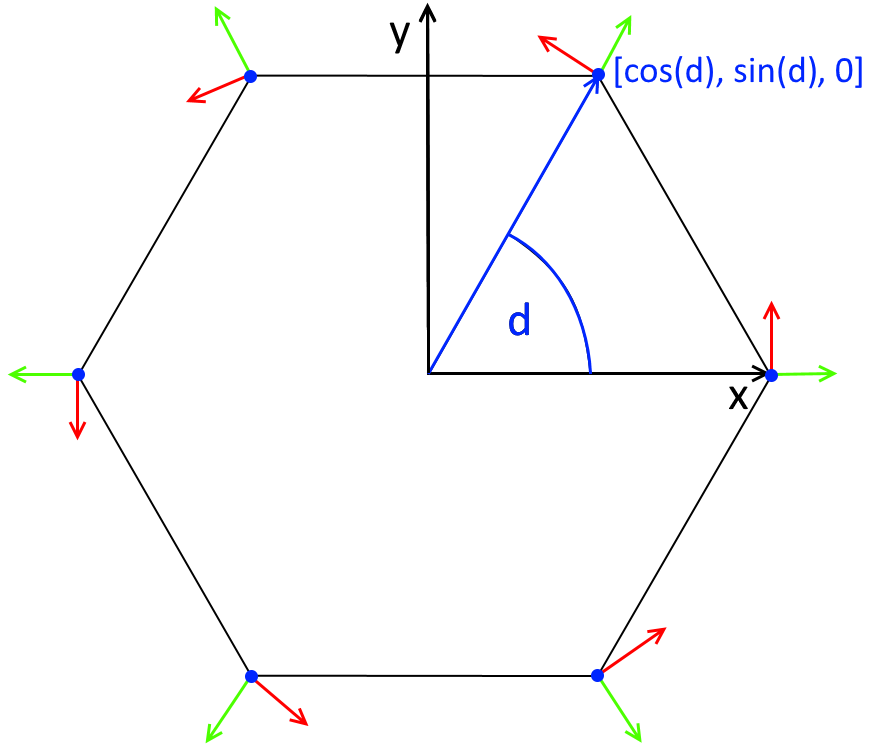
\includegraphics[height=0.25\textheight]{images/Ring6Sections.png}
	\caption{Beispiel für die Berechnung von Vertexpositionen auf einem Einheitskreis mit einer Genauigkeit von sechs Segmenten. $d = \frac{360\degree}{6} = 60 \degree$. Die blauen Punkte entsprechen den Positionen, die grünen Pfeile den Normalen und die roten Pfeile den Tangenten der Vertizes. Eigene Abbildung.}
	\label{fig:Ring6Sections}
\end{figure}
\paragraph{Verbindung der Kreise}
Um den Zylindermantel eines Astsegments zu bilden, werden zwei Kreise mithilfe der Start- und Enddaten des Objekts generiert. Jedes Segment eines Kreises wird mit dem entsprechenden Segment des anderen Kreises verbunden und bildet dadurch ein Zylindersegment. Ein Zylindersegment entspricht somit einem Rechteck. Da das Modell jedoch Dreiecksdaten benötigt, wird jedes Rechteck, wie in Abbildung \ref{subfig:Zylinder10SegmenteWireframe} dargestellt, aus zwei Dreiecken gebildet. \cite{ModelingByNumbersZylindersA:13}
\begin{figure} [hbtp]
\centering
\begin{subfigure}[t]{.4\textwidth}
	\centering
	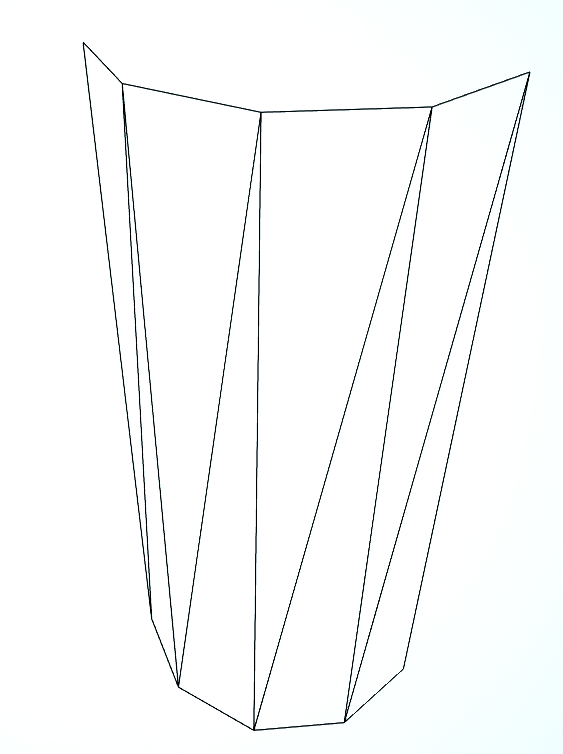
\includegraphics[height=.75\linewidth]{images/Zylinder10SegmenteWireframe.png}
	\caption{Darstellung der Dreiecke, welche bei der Verbindung der Kreise entstehen.}
	\label{subfig:Zylinder10SegmenteWireframe}
\end{subfigure}
\hspace{.1\textwidth}
\begin{subfigure}[t]{.4\textwidth}
	\centering
	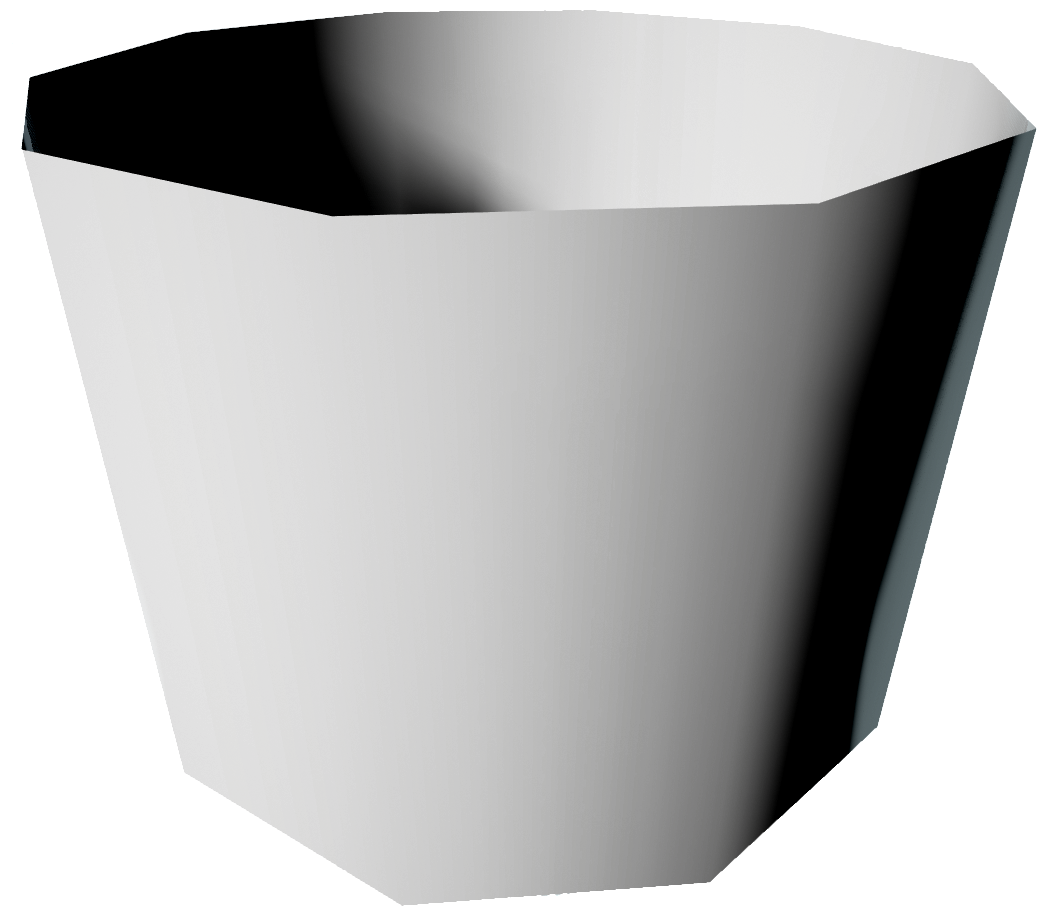
\includegraphics[height=.75\linewidth]{images/Zylinder10SegmenteOpaque.png}
	\caption{Gefärbte Dreiecke mit Beleuchtungsberechnung.}
	\label{subfig:Zylinder10SegmenteOpaque}
\end{subfigure}
\caption{Verbindung zweier Kreise zu einem Zylindermantel. Eigene Abbildungen.}
\label{fig:Zylinder10Segmente}
\end{figure}

Wird jedes Astsegment durch die Verbindung von genau zwei Kreisen dargestellt, führt dies zu der Generierung redundanter Vertexdaten. Die Enddaten eines Astsegments und die Startdaten seines Nachfolgers entsprechen einander, da die daraus generierten Kreis-Vertizes genau aufeinander liegen. Anstatt nun vier Kreise für die Generierung zweier Zylinder zu verwenden, können die Vertizes des verbindenden Kreises wiederverwendet werden -- es genügen drei Kreise für die Generierung zweier Zylinder.

Die Verbindung der Modelldaten kann für alle Astsegmente durchgeführt werden, deren Nachfolger dieselbe Zweigtiefe besitzen und somit eine Folge von zusammenhängenden Zylindermodellen bilden. Für einen Nachfolger mit einer sich unterscheidenden Zweigtiefe wird eine neue Folge von zusammenhängenden Zylindermodellen begonnen. \cite{ModelingByNumbersZylindersA:13}

Ein Beispiel für die Generierung zweier Zylinder mithilfe von drei Kreisen wird in Abbildung \ref{subfig:MultiZylinder10SegmenteWireframe} dargestellt.

\begin{figure} [hbtp]
	\centering
	\begin{subfigure}[t]{.4\textwidth}
		\centering
		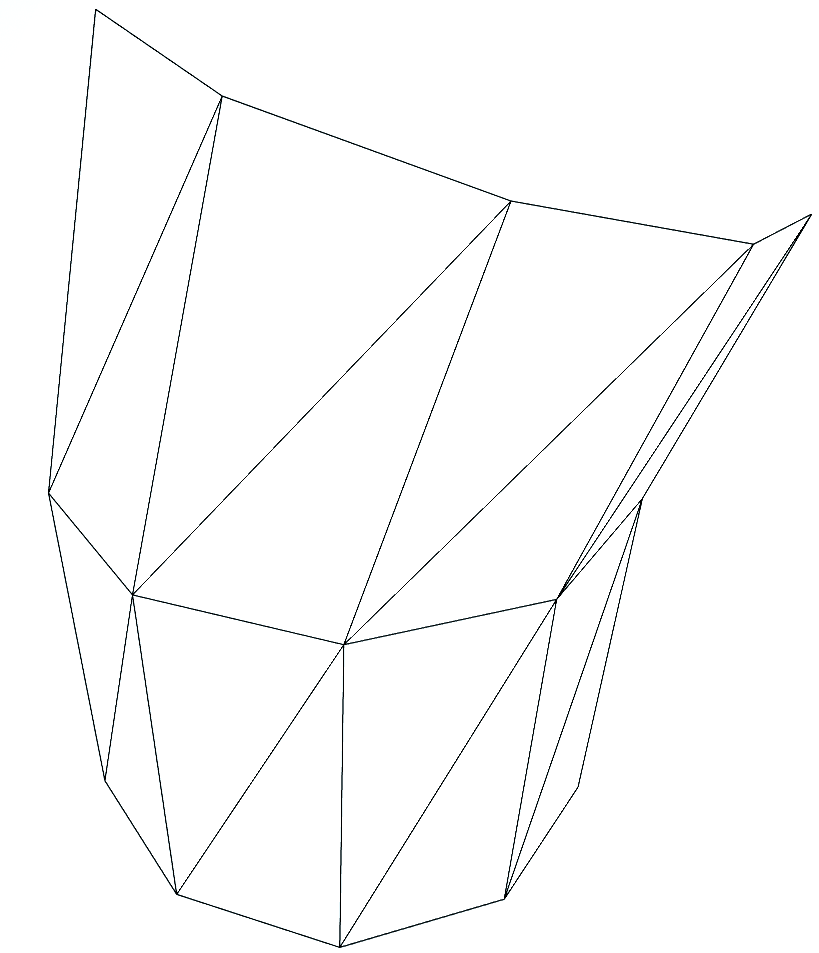
\includegraphics[height=\linewidth]{images/MultiZylinder10SegmenteWireframe.png}
		\caption{Darstellung der Dreiecke, welche bei der Verbindung der Kreise entstehen.}
		\label{subfig:MultiZylinder10SegmenteWireframe}
	\end{subfigure}
	\hspace{.1\textwidth}
	\begin{subfigure}[t]{.4\textwidth}
		\centering
		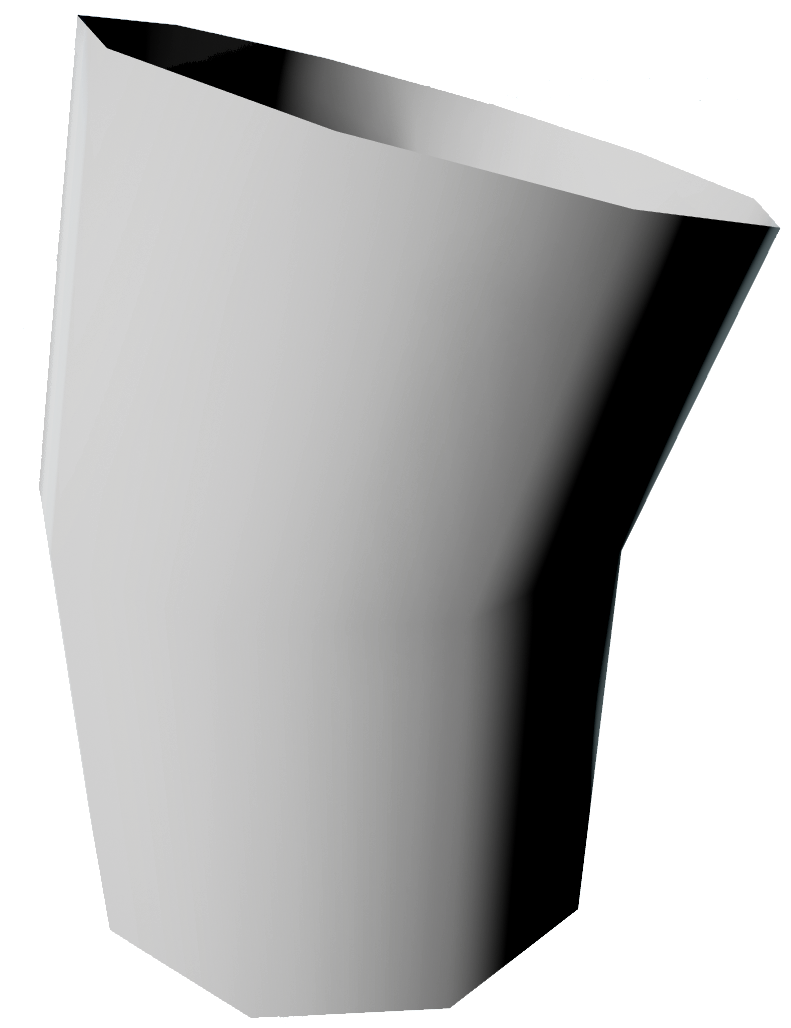
\includegraphics[height=\linewidth]{images/MultiZylinder10SegmenteOpaque.png}
		\caption{Gefärbte Dreiecke mit Beleuchtungsberechnung.}
		\label{subfig:MultiZylinder10SegmenteOpaque}
	\end{subfigure}
	\caption{Verbindung dreier Kreise zu einer Folge zusammenhängender Zylindermodelle. Eigene Abbildungen.}
	\label{fig:MultiZylinder10Segmente}
\end{figure}





\chapter{Ergebnisse}
In diesem Kapitel werden die Ergebnisse vorgestellt, die mithilfe der Implementierungen von L-Systemen und dem Space-Colonization Algorithmus produziert wurden. Es bietet sich an in vielen Fällen biologisch motivierte Begriffe zu verwenden -- beispielsweise Kanten als Äste oder Zweige zu bezeichnen -- um eine Verbindung zwischen visueller Repräsentation und graphentheoretischem Hintergrund zu schaffen.

\section{L-System-Actor}
L-Systeme ermöglichen es mithilfe bestimmter Produktionsregeln realitätsnahe Baumstrukturen zu generieren. Im Folgenden werden verschiedene natürliche Wachstumsarten mithilfe der L-System Implementierung nachgeahmt und visualisiert.
\subsection{Monopodiales Wachstum}
Ein biologischer Baum mit monopodialem Wachstumsverhalten bildet einen Hauptstamm, der stets weiterwächst, mit davon abzweigenden Nebenästen. \cite[S.14]{Deussen:05} Ein Beispiel für ein solches Wachstum ist das folgende L-System:

\begin{equation}
\begin{array}{llll}
\omega & : F(s)A(100) \\
p_1 & : A(l) &\rightarrow& F(l)\text{ }[\&(a1)\text{ }B(l)]\text{ }/(d1)\text{ }A(l*r1) \\
p_2 &  : B(l) &\rightarrow& F(l)\text{ }[-(a2)\text{ }B(l*r2)]\text{ }/(d2)\text{ }B(l*r2)
\end{array}
\label{eq:ProdMonopodial}
\end{equation} 
\cite[S.56]{ABOP:04}

Die Produktionsregel $p_1$ produziert den Hauptstamm, welcher in jeder Ableitung verlängert wird und einen Nebenast produziert, der anhand von $p_2$ ebenfalls entlang einer Hauptachse weiterwächst und weitere Nebenäste produziert. $a_1$ und $a_2$ entsprechen den Abzweigungswinkeln neuer Äste von der Hauptachse, während die Winkel $d_1$ und $d_2$ die Rotation um die Hauptachse beschreiben, bevor ein neuer Nebenast produziert wird. $r_1$ und $r_2$ entsprechen Faktoren, welche das Wachstum eines Astes pro Ableitung verkürzen, falls der Wert unter $1$ liegt und verlängern, falls der Wert über $1$ liegt. Die Variable $s$ beschreibt die Länge des Stammes, bevor das Wachstum beginnt. \cite[S.57]{ABOP:04}

Abbildung \ref{fig:LS_Monopodial} zeigt Beispiele für monopodiale Baumstrukturen, Tabelle \ref{tab:LS_Monopodial} die verwendeten Konstantenwerte. Es findet kein Einfluss durch Tropismus statt.
\begin{center}
	\begin{tabulary}{\textwidth}{|C|C|C|C|C|C|C|C|C|}
		\hline 
		Abbildung & $n$ & $a_1$ & $a_2$ & $r_1$ & $r_2$ & $d_1$ & $d_2$ & $s$ \\ 
		\hline 
		a & 11 & 45.0 & 35.0 & 1.05 & 0.9 & 137.5 & 70.0 & 100.0 \\ 
		\hline 
		b & 11 & 60.0 & 20.0 & 1.05 & 0.9 & 137.5 & 70.0 & 100.0 \\ 
		\hline 
		c & 11 & 45.0 & 35.0 & 0.95 & 0.9 & 137.5 & 70.0 & 350.0 \\ 
		\hline 
		d & 11 & 77.0 & -37.0 & 1.05 & 0.85 & 137.5 & -70.0 & 200.0 \\ 
		\hline 
	\end{tabulary} 
	\captionof{table}{Konstantenwerte der in Abbildung \ref{fig:LS_Monopodial} dargestellten monopodialen Baumstrukturen.} 
	\label{tab:LS_Monopodial}
\end{center}


\begin{figure} [hbtp]
	\centering
	\begin{subfigure}[t]{.45\textwidth}
		\centering
		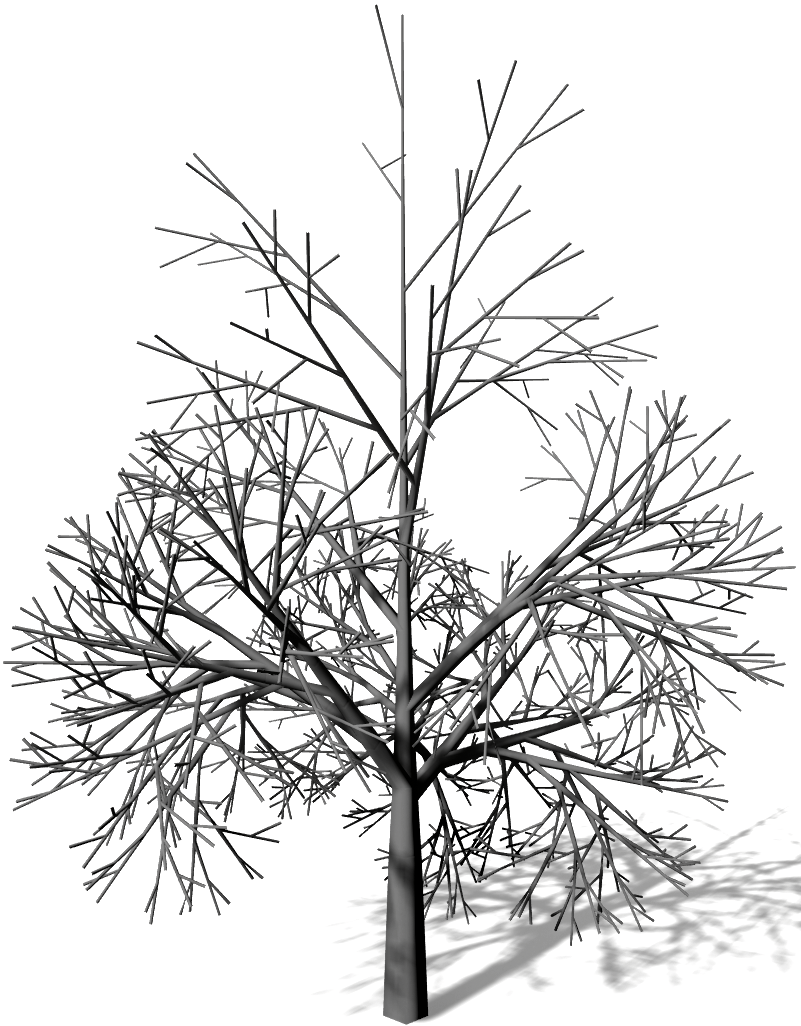
\includegraphics[height=.21\textheight]{images/LS_Monopodial_1.png}
		\caption{}
		\label{subfig:LS_Monopodial_1}
	\end{subfigure}
	\begin{subfigure}[t]{.45\textwidth}
		\centering
		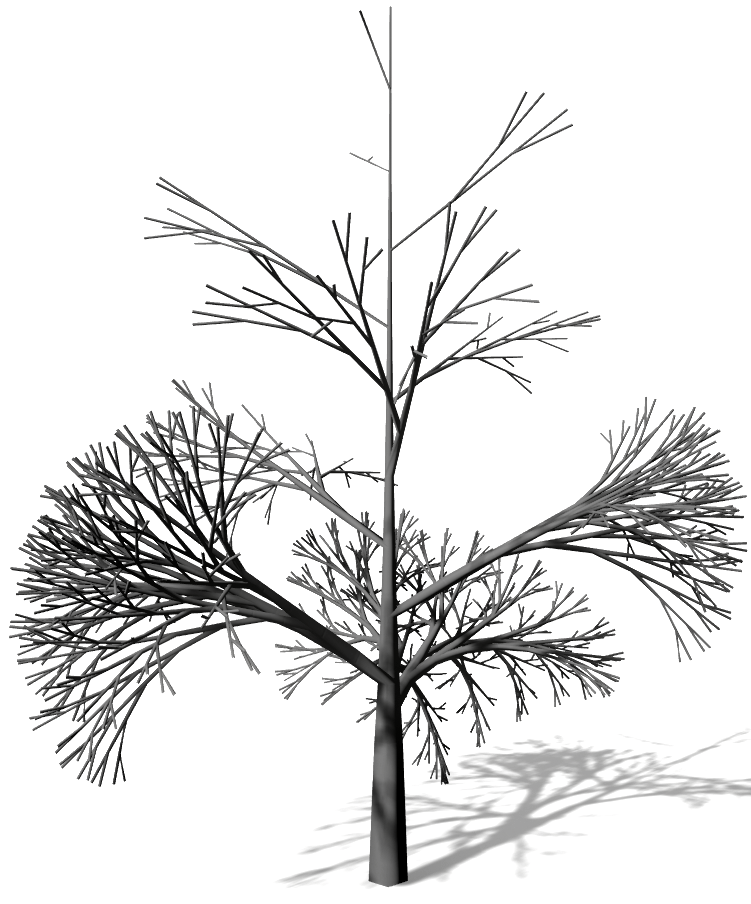
\includegraphics[height=.21\textheight]{images/LS_Monopodial_2.png}
		\caption{}
		\label{subfig:LS_Monopodial_2}
	\end{subfigure}	
	\begin{subfigure}[t]{.45\textwidth}
		\centering
		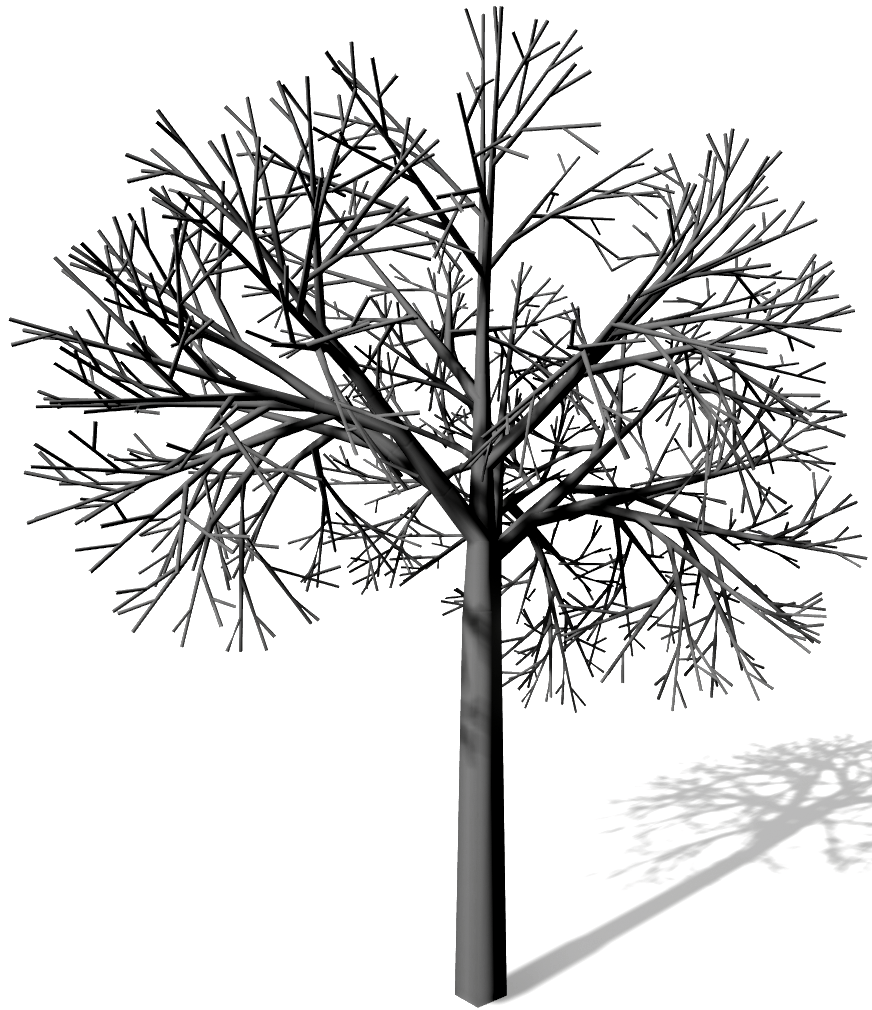
\includegraphics[height=.21\textheight]{images/LS_Monopodial_3.png}
		\caption{}
		\label{subfig:LS_Monopodial_3}
	\end{subfigure}
	\begin{subfigure}[t]{.45\textwidth}
		\centering
		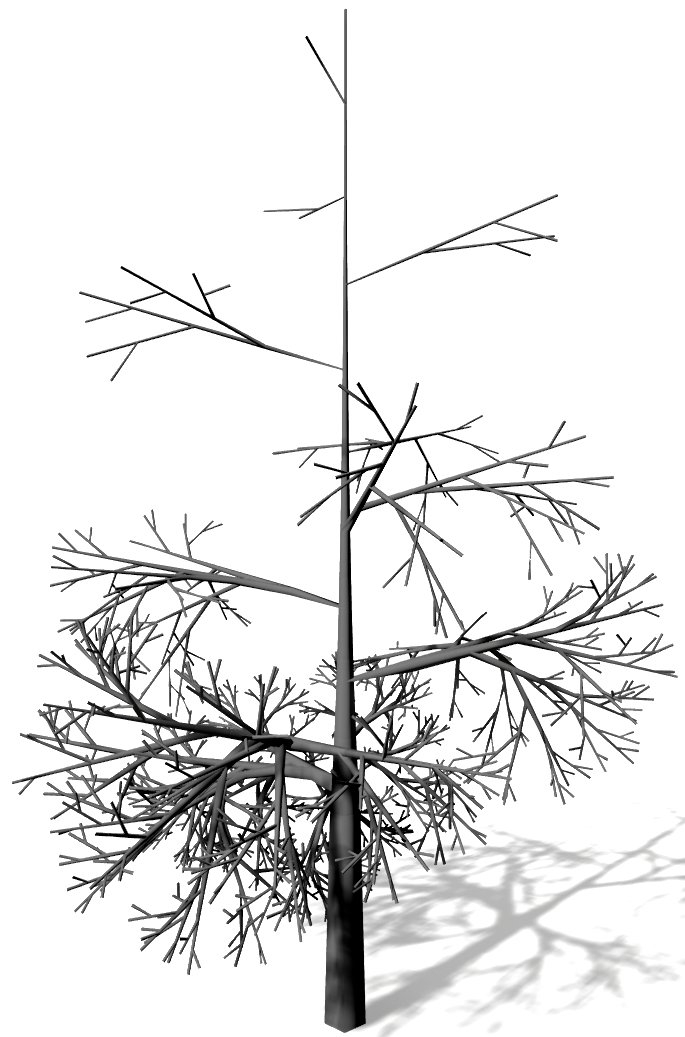
\includegraphics[height=.21\textheight]{images/LS_Monopodial_4.png}
		\caption{}
		\label{subfig:LS_Monopodial_4}
	\end{subfigure}
	\caption{Beispiele monopodialen Wachstums, entspricht der n-fachen Ableitung des Axioms anhand der Produktionsregeln aus Gleichung \ref{eq:ProdMonopodial}. Eigene Abbildungen.}
	\label{fig:LS_Monopodial}
\end{figure}

\subsection{Sympodiales Wachstum}
Beim sympodialen Wachstum bildet ein Ast mehrere Abzweigungen in einem Winkel ungleich $0\degree$. Der sich verzweigende Ast wächst daraufhin nicht weiter. \cite[S.14]{Deussen:05} \cite[S.58]{ABOP:04} Das folgende L-System simuliert ein solches Wachstum:

\begin{equation}
\begin{array}{llll}
\omega & : F(100)A(150) \\
p_1 & : A(l) &\rightarrow& F(l)\text{ }[\&(a1)\text{ }B(l*r1)]\text{ }/(180)\text{ }[\&(a2)\text{ }B(l*r2)] \\
p_2 &  : B(l) &\rightarrow& F(l)\text{ }[+(a1)\text{ }/(d1)\text{ }B(l*r1)]\text{ }[-(a2)\text{ }\backslash(d2)\text{ }B(l*r2)]
\end{array}
\label{eq:ProdSympodial}
\end{equation} 
\cite[S.59]{ABOP:04}
Die Produktionsregel $p_1$ beschreibt die Bildung der ersten, sich gegenüberliegenden, Abzweigungen während $p_2$ das Wachstum der abzweigenden Äste beschreibt, welche sich ebenfalls zu zwei Nebenästen aufteilen. $a_1$ und $a_2$ entsprechen den Abzweigungswinkeln, $r_1$ und $r_2$ den Wachstumsfaktoren pro Ableitung der Nebenäste. $d_1$ und $d_2$ beschreiben die Rotation eines Nebenastes um seine eigene Achse, bevor die nächste Abzweigung entsteht.

Abbildung \ref{fig:LS_Sympodial} zeigt Beispiele für sympodiale Baumstrukturen, Tabelle \ref{tab:LS_Sympodial} die verwendeten Konstantenwerte. Es findet kein Einfluss durch Tropismus statt.

\begin{center}
	\begin{tabulary}{\textwidth}{|C|C|C|C|C|C|C|C|}
		\hline 
		Abbildung & $n$ & $a_1$ & $a_2$ & $r_1$ & $r_2$ & $d_1$ & $d_2$ \\ 
		\hline 
		a & 10 & 5.0 & 65.0 & 0.9 & 0.75 & 50.0 & 50.0 \\ 
		\hline 
		b & 10 & 20.0 & 50.0 & 0.9 & 0.75 & 50.0 & 50.0 \\ 
		\hline 
		c & 10 & 35.0 & 35.0 & 1.0 & 0.8 & 50.0 & 50.0 \\ 
		\hline 
		d & 10 & 30.0 & 40.0 & 0.95 & 0.9 & 110.0 & 110.0 \\ 
		\hline 
	\end{tabulary} 
	\captionof{table}{Konstantenwerte der in Abbildung \ref{fig:LS_Sympodial} dargestellten sympodialen Baumstrukturen.} 
	\label{tab:LS_Sympodial}
\end{center}

\begin{figure} [hbtp]
	\centering
	\begin{subfigure}[t]{.45\textwidth}
		\centering
		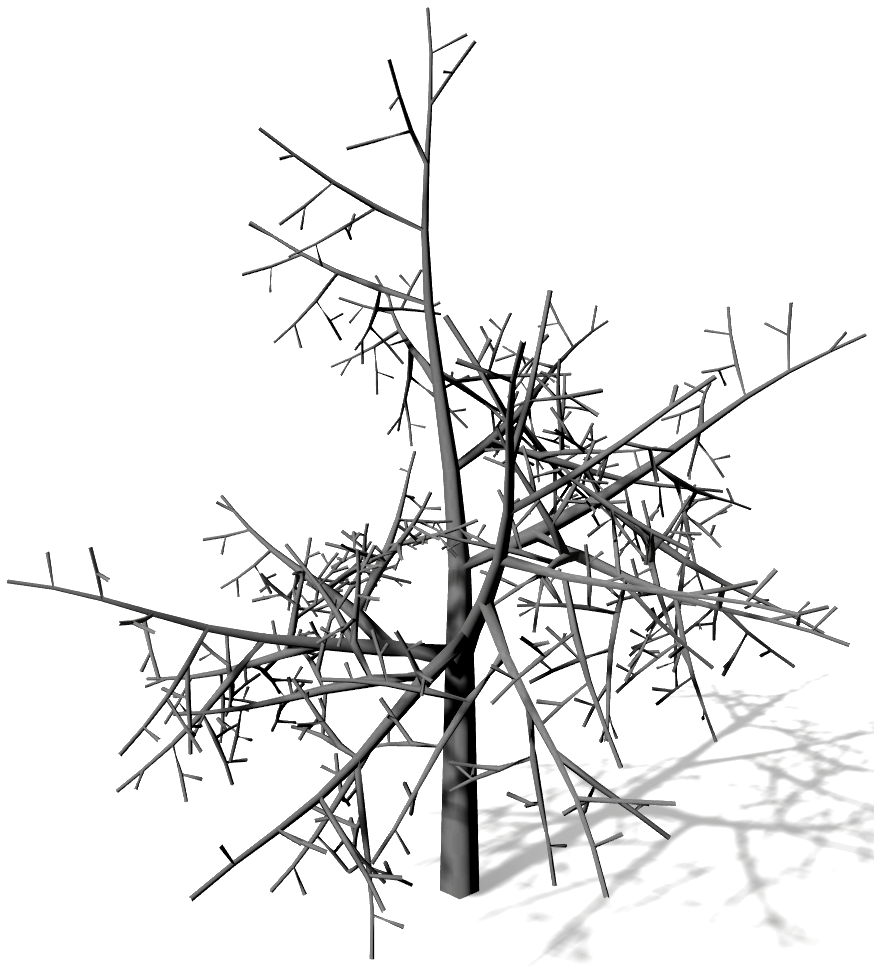
\includegraphics[height=.21\textheight]{images/LS_Sympodial_1.png}
		\caption{}
		\label{subfig:LS_Sympodial_1}
	\end{subfigure}
	\begin{subfigure}[t]{.45\textwidth}
		\centering
		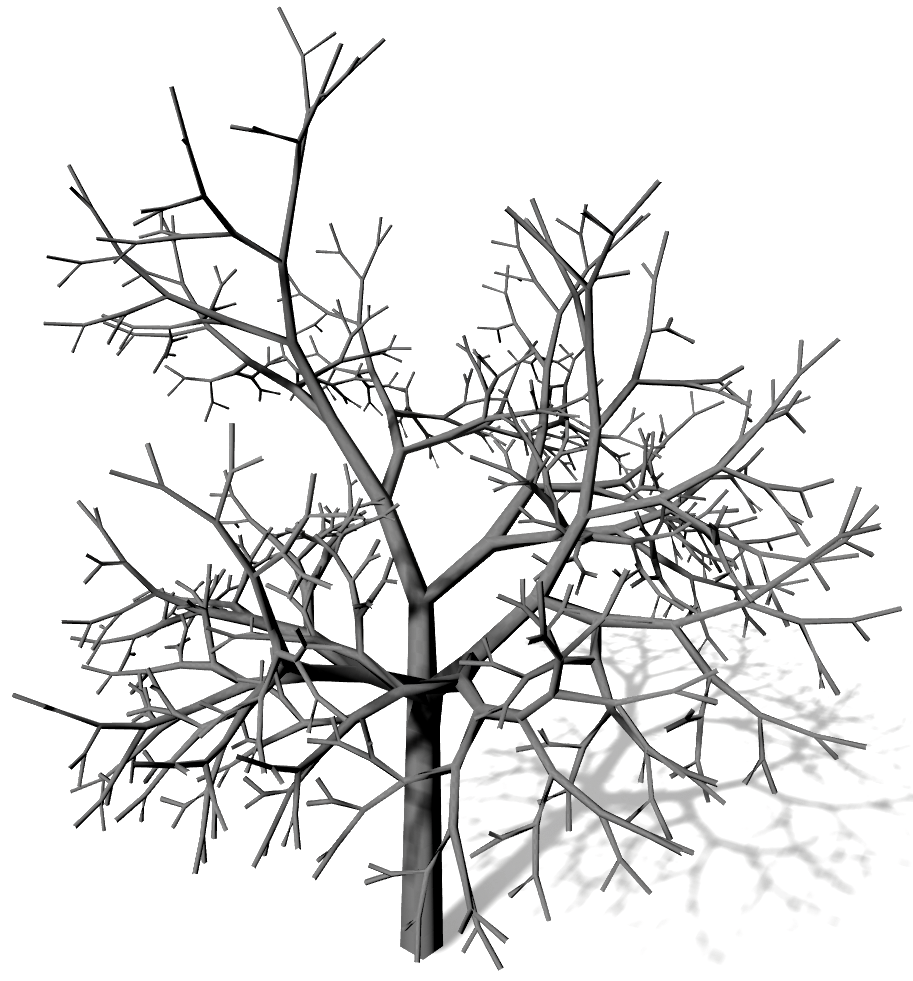
\includegraphics[height=.21\textheight]{images/LS_Sympodial_2.png}
		\caption{}
		\label{subfig:LS_Sympodial_2}
	\end{subfigure}	
	\begin{subfigure}[t]{.45\textwidth}
		\centering
		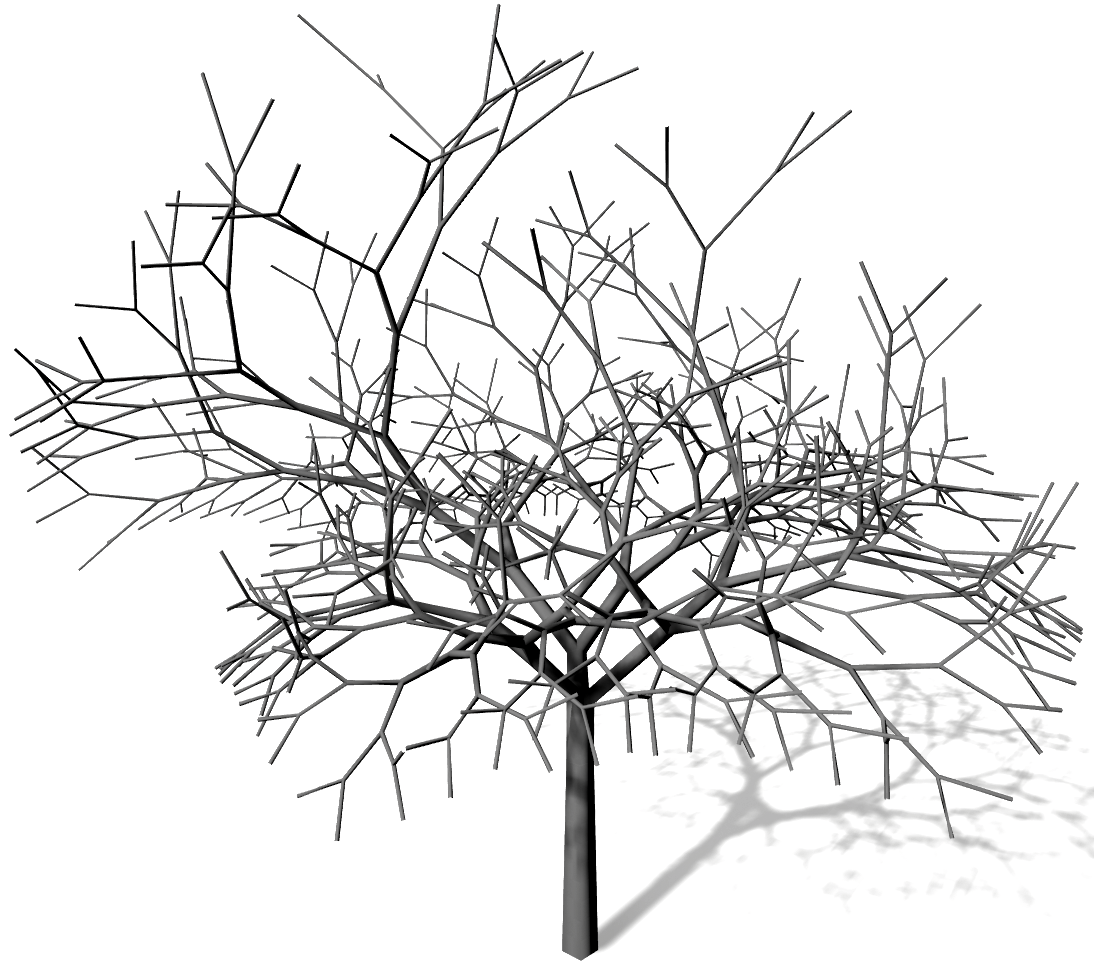
\includegraphics[height=.21\textheight]{images/LS_Sympodial_3.png}
		\caption{}
		\label{subfig:LS_Sympodial_3}
	\end{subfigure}
	\begin{subfigure}[t]{.45\textwidth}
		\centering
		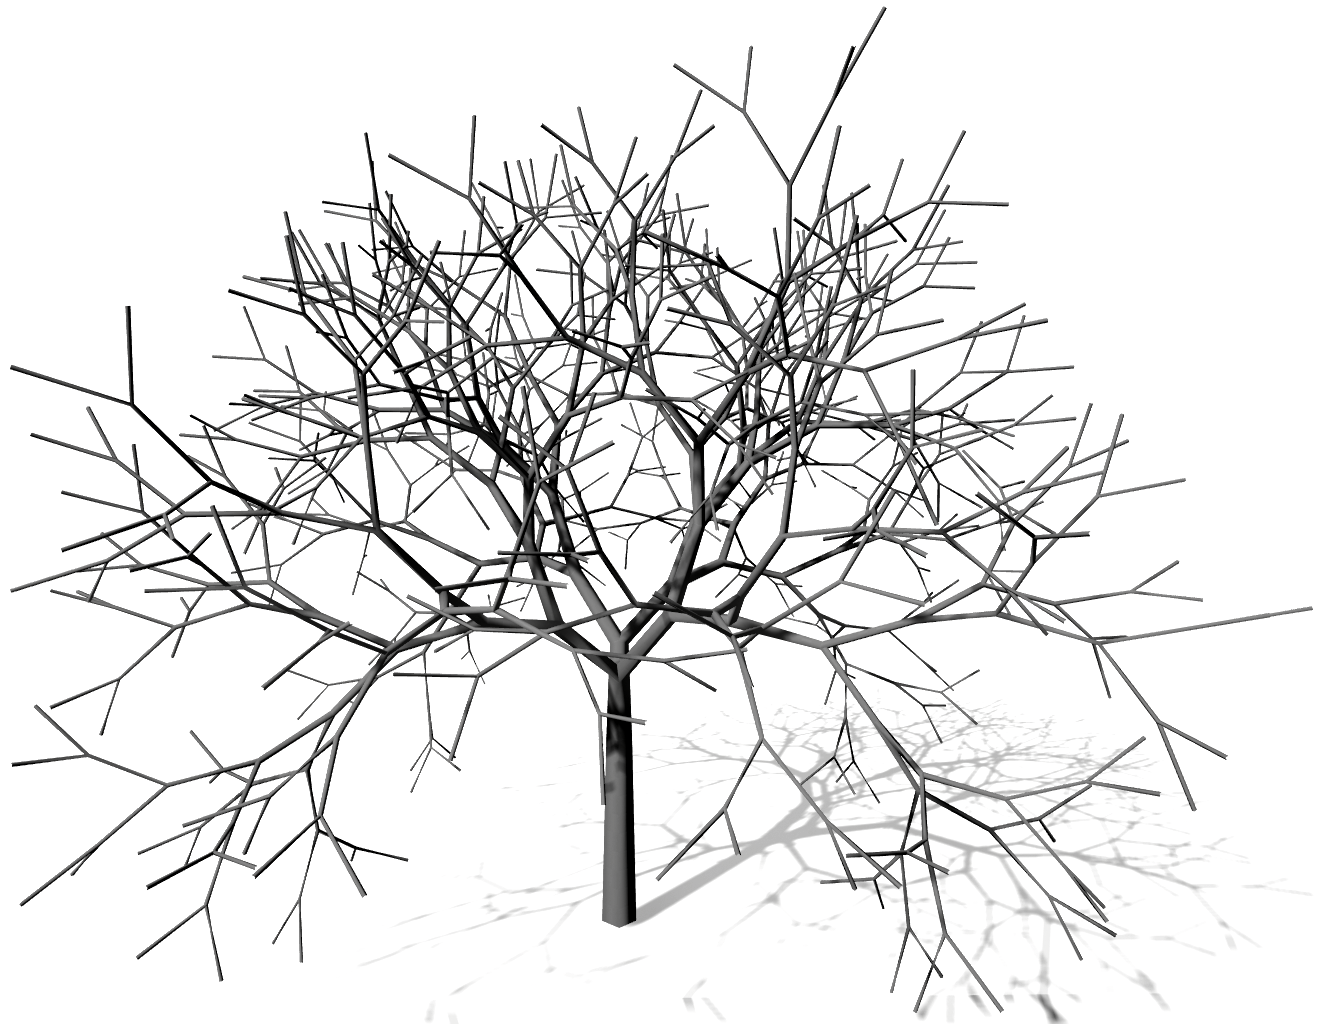
\includegraphics[height=.21\textheight]{images/LS_Sympodial_4.png}
		\caption{}
		\label{subfig:LS_Sympodial_4}
	\end{subfigure}
	\caption{Beispiele sympodialen Wachstums, entspricht der n-fachen Ableitung des Axioms anhand der Produktionsregeln aus Gleichung \ref{eq:ProdSympodial}. Eigene Abbildungen.}
	\label{fig:LS_Sympodial}
\end{figure}


\subsection{Ternäre Verzweigungen}

Eine andere Herangehensweise zur Bestimmung von L-Systemen für realistisch wirkende Baumstrukturen ist die Beschreibung von Selbstähnlichkeit, wie sie oft in der Natur zu finden ist. \cite[S.173]{ABOP:04} Das L-System aus Gleichung \ref{eq:ProdTernary} entspricht einem Wachstum, in welchem drei Abzweigungen mithilfe von Produktion $p_1$ auf dieselbe Art erstellt werden. In Produktion $p_2$ wird beschrieben wie Kanten aus vorhergehenden Ableitungen um einen Faktor $l_r$ verlängert werden. \cite[S.58]{ABOP:04}

\begin{equation}
\begin{array}{llll}
\omega & : /(45)A \\
p_1 & : A &\rightarrow& F(l_s)\text{ }[\&(a)\text{ }F(l_s)\text{ }A]\text{ }/(d1)\text{ }[\&(a)\text{ }F(l_s)\text{ }A]\text{ }/(d2)\text{ }[\&(a)\text{ }F(l_s)\text{ }A] \\
p_2 &  : F(l) &\rightarrow& F(l * l_r)
\end{array}
\label{eq:ProdTernary}
\end{equation} 
\cite[S.60]{ABOP:04}

$a$ entspricht dem Abzweigungswinkel von der Ursprungsachse, $d_1$ und $d_2$ der Rotation um die Achse, bevor eine neue Abzweigung produziert wird. $l_s$ ist die Anfangslänge der Kanten. \cite[S.58]{ABOP:04}

Abbildung \ref{fig:LS_Ternary} zeigt verschiedene ternär verzweigte Baumstrukturen, die auf den in Tabelle \ref{tab:LS_Ternary} gelisteten Konstantenwerten aufgebaut sind.

\begin{center}
	\begin{tabulary}{\textwidth}{|C|C|C|C|C|C|C|}
		\hline 
		Abbildung & $n$ & $a$ & $d_1$ & $d_2$ & $l_r$ & $l_s$ \\ 
		\hline 
		a & 6 & 19.0 & 95.0 & 132.0 & 1.1 & 50.0 \\ 
		\hline 
		b & 8 & 19.0 & 137.5 & 137.5 & 1.2 & 50.0 \\ 
		\hline 
		c & 8 & 27.0 & 77.0 & 77.0 & 1.3 & 50.0 \\ 
		\hline 
		d & 8 & 31.0 & 120.0 & 190.0 & 1.2 & 50.0 \\ 
		\hline 
	\end{tabulary} 
	\captionof{table}{Konstantenwerte der in Abbildung \ref{fig:LS_Ternary} dargestellten ternär verzweigten Baumstrukturen.} 
	\label{tab:LS_Ternary}
\end{center}

\begin{figure} [hbtp]
	\centering
	\begin{subfigure}[t]{.45\textwidth}
		\centering
		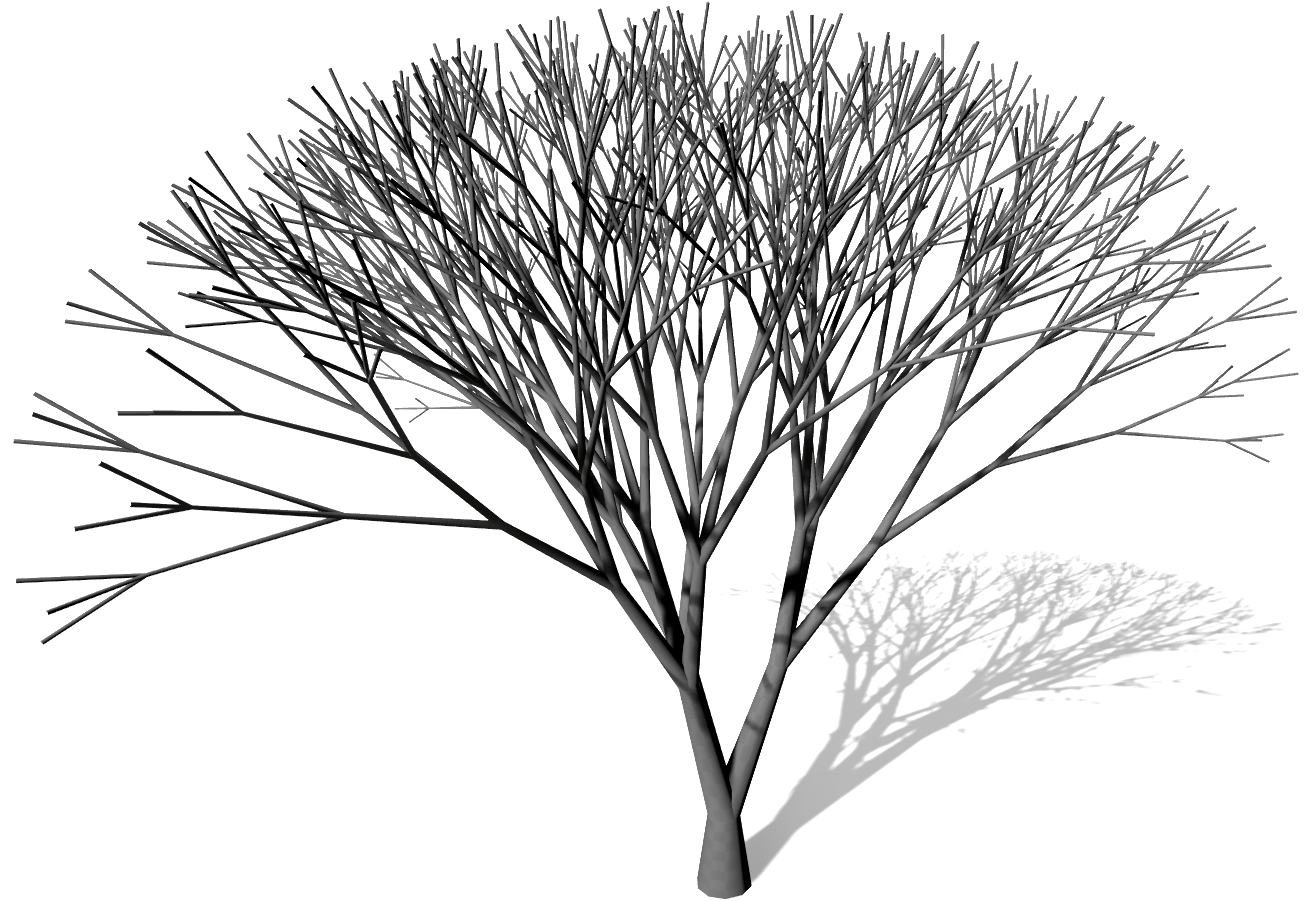
\includegraphics[width=\linewidth]{images/LS_Ternary_1.png}
		\caption{}
		\label{subfig:LS_Ternary_1}
	\end{subfigure}
	\begin{subfigure}[t]{.45\textwidth}
		\centering
		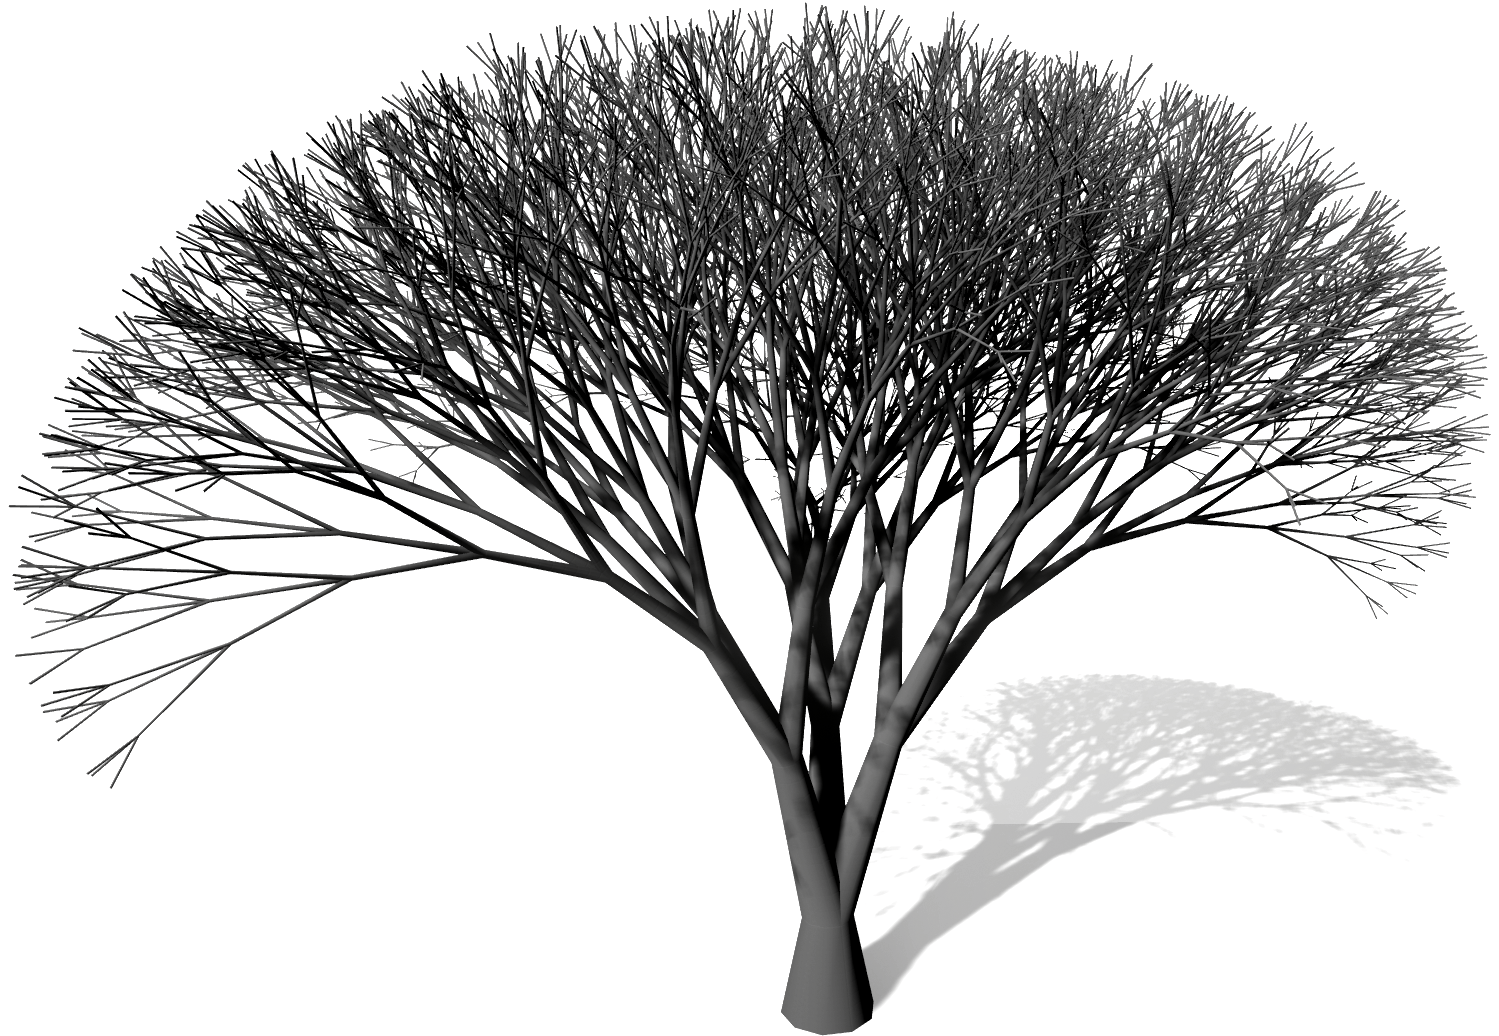
\includegraphics[width=\linewidth]{images/LS_Ternary_2.png}
		\caption{}
		\label{subfig:LS_Ternary_2}
	\end{subfigure}	
	\begin{subfigure}[t]{.45\textwidth}
		\centering
		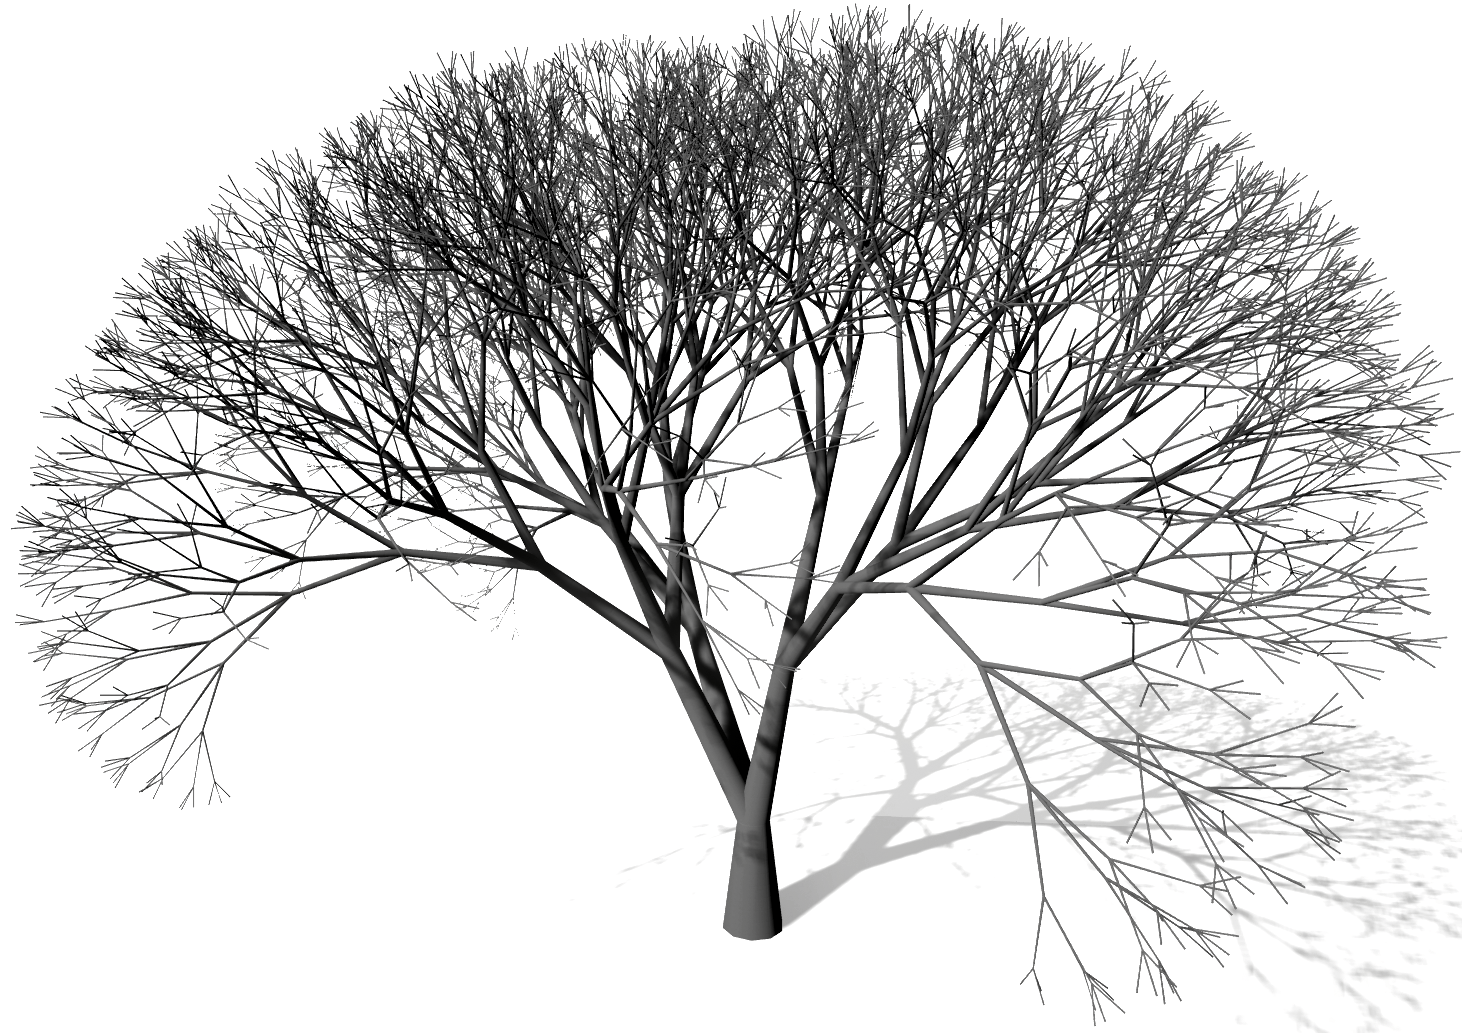
\includegraphics[width=\linewidth]{images/LS_Ternary_3.png}
		\caption{}
		\label{subfig:LS_Ternary_3}
	\end{subfigure}
	\begin{subfigure}[t]{.45\textwidth}
		\centering
		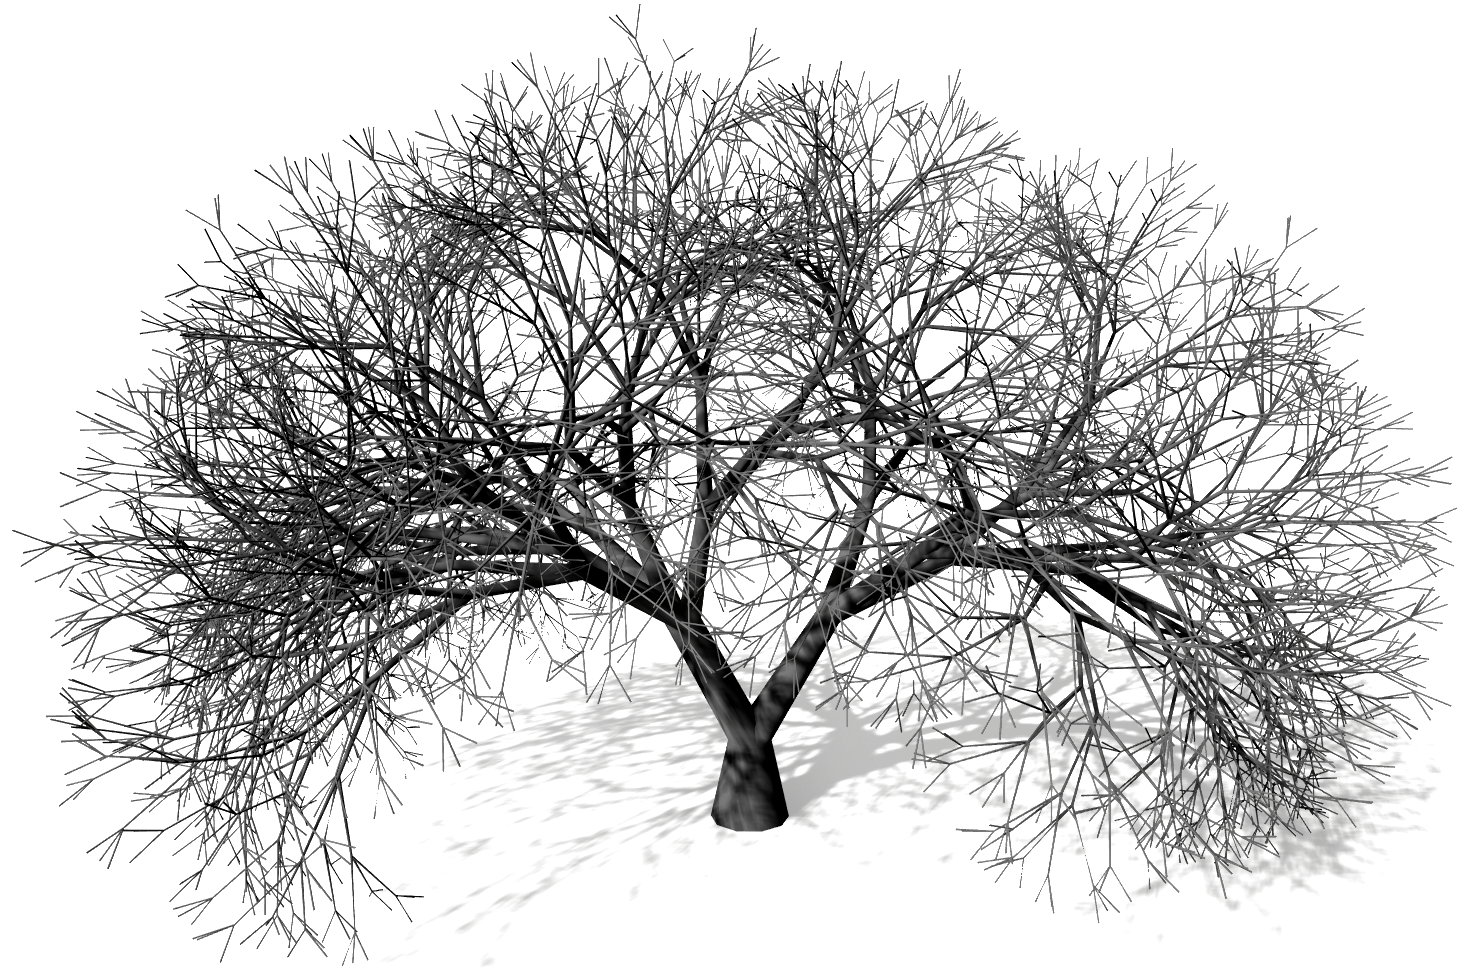
\includegraphics[width=\linewidth]{images/LS_Ternary_4.png}
		\caption{}
		\label{subfig:LS_Ternary_4}
	\end{subfigure}
	\caption{Beispiele ternären Wachstums, entspricht der n-fachen Ableitung des Axioms anhand der Produktionsregeln aus Gleichung \ref{eq:ProdTernary}. Eigene Abbildungen.}
	\label{fig:LS_Ternary}
\end{figure}


\subsection{Tropismus}

Der Einfluss von Tropismus führt, bei Eingabe derselben Werte bei den restlichen Parametern, zu visuell unterschiedlichen Ergebnissen. Dadurch können reale Einflüsse wie die Einwirkung von Wind, Sonne und Gravitation simuliert sowie die Wiederverwendbarkeit von L-System Definitionen erhöht werden. \cite[S.58]{ABOP:04}

Abbildung \ref{fig:LS_Ternary_Tropism} zeigt den Einfluss von Tropismus auf Baumstrukturen aus Abbildung \ref{fig:LS_Ternary}, welche ohne die Einwirkung von Tropismus produziert wurden.


\begin{figure} [hbtp]
	\centering
	\begin{subfigure}[t]{.45\textwidth}
		\centering
		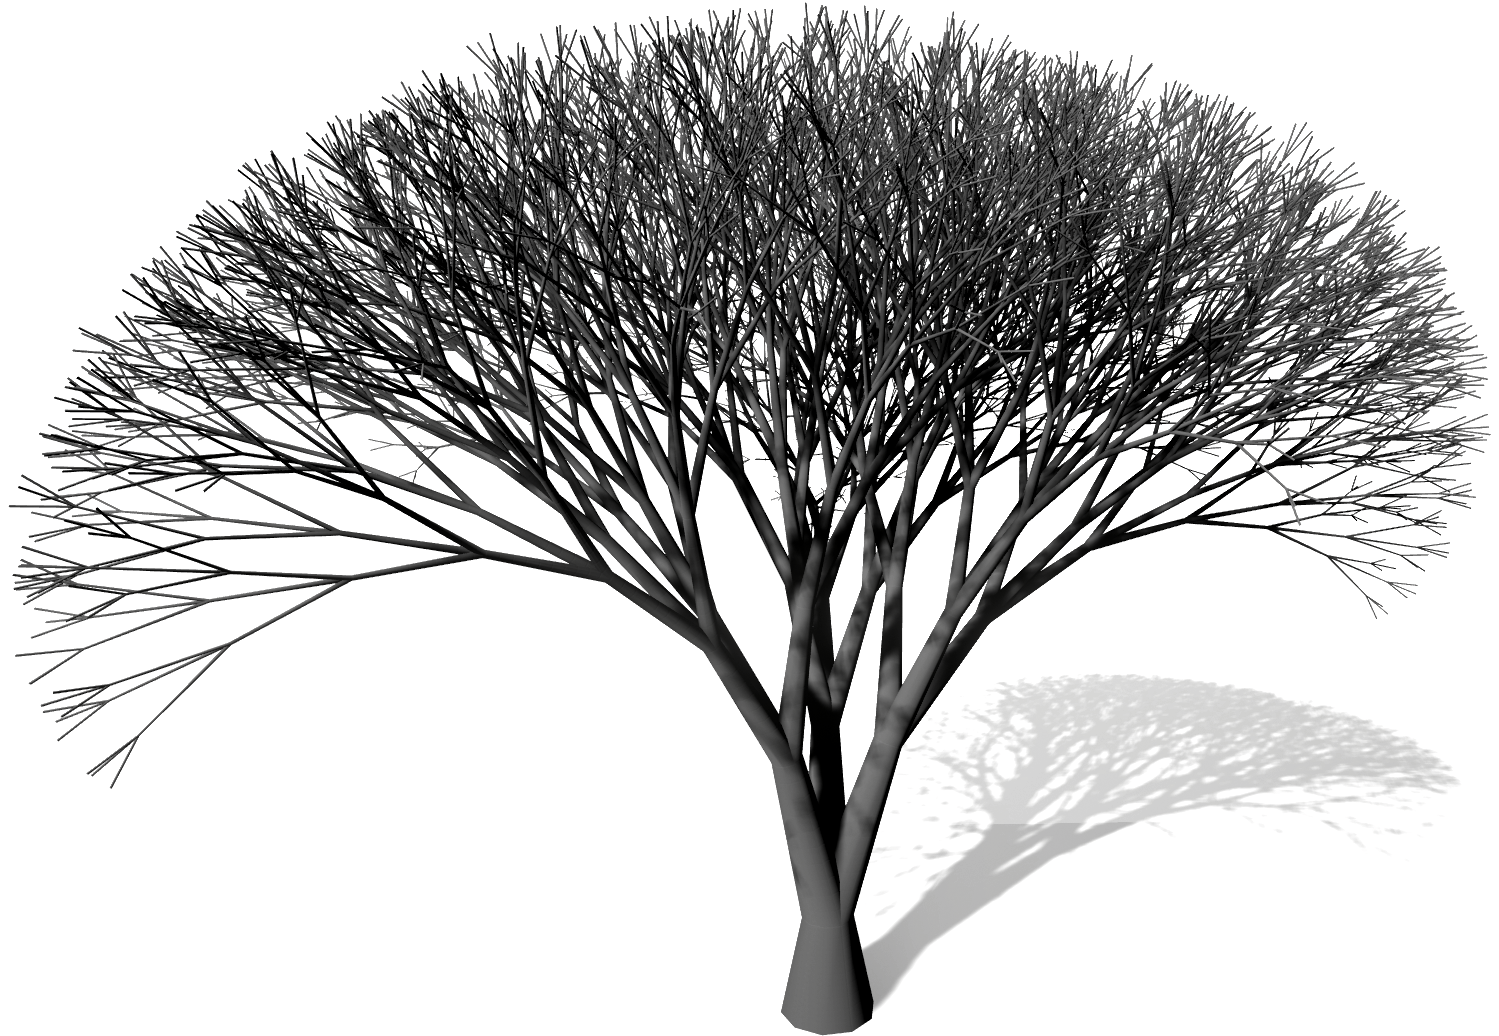
\includegraphics[width=\linewidth]{images/LS_Ternary_2.png}
		\caption{$\overrightarrow{T} = \overrightarrow{0}$, $e = 0$ \\ Entspricht Abbildung \ref{subfig:LS_Ternary_2}.}
		\label{subfig:LS_Ternary_2.2}
	\end{subfigure}
	\begin{subfigure}[t]{.45\textwidth}
		\centering
		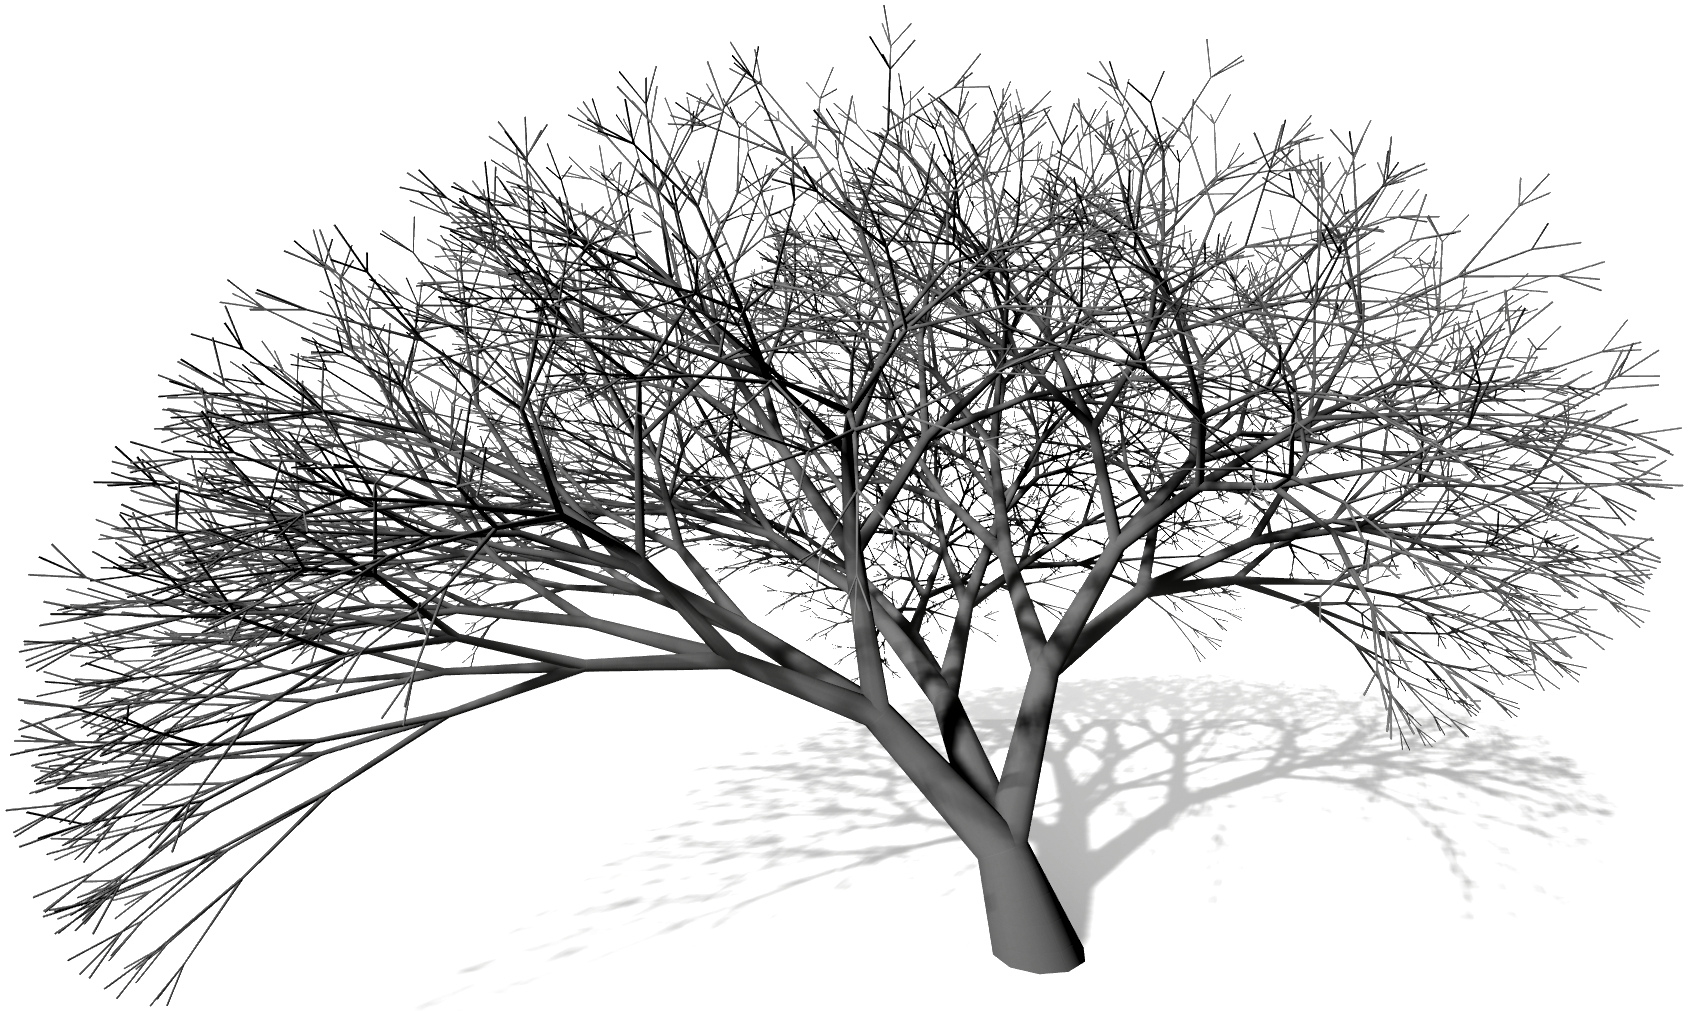
\includegraphics[width=\linewidth]{images/LS_Ternary_2_Tropism.png}
		\caption{$\overrightarrow{T} = \protect\begin{pmatrix}
			0 \\
			-0.5 \\
			-1
			\protect\end{pmatrix}$, $e = 0.5$}
		\label{subfig:LS_Ternary_2_Tropism}
	\end{subfigure}	
	\begin{subfigure}[t]{.45\textwidth}
		\centering
		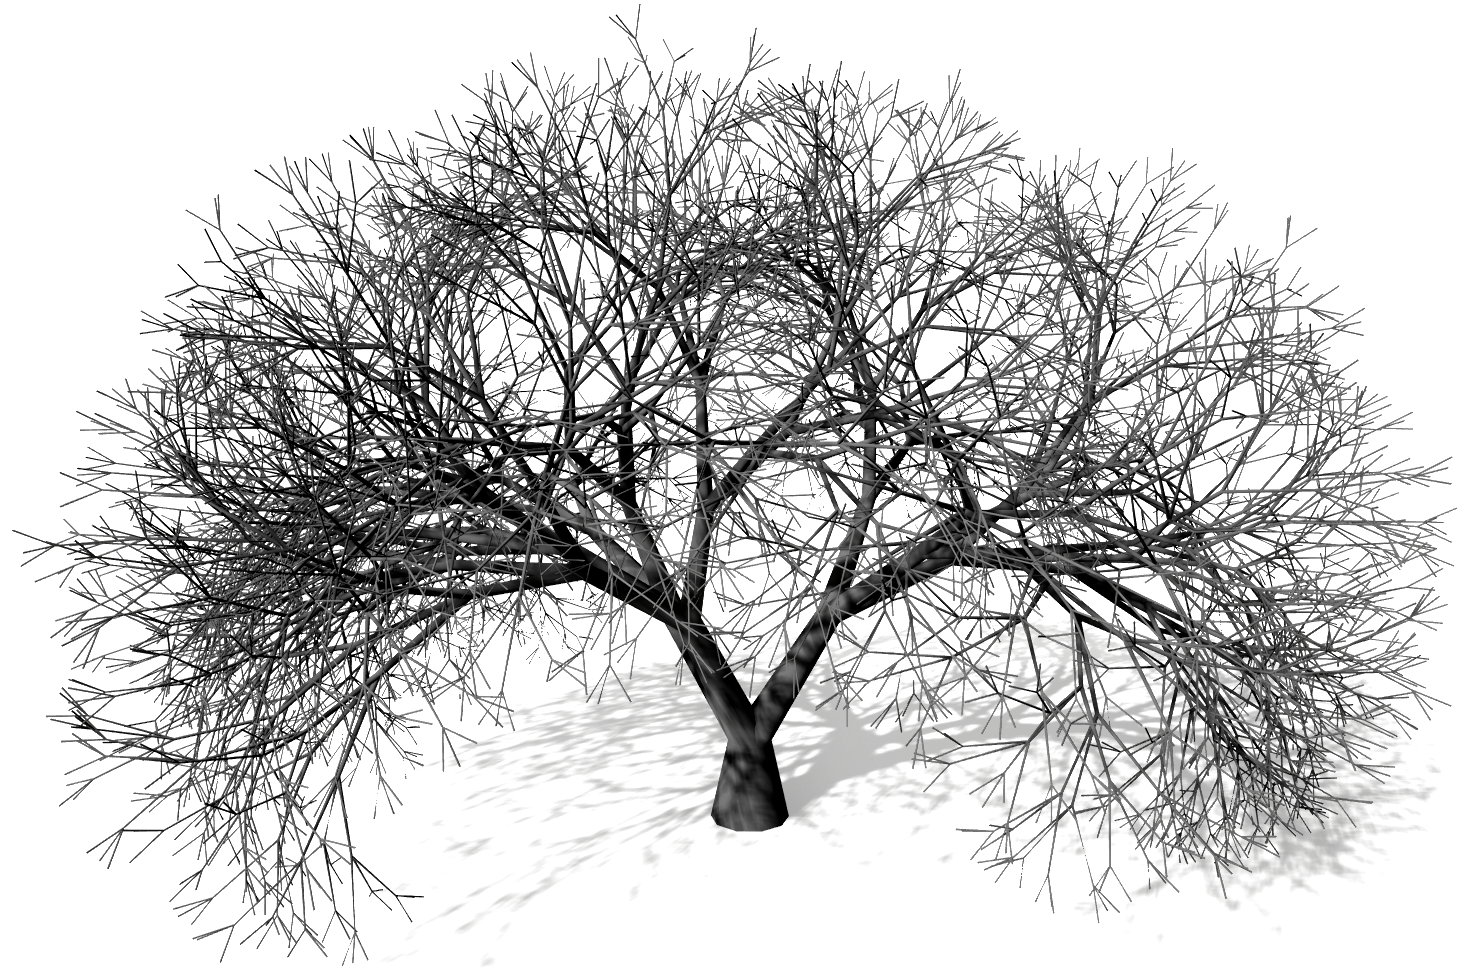
\includegraphics[width=\linewidth]{images/LS_Ternary_4.png}
		\caption{$\overrightarrow{T} = \overrightarrow{0}$, $e = 0$\\ Entspricht Abbildung \ref{subfig:LS_Ternary_4}.}
		\label{subfig:LS_Ternary_4.2}
	\end{subfigure}
	\begin{subfigure}[t]{.45\textwidth}
		\centering
		\includegraphics[width=\linewidth]{images/LS_Ternary_4_Tropism.png}
		\caption{$\overrightarrow{T} = \protect\begin{pmatrix}
			1 \\
			0 \\
			1
			\protect\end{pmatrix}$, $e = 0.3$}
		\label{subfig:LS_Ternary_4_Tropism}
	\end{subfigure}
	\caption{Beispiele ternären Wachstums mit und ohne Einfluss durch Tropismus. Entspricht der n-fachen Ableitung des Axioms anhand der Produktionsregeln aus Gleichung \ref{eq:ProdTernary}. Die linken und rechten Abbildungen unterscheiden sich jeweils im Tropismusvektor $\protect\overrightarrow{T}$ und im Biegsamkeitsfaktor $e$. Eigene Abbildungen.}
	\label{fig:LS_Ternary_Tropism}
\end{figure}

\section{Space-Colonization-Actor}

Die Space-Colonization Implementierung ermöglicht es durch die Angabe einiger weniger Parameter eine Vielzahl verschiedener Baumstrukturen zu generieren. \cite[S.3]{SpaceColonizationAlgorithm:07} Im Folgenden wird der Einfluss dieser Parameter auf die Ergebnisse untersucht. Es werden jeweils sich unterscheidende Parameterwerte angegeben.

\subsection{Einflussbereiche}

Die Verteilung und Anzahl der Einflusspunkte hat starke Auswirkungen auf die sich ergebende Baumstruktur. Je weniger Einflusspunkte existieren, desto größer ist die Wirkung jedes Punktes auf die Position der neuen Knotenpunkte und resultiert in einer spärlich bewachsenen Baumkrone mit kantigen, ungleichmäßig verteilten Ästen. Wird die Anzahl der Einflusspunkte erhöht, entsteht eine dicht bewachsene Baumkrone mit leicht kurvenförmigen, gleichmäßig verteilten Ästen. \cite[S.3]{SpaceColonizationAlgorithm:07}

Weiterhin passt sich die generierte Baumstruktur dem Bereich an, in welchem die Einflusspunkte generiert werden. Es können entweder einzelne Bereichprimitive, wie eine Kugel- oder Zylinderform, oder mehrere miteinander verknüpfte Einflussbereiche verwendet werden. \cite[S.4]{SpaceColonizationAlgorithm:07}

\begin{figure} [hbtp]
	\centering
	\begin{subfigure}[t]{.45\textwidth}
		\centering
		\includegraphics[height=.21\textheight]{images/SCA_Einfluss_Sphere_Low.png}
		\caption{Kugelförmig mit Radius $r = 500$, $N = 1000$}
		\label{subfig:SCA_Einfluss_Sphere_Low}
	\end{subfigure}
	\hspace{.05\linewidth}
	\begin{subfigure}[t]{.45\textwidth}
		\centering
		\includegraphics[height=.21\textheight]{images/SCA_Einfluss_Sphere_High.png}
		\caption{Kugelförmig mit Radius $r = 500$, $N = 10000$}
		\label{subfig:SCA_Einfluss_Sphere_High}
	\end{subfigure}	
	\begin{subfigure}[t]{.45\textwidth}
		\centering
		\includegraphics[height=.21\textheight]{images/SCA_Einfluss_Cylinder_Low.png}
		\caption{Zylinderförmig mit Höhe $h=1000$ und Radius $r_z = 300$, $N = 1000$}
		\label{subfig:SCA_Einfluss_Cylinder_Low}
	\end{subfigure}
	\hspace{.05\linewidth}
	\begin{subfigure}[t]{.45\textwidth}
		\centering
		\includegraphics[height=.21\textheight]{images/SCA_Einfluss_Cylinder_High.png}
		\caption{Zylinderförmig mit Höhe $h=1000$ und Radius $r_z = 300$, $N = 10000$}
		\label{subfig:SCA_Einfluss_Cylinder_High}
	\end{subfigure}
	\caption{Wirkung der Anzahl der Einflusspunkte $n$ und der Form des Einflussbereichs auf die generierte Baumstruktur. Eigene Abbildungen.}
	\label{fig:SCA_Einfluss}
\end{figure}
 
 \begin{figure} [hbtp]
 	\centering
 	\begin{subfigure}[t]{.45\textwidth}
 		\centering
 		\includegraphics[height=.21\textheight]{images/SCA_MultipleSpheres_Points.png}
 		\caption{Punktewolke.}
 		\label{subfig:SCA_MultipleSpheres_Points}
 	\end{subfigure}
 	\hspace{.05\linewidth}
 	\begin{subfigure}[t]{.45\textwidth}
 		\centering
 		\includegraphics[height=.21\textheight]{images/SCA_MultipleSpheres_Grown.png}
 		\caption{Resultierende Baumstruktur.}
 		\label{subfig:SCA_MultipleSpheres_Grown}
 	\end{subfigure}	
 	\caption{Verbindung von drei kugelförmigen Einflussbereichen zu einem Bereich. Die Kugeln haben jeweils den Radius $r=500$ und $N=2000$. Eigene Abbildungen.}
 	\label{fig:SCA_MultipleSpheres}
 \end{figure}
 
\subsection{Wachstumsparameter}

Bei den Parametern, welche sich direkt auf die Positionierung neuer Knoten auswirken, handelt es sich um Minimalradius, Einflussradius, Schrittweite, Tropismus, Maximale Zweigtiefe, gewichtetes Wachstum, den maximalen Grad eines Knotens und die maximale Anzahl von durchgeführten Iterationen.

\paragraph{Minimalradius und Einflussradius}

Der Minimalradius $d_k$ hat eine ähnliche Wirkung auf eine generierte Baumstruktur wie die Anzahl der Einflusspunkte $N$. Je höher der Minimalradius $d_k$, desto weniger Abzweigungen werden gebildet, da nach der Bildung eines neuen Astsegments Einflusspunkte entfernt werden, die zuvor eine solche Abzweigung bewirkt hätten. Die Baumkrone erscheint spärlicher bewachsen, die entstandenen Äste sind jedoch kurvenreicher, da auf die wenigen wachsenden Äste mehr Einflusspunkte einwirken -- das Entfernen oder Hinzufügen einzelner Einflusspunkte hat somit nur eine kleine Auswirkung auf die Position eines in der nächsten Iteration neu hinzugefügten Astsegments. \cite[S.3]{SpaceColonizationAlgorithm:07}

Je kleiner der Einflussradius $d_i$, desto knorriger wirkt ein Baum, da Astsegmente in jedem Iterationsschritt in den Wirkungsbereich eines Einflusspunktes geraten und im nächsten Schritt wieder verlassen. \cite[S.4]{SpaceColonizationAlgorithm:07}

Abbildung \ref{fig:SCA_KDRI} zeigt Beispiele der Wirkung unterschiedlicher Werte für Einflussradius und Minimalradius.

\begin{figure} [hbtp]
	\centering
	\begin{subfigure}[t]{.45\textwidth}
		\centering
		\includegraphics[height=.21\textheight]{images/SCA_KDRI_LowKD_LowRI.png}
		\caption{$d_k = 80$, $d_i = 150$}
		\label{subfig:SCA_KDRI_LowKD_LowRI}
	\end{subfigure}
	\hspace{.05\linewidth}
	\begin{subfigure}[t]{.45\textwidth}
		\centering
		\includegraphics[height=.21\textheight]{images/SCA_KDRI_HighKD_LowRI.png}
		\caption{$d_k = 130$, $d_i = 150$}
		\label{subfig:SCA_KDRI_HighKD_LowRI}
	\end{subfigure}	
	\begin{subfigure}[t]{.45\textwidth}
		\centering
		\includegraphics[height=.21\textheight]{images/SCA_KDRI_LowKD_HighRI.png}
		\caption{$d_k = 80$, $d_i = 1000$}
		\label{subfig:SCA_KDRI_LowKD_HighRI}
	\end{subfigure}
	\hspace{.05\linewidth}
	\begin{subfigure}[t]{.45\textwidth}
		\centering
		\includegraphics[height=.21\textheight]{images/SCA_KDRI_HighKD_HighRI.png}
		\caption{$d_k = 130$, $d_i = 1000$}
		\label{subfig:SCA_KDRI_HighKD_HighRI}
	\end{subfigure}
	\caption{Wirkung von Einflussradius $d_i$ und Minimalradius $d_k$ auf die generierte Baumstruktur. Es wurde die Schrittweite $D = 10$ verwendet. Eigene Abbildungen.}
	\label{fig:SCA_KDRI}
\end{figure}

\paragraph{Tropismus, maximale Zweigtiefe, maximaler Grad und gewichtetes Wachstum}

Ebenso wie bei der Implementierung von L-Systemen kann der Einfluss eines Tropismusvektors $\overrightarrow{T}$ das Wachstumsverhalten der Space-Colonization Implementierung bei gleichen Parameterwerten stark in eine bestimmte Richtung beeinflussen. Werte auf der horizontalen Ebene erwecken den Anschein von Einwirkung durch Wind. Positive Werte auf der Z-Achse entsprechen dem Streben einer Pflanze der Sonnenposition entgegen zu wachsen, negative Werte auf der Z-Achse simulieren die Einwirkung auf das Wachstum durch Gravitation. \cite[S.5]{SpaceColonizationAlgorithm:07}

Die maximale Zweigtiefe $max_Z$ begrenzt die Anzahl der Abzweigungen, die von dem Wurzel-Astsegment ausgehend zu jedem Astsegment ohne Nachfolger gebildet werden können. Bei niedrigen Werten führt dies zur Bildung weniger, kurvenförmiger Astsegmente.

Der maximale Grad $max_{grad}$ begrenzt die Anzahl der Abzweigungen, die von einem einzelnen Astsegment ausgehen können. Da Astsegmente nur in sehr dichten Baumstrukturen -- Strukturen mit vielen Einflusspunkten und einem niedrigen Minimalradius -- mehr als zwei Nachfolger bilden, hat dieser Parameter eine eingeschränkte visuelle Einwirkung. In dichten Baumstrukturen ermöglicht er es jedoch, bei minimaler visueller Einwirkung, die Anzahl der erstellten Vertizes zu begrenzen. Die Wahl von $max_{grad} = 1$ sorgt für die Bildung eines durchgängigen, in sich verdrehten Astes ohne Abzweigungen.

In Abbildung \ref{fig:SCA_Sonst} werden Beispiele für die Wirkung der beschriebenen Parameter gezeigt.

\begin{figure} [hbtp]
	\centering
	\begin{subfigure}[t]{.45\textwidth}
		\centering
		\includegraphics[height=.21\textheight]{images/SCA_Sonst_Ursprung.png}
		\caption{$d_k = 60$, $d_i = 150$, $\protect\overrightarrow{T} = (0,0,0.2)$, $r = 600$, $N = 2000$, $max_Z = 20$, $max_{grad} = 20$, kein gewichtetes Wachstum.}
		\label{subfig:SCA_Sonst_Ursprung}
	\end{subfigure}
	\hspace{.05\linewidth}
	\begin{subfigure}[t]{.45\textwidth}
		\centering
		\includegraphics[height=.21\textheight]{images/SCA_Sonst_Tropism_Wind.png}
		\caption{$\protect\overrightarrow{T} = (0,0.8,0)$}
		\label{subfig:SCA_Sonst_Tropism_Wind}
	\end{subfigure}	
	\begin{subfigure}[t]{.45\textwidth}
		\centering
		\includegraphics[height=.21\textheight]{images/SCA_Sonst_Tropism_Grav.png}
		\caption{$\protect\overrightarrow{T} = (0,0,-0.8)$}
		\label{subfig:SCA_Sonst_Tropism_Grav}
	\end{subfigure}
	\hspace{.05\linewidth}
	\begin{subfigure}[t]{.45\textwidth}
		\centering
		\includegraphics[height=.21\textheight]{images/SCA_Sonst_Zweigtiefe.png}
		\caption{$max_Z = 2$}
		\label{subfig:SCA_Sonst_Zweigtiefe}
	\end{subfigure}
	\begin{subfigure}[t]{.45\textwidth}
		\centering
		\includegraphics[height=.21\textheight]{images/SCA_Sonst_Grad.png}
		\caption{$max_{grad} = 1$}
		\label{subfig:SCA_Sonst_Grad}
	\end{subfigure}
	\begin{subfigure}[t]{.45\textwidth}
		\centering
		\includegraphics[height=.21\textheight]{images/SCA_Sonst_Grad2.png}
		\caption{$max_{grad} = 2$}
		\label{subfig:SCA_Sonst_Grad}
	\end{subfigure}
	\caption{Wirkung von Tropismus $\protect\overrightarrow{T}$, maximaler Zweigtiefe $max_Z$ und maximalem Knotengrad $max_{grad}$ auf die generierte Baumstruktur. Falls nicht weiter angegeben, wurden die in Abbildung \ref{subfig:SCA_Sonst_Ursprung} angegebenen Parameterwerte verwendet. Eigene Abbildungen.}
	\label{fig:SCA_Sonst}
\end{figure}
 
\paragraph{Schrittweite und maximale Anzahl durchzuführender Iterationen}

Je höher die Schrittweite $D$, desto knorriger wirkt ein Baum -- ähnlich dem Einflussradius -- da ein Astsegment in jedem Schritt Einflussradien betritt und verlässt oder ein neues Astsegment auf der gegenüberliegenden Seite eines Einflusspunktes gebildet wird und von diesem nun aus der entgegengesetzten Richtung beeinflusst wird. Weiterhin besitzen die Äste scharfe Kanten, da aufgrund der größeren Schrittweite weniger Vertizes generiert werden. Die Wahl einer niedrigen Schrittweite führt zur Bildung von Ästen mit leichten Kurven.

Die maximale Anzahl durchzuführender Iterationen $N_I$ beschränkt die Zahl von Space-Colonization Iterationen, die durchgeführt werden sollen. Die bisher gezeigten Beispiele wurden mit $N_I = 400$ durchgeführt und vor Erreichen dieser Zahl abgebrochen. Bei Festlegung niedrigerer Zahlen kann das Wachstum des Baumes beschränkt oder das Wachstumsverhalten im Laufe der Iterationen beobachtet werden.

Abbildung \ref{fig:SCA_SI} zeigt die Auswirkungen verschiedener Werte für die Schrittweite und die maximale Anzahl durchzuführender Iterationen bei gleichbleibender Verteilung der Einflusspunkte.

\begin{figure} [hbtp]
	\centering
	\begin{subfigure}[t]{.45\textwidth}
		\centering
		\includegraphics[height=.21\textheight]{images/SCA_SI_SchrittweiteHigh.png}
		\caption{$d_k = 100$, $d_i = 150$, $D = 50$, $N_I = 400$}
		\label{subfig:SCA_SI_SchrittweiteHigh}
	\end{subfigure}
	\hspace{.01\linewidth}
	\begin{subfigure}[t]{.45\textwidth}
		\centering
		\includegraphics[height=.21\textheight]{images/SCA_SI_SchrittweiteLow.png}
		\caption{$D = 5$}
		\label{subfig:SCA_SI_SchrittweiteLow}
	\end{subfigure}	
	\begin{subfigure}[t]{.2\textwidth}
		\centering
		\includegraphics[height=.11\textheight]{images/SCA_SI_Iterationen10.png}
		\caption{$D = 20$, $N_I = 10$}
		\label{subfig:SCA_SI_Iterationen10}
	\end{subfigure}
	\begin{subfigure}[t]{.2\textwidth}
		\centering
		\includegraphics[height=.11\textheight]{images/SCA_SI_Iterationen20.png}
		\caption{$N_I = 20$}
		\label{subfig:SCA_SI_Iterationen20}
	\end{subfigure}
	\begin{subfigure}[t]{.2\textwidth}
		\centering
		\includegraphics[height=.21\textheight]{images/SCA_SI_Iterationen40.png}
		\caption{$N_I = 40$}
		\label{subfig:SCA_SI_Iterationen40}
	\end{subfigure}
	\begin{subfigure}[t]{.35\textwidth}
		\centering
		\includegraphics[height=.21\textheight]{images/SCA_SI_Iterationen80.png}
		\caption{$N_I = 80$}
		\label{subfig:SCA_SI_Iterationen80}
	\end{subfigure}
	\caption{Wirkung von Schrittweite $D$ und maximaler Anzahl von Iterationen $N_I$ auf die generierte Baumstruktur. Eigene Abbildungen.}
	\label{fig:SCA_SI}
\end{figure}


\paragraph{Gewichtetes Wachstum}

Gewichtetes Wachstum erhöht die Wachstums-Schrittweite der Astsegmente in Abhängigkeit von der Zweigtiefe. Dies führt zu der erkennbaren Bildung eines Stammes und den davon abzweigenden Hauptästen. 

Die Einstellung erzielt den besten visuellen Eindruck in bestimmten Situationen: Bei Anwendung des Algorithmus auf große Werte für den Radius des Einflussbereichs $r$, der Anzahl von Einflusspunkten $N$, dem Einflussradius $d_i$ und bei einer Begrenzung des maximalen Anzahl durchzuführender Iterationen $N_I$, sodass die Baumstruktur nur einen Teil des Einflussbereichs ausfüllen kann. Dies erweckt den Anschein eines Baumes, dessen Wachstum noch nicht beendet ist.

Abbildung \ref{fig:SCA_GewWachstum} zeigt ein Beispiel für die Anwendung von gewichtetem Wachstum in der beschriebenen Situation.

\begin{figure} [hbtp]
	\centering
	\begin{subfigure}[t]{.45\textwidth}
		\centering
		\includegraphics[height=.3\textheight]{images/SCA_GewWachstum_Off.png}
		\caption{$N = 5000$, $r = 1000$, $N_I = 50$, $d_k = 50$, $d_i = 1000$, $D = 15$, $\protect\overrightarrow{T} = (0,0,0.7)$, kein gewichtetes Wachstum.}
		\label{subfig:SCA_GewWachstum_Off}
	\end{subfigure}
	\hspace{.05\linewidth}
	\begin{subfigure}[t]{.45\textwidth}
		\centering
		\includegraphics[height=.3\textheight]{images/SCA_GewWachstum_On.png}
		\caption{Mit gewichtetem Wachstum.}
		\label{subfig:SCA_GewWachstum_On}
	\end{subfigure}	
	\caption{Wirkung von gewichtetem Wachstum auf die generierte Baumstruktur. Eigene Abbildungen.}
	\label{fig:SCA_GewWachstum}
\end{figure}


\section{Effizienz}

Die Effizienz einer Software ist ihre Fähigkeit, mit den durch das Betriebssystem bereitgestellten Ressourcen ein bestimmtes Leistungsniveau zu erzielen. \cite[S.259]{Softwaremanagement:98} In Hinsicht auf prozedurale Generierung muss auf zwei wesentliche Punkte geachtet werden: Die Generierungszeit und das Laufzeitverhalten.

\subsection{Generierungszeit}

Die Zeit welche benötigt wird um eine Baumstruktur aufzubauen wird als Generierungszeit bezeichnet und wird bei den Implementierungen durch die vorgestellten Parameter beeinflusst. Mithilfe des Unreal Engine Profilers wurde die Ausführungszeit bestimmter Funktionen oder Funktionsabschnitte gemessen um die Abhängigkeiten zwischen Parametern und Generierungszeit zu bestimmen. \cite{Profiling:15}

\paragraph{L-System-Actor}

Die Generierungszeit der L-System Implementierung hängt linear von den durch die Turtle-Interpretation ausgeführten Bewegungen und Rotationen ab und macht diese somit abhängig von der Anzahl der Ableitungen sowie den angegebenen Produktionsregeln. Je öfter ein Axiom abgeleitet wird und je mehr Rotations- und Bewegungsaktionen in den Nachfolgern der Produktionsregeln angegeben sind, desto mehr Aktionen enthält die zu interpretierende Zeichenkette. 

\paragraph{Space-Colonization-Actor}

Die Generierungszeit der Space-Colonization Implementierung wird durch eine Vielzahl von Parametern festgelegt, welche die Anzahl der Einflusspunkte, wachsenden Astsegmente und durchzuführenden Iterationen beeinflussen. In einer Iteration wird jeder Einflusspunkt daraufhin überprüft, ob sich mindestens einer der wachsenden Astsegmente in seinem Einflussradius befindet. Falls dies zutrifft wird zusätzlich die Liste der Astsegmente im Einflussradius daraufhin überprüft, welches Segment den geringsten Abstand besitzt.

Die eingeführte Bedingung $max_{NG}$ -- die maximale Anzahl von Iterationen, in welchen einem Astsegment kein neuer Nachfolger hinzugefügt wurde -- begrenzt die Anzahl der aktuell wachsenden Astsegmente und konnten somit erfolgreich zur Verringerung der Generierungszeit eingesetzt werden, ohne die resultierende Baumstruktur visuell erkennbar zu verändern. 

Abbildung \ref{fig:SCA_maxNG} zeigt zwei mit denselben Parametern generierten Space-Colo\-ni\-za\-tion Baumstrukturen, lediglich $max_{NG}$ wurde angepasst. Die Generierungszeit der Baumstruktur aus Abbildung \ref{subfig:SCA_maxNG_1000} beträgt ungefähr das fünffache der Generierungszeit des Modells aus Abbildung \ref{subfig:SCA_maxNG_2}. Die Messung der Generierungszeit fand unter gleichbleibenden Bedingungen auf einem Rechner mit $3.3GHz$ Prozessor statt. 

\begin{figure} [hbtp]
	\centering
	\begin{subfigure}[t]{.45\textwidth}
		\centering
		\includegraphics[height=.2\textheight]{images/SCA_maxNG_2.png}
		\caption{$N = 5000$, $r = 1000$, $N_I = 1000$, $d_k = 100$, $d_i = 250$, $D = 20$, $\protect\overrightarrow{T} = (0,0,0.2)$. \\ $max_{NG} = 2$, $Generierungszeit = 1.12 s$.}
		\label{subfig:SCA_maxNG_2}
	\end{subfigure}
	\hspace{.05\linewidth}
	\begin{subfigure}[t]{.45\textwidth}
		\centering
		\includegraphics[height=.2\textheight]{images/SCA_maxNG_1000.png}
		\caption{$max_{NG} = 1000$, $Generierungszeit = 6.08 s$.}
		\label{subfig:SCA_maxNG_1000}
	\end{subfigure}	
	\caption{Einfluss von $max_{NG}$ auf die Generierungszeit. Die Messungen der Generierungszeit fanden unter gleichbleibenden Bedingungen statt. Eigene Abbildungen.}
	\label{fig:SCA_maxNG}
\end{figure}

\subsection{Laufzeitverhalten}

Das Laufzeitverhalten entspricht in diesem Fall der Anzahl von Bildern (engl.: Frames), die pro Sekunde produziert werden können, auch als Bildrate (engl.: Frames per second oder fps) bezeichnet. In Hinsicht auf die generierten Baumstrukturen ist das Laufzeitverhalten abhängig von der dargestellten Geometrie, da eine Grafikkarte lediglich eine begrenzte Menge Vertexdaten pro Sekunde verarbeiten und darstellen kann. Eine Verbesserung des Laufzeitverhaltens wird durch eine Reduktion der Vertexmenge einer generierten Baumstruktur erreicht.

Das Laufzeitverhalten muss stets gegen die Qualität der zu generierenden Modelle abgewägt werden -- eine Verringerung der Vertexdaten führt zwar zu einer höheren Bildrate, im Gegenzug jedoch auch zu einer niedrigeren visuellen Modellqualität. \cite[S.5]{Deussen:05}

\paragraph{L-System-Actor}

Die Vertexanzahl eines durch ein L-System generierten Baummodells wird durch die Anzahl der Schritte bestimmt, welche von der Turtle-Interpretation durchgeführt werden und ist somit abhängig von der Anzahl an Ableitungen und den definierten Produktionsregeln. 

\paragraph{Space-Colonization-Actor}

Die Anzahl von Vertizes, welche durch die Space-Colonization Implementierung generiert werden, hängt von Parametern ab, welche die Anzahl der erstellen Astsegmente beeinflussen. Insbesondere eine Verringerung der Schrittweite und des Minimalradius tragen zu einer Erhöhung der Anzahl an generierten Astsegmenten bei.

\paragraph{Modellgenerierungssystem}

Das Modellgenerierungssystem bietet drei Parameter zur Anpassung der Modellqualität: die minimale und maximale Anzahl von Zylindersektionen sowie den Kurvenreduktionswert, die sich auf generierte Bäume beider Implementierungen anwenden lassen.

Für jedes Astsegment wird die Anzahl an Zylindersektionen festgelegt, indem, abhängig von der Zweigtiefe des Segments, zwischen der minimalen und maximalen Anzahl $n_{min}$ und $n_{max}$ linear interpoliert wird. Das Resultat ist, dass Astsegmente mit einer hohen Zweigtiefe und geringem Radius mit weniger Vertizes dargestellt werden als Astsegmente mit einer niedrigen Zweigtiefe und großem Radius.

Der Kurvenreduktionswert $max_K$ reduziert die Zahl der Astsegmente, indem Segmente, die in einem geringen Winkel voneinander abstehen, zusammen gefasst werden. Die geringere Astsegmentanzahl führt zu einer Verringerung der Vertexanzahl.

\begin{figure} [hbtp]
	\centering
	\begin{subfigure}[t]{.45\textwidth}
		\centering
		\includegraphics[height=.2\textheight]{images/SCA_Quali_SegmentsLow.png}
		\caption{$n_{min} = 3$, $n_{max} = 5$, $max_K = 1.0$\\ $N_V = 23565$.}
		\label{subfig:SCA_Quali_SegmentsLow}
	\end{subfigure}
	\hspace{.05\linewidth}
	\begin{subfigure}[t]{.45\textwidth}
		\centering
		\includegraphics[height=.2\textheight]{images/SCA_Quali_SegmentsHigh.png}
		\caption{$n_{min} = 8$, $n_{max} = 12$, $max_K = 1.0$\\ $N_V = 54009$.}
		\label{subfig:SCA_Quali_SegmentsHigh}
	\end{subfigure}	
	\begin{subfigure}[t]{.45\textwidth}
		\centering
		\includegraphics[height=.2\textheight]{images/SCA_Quali_CR_Low.png}
		\caption{$n_{min} = 8$, $n_{max} = 12$, $max_K = 0.99$\\ $N_V = 34709$.}
		\label{subfig:SCA_Quali_CR_Low}
	\end{subfigure}
	\hspace{.05\linewidth}
	\begin{subfigure}[t]{.45\textwidth}
		\centering
		\includegraphics[height=.2\textheight]{images/SCA_Quali_CR_High.png}
		\caption{$n_{min} = 8$, $n_{max} = 12$, $max_K = 0.5$\\ $N_V = 14130$.}
		\label{subfig:SCA_Quali_CR_High}
	\end{subfigure}	
	\caption{Einfluss der minimalen und maximalen Anzahl an Zylindersektionen $n_{min}$ und $n_{max}$ sowie des Kurvenreduktionswerts $max_K$ auf die Zahl der generierten Vertizes $N_V$. Die Parameter für die Generierung des zugrunde liegenden graphentheoretischen Baums stimmen überein. Eigene Abbildungen.}
	\label{fig:SCA_Quali}
\end{figure}



\chapter{Zusammenfassung und Ausblick}

Zusammenfassung

\section{Erweiterungen}

\subsection{Texturen}

\subsection{Blätter}

\subsection{Generierung zur Laufzeit}

\subsection{Verteilung}
%
% ...
%--------------------------------------------------------------------------
\backmatter                        		% Anhang
%-------------------------------------------------------------------------
\bibliographystyle{geralpha}			% Literaturverzeichnis
\bibliography{literatur}     			% BibTeX-File literatur.bib
%--------------------------------------------------------------------------
\printindex 							% Index (optional)
%--------------------------------------------------------------------------
\begin{appendix}						% Anhänge sind i.d.R. optional

%	\chapter{Glossar}
			% Glossar   
	\chapter{Erklärung der Kandidatin / des Kandidaten}

\begin{description}[$\Box$~]
\item[$\Box$] Die Arbeit habe ich selbstständig verfasst und keine anderen als die angegebenen Quellen- und Hilfsmittel verwendet.\\

\item[$\Box$] Die Arbeit wurde als Gruppenarbeit angefertigt. Meine eigene Leistung ist\\
...\\

Diesen Teil habe ich selbstständig verfasst und keine anderen als die angegebenen Quellen und Hilfsmittel verwendet. \\

Namen der Mitverfasser: ...

\end{description}

\vspace{2cm}

\begin{minipage}[t]{3cm}
\rule{3cm}{0.5pt}
Datum
\end{minipage}
\hfill
\begin{minipage}[t]{9cm}
\rule{9cm}{0.5pt}
Unterschrift der Kandidatin / des Kandidaten
\end{minipage}	% Selbstständigkeitserklärung
\end{appendix}

\end{document}
